\documentclass[a4paper,12pt,twoside]{book}
\usepackage[utf8]{inputenc}

\usepackage{graphicx}
\usepackage[hypertexnames=false, colorlinks=true, allcolors=blue]{hyperref}
\usepackage[a4paper,top=2cm,bottom=2cm,left=2cm,right=2cm]{geometry}
\usepackage{amsthm,amssymb,amsmath,amsfonts}
\usepackage{booktabs,ragged2e,ptext}
\usepackage[dvipsnames]{xcolor}
\usepackage{stmaryrd}
\usepackage{subcaption}
\usepackage{url}
\usepackage{float}
\usepackage{nicefrac}
\usepackage{booktabs,ragged2e,ptext}
\usepackage{dsfont} %includes some symbols?
\usepackage{systeme} %system of equations
\usepackage{enumitem} %bullet points
\usepackage{multicol}
\usepackage{tikz} %draw diagrams
\usepackage{mathtools}
\usepackage{xparse}
\usepackage{bbm} %blackboard fonts
\usepackage{etoolbox}
\usepackage{stmaryrd} %CS font
\usepackage{esvect} %lets me use \vv for a vector arrow
\usepackage{thmtools}
\usepackage[framemethod = TikZ]{mdframed}
\usepackage{tikz-cd}
\usepackage{asymptote}
\usepackage{verbatim}
\usepackage[explicit]{titlesec}
\usepackage{epigraph}
\usepackage{tkz-graph}
\usepackage{tcolorbox}
\usepackage{textcomp}
\usepackage{siunitx}
\usepackage{venndiagram}
\tcbuselibrary{skins, breakable, theorems}
\usetikzlibrary{calc, angles, quotes, arrows.meta, fit}
%%%%%%%%%%%%%%%%%%%%%%%%%%%%%%%%%%%%%%%%%%%%%%
\usepackage[pdfinfo=on]{xepersian}
\settextfont{XB Niloofar}
\setlatintextfont{Times New Roman}
\settextdigitfont{TeXeParsi Digits}
\setmathdigitfont{TeXeParsi Digits}
\defpersianfont\lotus{Digi Lotos Bold.ttf}
\defpersianfont\estedad{Estedad-Regular.ttf}
%%%%%%%%%%%%%%%%%%%%%%%%%%%%%%%%%%%%%%%%%%%%%%
%% HEADERS AND FOOTERS:
\usepackage{fancyhdr} % Required for customizing headers and footers
\pagestyle{fancy} % Enable the custom headers and footers
\renewcommand{\headrulewidth}{0.5pt} % Top horizontal rule thickness
\fancyhf{} % Clear default headers and footers
\fancyhead[LE, RO]{\sffamily\thepage} % Header for left even pages and right odd pages
\fancyhead[LO]{\rightmark} % Header for left odd pages
\fancyhead[RE]{\leftmark} % Header for right even pages
\fancypagestyle{plain}{ % Style for when a plain pagestyle is specified
	\fancyhead{} % Clear headers
	\renewcommand{\headrulewidth}{0pt} % Remove header rule
}
\usepackage{emptypage} % This package removes headers and footers on empty pages between chapters
%%%%%%%%%%%%%%%%%%%%%%%%%%%%%%%%%%%%%%%%%%%%%%
%% Commands:
\newcommand{\dd}{\,\mathrm{d}}
\newcommand{\df}{\noindent \makebox[\linewidth]{\textcolor{WildStrawberry}{\dotfill}}}
\newcommand{\dfth}{\noindent \makebox[\linewidth]{\textcolor{Tan}{\dotfill}}}
%%%%%%%%%%%%%%%%%%%%%%%%%%%%%%%%%%%%%%%%%%%%%%
% Environments:
\mdfsetup{skipabove=2pt,skipbelow=2pt}
\mdfsetup{
	linewidth = 1pt,
	innertopmargin = 3pt,
	innerbottommargin = 3pt,
	innerleftmargin = 5pt,
	innerrightmargin = 5pt,
	roundcorner = 5pt,
	splittopskip = 5pt,
	splitbottomskip = 4pt,
}

\newcommand{\thmboxstyle}[4]{
	\mdfdefinestyle{#2}{
		linecolor = #3,
		backgroundcolor = #4,
		nobreak = false,
		splittopskip = 5pt,
		splitbottomskip = 5pt,
	}
	\declaretheoremstyle[
	headfont = \bfseries\color{#3!80!black},
	mdframed = {style = #2},
	postheadspace = {5pt},
	]{#1}
}

% ===== Colors (Softer & Modern) =====
\definecolor{theoremColor}{HTML}{4A6FA5}      % Steel Blue
\definecolor{exampleColor}{HTML}{2E8B57}      % Sea Green
\definecolor{problemColor}{HTML}{6A5ACD}      % Slate Blue
\definecolor{definitionColor}{HTML}{C07A30}   % Golden Brown       

% ===== Apply styles =====
\thmboxstyle{thmbox}{mdtheorembox}{theoremColor}{theoremColor!6}
\thmboxstyle{defbox}{mddefinitionbox}{definitionColor}{definitionColor!6}
\thmboxstyle{exbox}{mdexamplebox}{exampleColor}{exampleColor!6}
\thmboxstyle{prbbox}{mdproblembox}{problemColor}{problemColor!6}

\declaretheorem[style = thmbox, name = قضیه, numberwithin = chapter]{theorem}
\declaretheorem[style = defbox, name = تعریف, numberwithin = chapter]{definition}
\declaretheorem[style = exbox, name = مثال, numberwithin = chapter]{example}
\declaretheorem[style = prbbox, name = مسئله, numberwithin = chapter]{problem}
%%%%%%%%%%%%%%%%%%%%%%%%%%%%%%%%%%%%%%%%%%%%%%
\linespread{1}

\begin{document}
	
	\author{علی عاشوری}
	\title{
		{\Huge \textcolor{RoyalPurple}{\textbf{ریاضیات دبیرستانی}}}
		\\ \bigskip \smallskip
		{\normalsize دوره‌ای فشرده برای ریاضی‌آموزان آماتور}
		}
	%\date{January 2013}
	
%	\begin{titlepage}
%		\newgeometry{margin=0cm}
%		\thispagestyle{empty}
%		\noindent
%		\centering
%		\includegraphics[width=\paperwidth, height=\paperheight]{./Images/front-cover.png}
%	\end{titlepage}
	
	\frontmatter
	\maketitle
	\pagestyle{empty}
	\tableofcontents
%	\listoffigures
%	\listoftables
	
	\chapter{پیشگفتار}
\begin{quote}
	{\lotus
		ریاضیات، زیباترین و قدرتمندترین مخلوق روح بشر است. ریاضیات به اندازه‌ی آدمی قدمت دارد. \quad - باناخ%
		\LTRfootnote{ Stefan Banach}
	}
\end{quote}
این جزوه را در مقام یک معلم نمی‌نویسم بلکه در مقام یک دانش‌آموز علاقه‌مند به ریاضی می‌نویسم. کتاب‌های ریاضی در نظام جدید آموزشی ایران در سطحی ساده قرار دارند و برای علاقه‌مندان جدی به ریاضی کافی نیست. درست است که بر اساس همان مطالب نیز می‌شود مسائل گوناگون زیادی را بررسی کرد، اما من به عنوان یک دانش‌آموز که دوست دارد بیشتر بداند، نیاز به منابع اضافی دارم. با خودم گفتم چرا به سراغ کتاب‌های نظام قدیم نروم؟ شاید به دلیل قدیمی بودن و کیفیت چاپ پایین‌تر نادیده گرفته شوند، اما از نظر ریاضی غنی و سرشار از مطالب مفید هستند. همچنین برای تکمیل برخی مباحث از کتاب‌های ریاضی خارج از ایران استفاده کردم تا با شیوه‌های دیگر آموزش ریاضی نیز آشنا شوم و بهره ببرم.

می‌دانم از منظر قانون کپی‌رایت کار درستی انجام نمی‌دهم، بنابراین سعی می‌کنم این جزوه را به صورت عمومی منتشر نکنم و فقط در صورت نیاز برای افراد نزدیک به اشتراک بگذارم، مثل یک جزوه‌ی درسی شخصی. صادقانه، مطالب این جزوه را از منابع مختلف دزدیده‌ام و گردآوری کرده‌ام! فهرست تمام منابع را در انتهای جزوه آورده‌ام و اگر تصویری نیز در جزوه استفاده کرده‌ام، منبعش را در قسمت منابع تصاویر ذکر کرده‌ام.

برای علاقه‌مندان به زبان انگلیسی، واژه‌نامه‌ای در انتهای جزوه قرار داده‌ام و معادل انگلیسی واژه‌های کلیدی هر بخش را نوشته‌ام. تلاش کنید زبان انگلیسی را یاد بگیرید و از آن فرار نکنید.

درباره‌ی نقل‌قول‌هایی که در آغاز هر فصل آورده شده است، اطمینان کامل ندارم. بیشتر آن‌ها از کتاب دکتر میرزاوزیری و همسرشان برداشته شده است و برخی نیز از منابع دیگر. امیدوارم معتبر و موثق باشند. اگر هم نباشند، همچنان نقل‌قول‌های خیالی جالبی هستند!

نقل‌قول‌های جالب و آموزنده‌ای از هالموس%
\LTRfootnote{ Paul Richard Halmos}
وجود دارد که دوست دارم در ادامه بیاورم: \\
- نباید صرفاً این را بخوانید، با آن مبارزه کنید! سؤالات خودتان را بپرسید، به مثال‌های خودتان بنگرید، برهان‌های خودتان را کشف نمایید. آیا فرض‌ها واقعاً لازمند؟ آیا عکس حکم نیز برقرار است؟ در حالت خاص متعارف چه اتفاقی می‌افتد؟ در مورد حالات استثنایی چطور؟ برهان، کجا از فرض استفاده می‌کند؟ \\
- انبوه مناسبی از مثال‌ها که تا حد امکان بزرگ باشند، برای درک عمیق هر مفهومی ضروری است و هرگاه که من می‌خواهم چیز جدیدی را یاد بگیرم، اولین کار من این است که نمونه‌ای از آن بسازم. \\
- تنها راه یاد گرفتن ریاضیات انجام دادن آن است.
\bigskip
\\
این جزوه در مرحله‌ی آماده‌سازی است و مشخص نیست در چه زمانی کامل می‌شود.

	\pagestyle{fancy}
	
	\mainmatter
	\part{مبانی}
	\chapter{منطق ریاضی}
\thispagestyle{empty}

\begin{quote}
	{\lotus
		هرگز در منطق، غافلگیر شدن نمی‌تواند وجود داشته باشد. \quad - ویتگنشتاین%
		\LTRfootnote{ Ludwig Josef Johann Wittgenstein}
	}
\end{quote}

\section{معماهای منطقی}
\begin{problem} \label{loprpedar}
	پدری به دو فرزندش (یک پسر و یک دختر) می‌گوید که در حیاط خانه بازی کنند ولی کثیف نشوند. با این حال، در حین بازی هر دو کودک روی پیشانی‌شان گل می‌مالند. وقتی بچه‌ها بازی را متوقف می‌کنند، پدر می‌گوید: «دست‌کم یکی از شما پیشانی‌اش گلی است.» سپس از بچه‌ها می‌خواهد که به این پرسش پاسخ «بله» یا «خیر» بدهند: «آیا می‌دانی پیشانی‌ات گلی است یا نه؟» پدر این پرسش را دو بار مطرح می‌کند. بچه‌ها در هر نوبت چه پاسخی خواهند داد؟ فرض کنید هر کودک می‌تواند ببیند که پیشانی خواهر یا برادرش گلی است یا نه، ولی نمی‌تواند پیشانی خود را ببیند. همچنین فرض کنید هر دو کودک راستگو هستند و پاسخ‌ها را هم‌زمان می‌دهند.
\end{problem}

\begin{problem} \label{loprabccolor}
	آقایان
	\lr{A}، \lr{B} و \lr{C}
	هر سه در منطق مهارت کامل دارند. هر یک می‌تواند کلیه‌ی نتیجه‌هایی را که از مقدماتی معین به دست می‌آید، بی‌درنگ استخراج کند. همچنین هر یک می‌داند که دو نفر دیگر نیز مانند خودش در منطق مهارت دارند. به هر یک از این آقایان دو تمبر قرمز، دو تمبر زرد و سه تمبر سبز نشان می‌دهیم. پس از آن، چشم‌های هر سه را می‌بندیم و به پیشانی هر کدام یک تمبر می‌چسبانیم. چهار تمبر باقیمانده را پنهان می‌کنیم. سپس چشم‌های این سه نفر را باز می‌کنیم. از آقای
	\lr{A}
	می‌پرسیم که آیا می‌تواند بگوید که تمبری که به پیشانی او چسبیده شده است چه رنگی را به طور قطع نخواهد داشت. او پاسخ منفی می‌دهد. همین پرسش را از آقای
	\lr{B}
	می‌کنیم. او نیز پاسخ منفی می‌دهد.
	آیا با استفاده از این اطلاعات می‌توان رنگ تمبری را که به پیشانی
	\lr{A} یا \lr{B} یا \lr{C}
	چسبیده شده است، استنتاج کرد؟
\end{problem}

\begin{problem} \label{loprmcgregor}
	آقای مک‌گرگور%
	\LTRfootnote{ McGregor}%
	، مأمور سرشماری، زمانی در جزیره‌ی شوالیه‌ها (همیشه راستگویان) و سرباز‌ها (همیشه دروغگویان)%
	\LTRfootnote{ Island of Knights and Knaves}
	تحقیق میدانی انجام داد. او تصمیم گرفت فقط با زوج‌های متأهل مصاحبه کند. \\
	مک‌گرگور در خانه‌ی اول را زد و مردی در را تا نیمه باز کرد و پرسید چه کار دارد. مک‌گرگور پاسخ داد: «من مأمور سرشماری هستم و درباره‌ی شما و همسرتان اطلاعات نیاز دارم. کدام یک از شما شوالیه و کدام یک از شما سرباز است؟» مرد با خشم جواب داد: «ما هر دو سرباز هستیم.» \\
	در خانه‌ی دوم، مک‌گرگور از مرد پرسید: «آیا هر دو سرباز هستید؟» شوهر پاسخ داد: «حداقل یکی از ما سرباز است.» \\
	در خانه‌ی سوم، مردی خجالتی در را باز کرد و پس از پرسش مک‌گرگور پاسخ داد: «اگر من شوالیه باشم، پس همسرم هم شوالیه است.» \\
	وقتی مک‌گرگور از چهارمین زوج سؤال پرسید، مرد گفت: «من و همسرم مثل هم هستیم، یا هر دو شوالیه‌ایم یا هر دو سربازیم.» \\
	در هر خانه مرد و زن از چه نوعی (شوالیه یا سرباز) هستند؟
\end{problem}

\begin{problem} \label{loprladytiger}
	پادشاه به زندانی توضیح داد که دو اتاق وجود دارد که در هر یک از این دو اتاق دختری زیبا یا ببری گرسنه است. اما ممکن است در هر دو اتاق ببر یا در هر دو اتاق دختر یا در یک اتاق ببر و در اتاق  دیگر دختر باشد.
	زندانی پرسید: «اگر در هر دو اتاق ببر باشد چطور؟ در آن صورت چه کار کنم؟»
	پادشاه پاسخ داد: «این از بخت بد شما خواهد بود.»
	زندانی پرسید: «اگر در هر دو اتاق دختر باشد چطور؟»
	پادشاه گفت: «در این صورت خوشبختی به شما روی می‌آورد.»
	زندانی پرسید: «خب فرض کنیم در یک اتاق ببر و در اتاق دیگر دختر باشد. در آن صورت چه خواهد شد؟»
	پادشاه گفت: «در آن صورت انتخاب شما خیلی اهمیت خواهد داشت.»
	زندانی پرسید: «از کجا بدانم کدام اتاق را باید انتخاب کنم؟»
	پادشاه به علامت‌هایی که بر در اتاق‌ها نصب شده بود اشاره کرد و گفت: «با کمک این علامت‌ها!»
	\begin{center}
		\begin{tikzpicture}
			\draw (0,0) rectangle (4,2.5);
			\node[text width=3cm, align=center] at (2,1.25) {\RL{
		در ۱: در این اتاق یک دختر است و در اتاق دیگر ببر.	
			}};
			\draw (4.5,0) rectangle (8.5,2.5);
			\node[text width=3cm, align=center] at (6.5,1.25) {\RL{
		در ۲: در یکی از این دو اتاق دختر و دیگری ببر است.
			}};
		\end{tikzpicture}
	\end{center}
	زندانی پرسید: «آیا این علامت‌ها درستند؟»
	پادشاه پاسخ داد: «یکی از آن‌ها درست است و دیگری نادرست.»
	اگر شما به جای زندانی بودید کدام در را باز می‌کردید؟ (البته اگر دختر را به ببر ترجیح می‌دهید!)
\end{problem}

\begin{problem} \label{loprpirates}
	به عنوان پاداش نجات دختر پادشاه از دست دزدان دریایی، پادشاه به شما فرصت داده است که گنجی را که درون یکی از سه صندوقچه پنهان شده است، برنده شوید. دو صندوقچه خالی هستند. برای برنده شدن، باید صندوقچه‌ی درست را انتخاب کنید. روی هر کدام از صندوقچه‌ی شماره‌ی ۱ و ۲ این عبارت نوشته شده: «این صندوقچه خالی است.» و روی صندوقچه‌ی شماره‌ی ۳ این عبارت نوشته شده: «گنج در صندوقچه‌ی شماره‌ی ۲ است.» ملکه که هرگز دروغ نمی‌گوید، به شما می‌گوید که تنها یکی از این نوشته‌ها درست است. کدام صندوقچه را باید انتخاب کنید تا برنده شوید؟
\end{problem}

\begin{problem} \label{loprkraig}
	به کارآگاه کریگ مأموریت داده شده تا تیمارستانی را بررسی کند. ساکنان تیمارستان را فقط پزشک و بیمار تشکیل داده است. هر یک از ساکنان - پزشک یا بیمار - یا عاقل است یا دیوانه. عاقل‌ها هر گزاره‌ی درست را درست می‌پندارند و هر گزاره‌ی نادرست را نادرست. دیوانه‌ها کاملاً برعکس هستند. در ضمن، همه‌ی ساکنان تیمارستان راستگو هستند. \\
	نخستین نکته‌ای که کریگ کشف کرد این است که ساکنان تیمارستان کمیته‌های گوناگون تشکیل داده‌اند. در یک کمیته ممکن است هم پزشک و هم بیمار و همچنین هم عاقل و هم دیوانه عضویت داشته باشند. کارگاه به واقعیت‌های دیگری نیز پی برد:
	\begin{enumerate}
		\item 
		همه‌ی بیماران یک کمیته تشکیل داده‌اند.
		\item 
		همه‌ی پزشکان یک کمیته تشکیل داده‌اند.
		\item 
		هر کس در تیمارستان دوستان بسیار دارد که یکی از آن‌ها بهترین دوستش است. همچنین هر کس دشمنان بسیار دارد که یکی از آن‌ها بدترین دشمنش است.
		\item 
		به‌ازای هر کمیته‌ای چون \lr{A}، همه‌ی کسانی که بهترین دوستشان در کمیته‌ی A است، یک کمیته تشکیل داده‌اند. همچنین همه‌ی کسانی که بدترین دشمنشان در کمیته‌ی A است، یک کمیته تشکیل داده‌اند.
		\item 
		به‌ازای هر دو کمیته‌ای چون کمیته‌ی B و کمیته‌ی \lr{C}، دست‌کم شخصی مانند D وجود دارد که بهترین دوستش باور دارد که او در کمیته‌ی B و بدترین دشمنش باور دارد که او در کمیته‌ی C است.
	\end{enumerate}
	کریگ با جمع‌بندی این واقعیت‌ها ثابت کرد که یا یکی از پزشکان دیوانه است یا یکی از بیماران عاقل. او چگونه به این نتیجه رسید؟
\end{problem}

\section{منطق گزاره‌ها}
هر منطق باید موارد زیر را داشته باشد:
\begin{enumerate}
	\item 
	نحوه‌ی نوشتن جملات و عبارات در آن منطق
	\item 
	نحوه‌ای برای نسبت دادن معنا به آن جملات و تخصیص ارزش (درستی یا نادرستی) به آن‌ها
	\item 
	نحوه‌ای برای استدلال کردن در آن منطق
	\item 
	اطمینان از این‌که با شروع از جملات دارای ارزش درست، و با به‌کارگیری نحوه‌ی صحیح استدلال، قطعاً به جملات درست خواهیم رسید.
\end{enumerate}

\subsection{گزاره‌نویسی}

\textbf{گزاره‌ی اتمی:}
یک جمله‌ی خبری ساده است که برای آن یک ارزش درست یا غلط قابل تصور است.
\begin{example}
	جمله‌های زیر گزاره‌ی اتمی هستند:
	\vspace{-0.5cm}
	\begin{multicols}{2}
		\begin{itemize}
			\item 
			عدد ۱۳۷ بزرگتر از عدد ۷۳۱ است.
			\item 
			عدد ۵۰۸۶۱۵۴۳۱۴۵۹۸۴۷ عددی اول است.
		\end{itemize}
	\end{multicols}
\end{example}

\begin{example}
	جمله‌های زیر گزاره‌ی اتمی نیستند:
	\vspace{-0.5cm}
	\begin{multicols}{2}
		\begin{itemize}
			\item 
			عدد طبیعی $n$ عددی زوج است.
			\item 
			آیا مجموع زاویه‌های داخلی مثلث،
			$\ang{180}$
			است؟
		\end{itemize}
	\end{multicols}
\end{example}
\smallskip
\textbf{نحوه‌ی جمله‌سازی در یک منطق گزاره‌ها:}
فرض کنید یک مجموعه‌ی متشکل از گزاره‌های اتمی برای یک منطق گزاره‌ها، ثابت در نظر گرفته شده باشد. مجموعه‌ی متشکل از از همه‌ی گزاره‌های آن منطق گزاره‌ها، با استفاده از قوانین زیر ساخته می‌شوند و به هر عنصر در مجموعه‌ی گزاره‌ها، یک گزاره گفته می‌شود.
\begin{enumerate}
	\item
	هر گزاره‌ی اتمی یک گزاره است. $\top$
	و
	$\bot$
	نیز گزاره هستند.
	\item
	اگر $P$ یک گزاره باشد، آنگاه
	$\neg P$
	نیز یک گزاره است که آن را نقیض $P$ می‌خوانیم.
	\item 
	اگر $P$ و $Q$ دو گزاره باشند، آنگاه عبارت
	$P \wedge Q$
	نیز یک گزاره است که آن را عطف دو گزاره‌ی $P$ و $Q$ می‌نامیم.
	\item 
	اگر $P$ و $Q$ دو گزاره باشند، آنگاه عبارت
	$P \vee Q$
	نیز یک گزاره است که آن را فصل دو گزاره‌ی $P$ و $Q$ می‌نامیم.
	\item 
	اگر $P$ و $Q$ دو گزاره باشند، آنگاه عبارت
	$P \rightarrow Q$
	نیز یک گزاره است که آن را به صورت $P$ آنگاه $Q$ می‌خوانیم.
	\item 
	اگر $P$ و $Q$ دو گزاره باشند، آنگاه عبارت
	$P \leftrightarrow Q$
	نیز یک گزاره است که آن را به صورت $P$ اگر و تنها اگر $Q$ می‌خوانیم.
\end{enumerate}
علائم کمکی استفاده‌شده برای ساختن گزاره‌های بالا، یعنی
$\neg, \wedge, \vee, \rightarrow, \leftrightarrow$
را رابط‌های منطقی می‌نامیم. همچنین، یک گزاره در یک منطق گزاره‌ها، دنباله‌ای متناهی از علائم است.

\begin{example}
	فرض کنید
	$p$، $q$ و $r$
	گزاره‌هایی اتمی در منطق گزاره‌های ما باشند. عبارت‌های زیر گزاره‌ای در منطق گزاره‌های موردنظر ما هستند.
	\vspace{-0.5cm}
	\begin{multicols}{3}
		\begin{itemize}
			\item 
			$\neg p \rightarrow q$
			\item 
			$(p \wedge q) \rightarrow (q \vee r)$
			\item 
			$p \leftrightarrow \neg (r \rightarrow (p \wedge \top))$
		\end{itemize}
	\end{multicols}
\end{example}

\begin{example}
	فرض کنید
	$p$، $q$ و $r$
	گزاره‌هایی اتمی در منطق گزاره‌های ما باشند. عبارت‌های زیر گزاره‌ای در منطق گزاره‌های موردنظر ما نیستند.
	\vspace{-0.5cm}
	\begin{multicols}{2}
		\begin{itemize}
			\item 
			$(p \rightarrow q)\neg$
			\item 
			$p \divideontimes q$
			\item 
			$\forall a \exists b \quad r$
			\item 
			$(((p \vee q) \vee r) \vee \cdots)$
		\end{itemize}
	\end{multicols}
\end{example}

\subsection{معناشناسی}
معناشناسی یک گزاره در منطق گزاره‌ها یعنی رسم جدول ارزش برای آن. T یعنی درست و F یعنی نادرست.

یک گزاره‌ی اتمی $p$ با استفاده از جدول زیر ارزش‌گذاری می‌شود:
\vspace{-0.1cm}
\begin{table}[H]
	\centering
	\begin{tabular}{c}
		$p$ \\
		\hline
		T \\
		F
	\end{tabular}
\end{table}
دو گزاره‌ی
$\top$
و
$\bot$
به صورت زیر ارزش‌گذاری می‌شوند:
\vspace{-0.1cm}
\begin{table}[H]
	\centering
	\begin{tabular}{c}
		$\top$ \\
		\hline
		T
	\end{tabular}
	\qquad
	\begin{tabular}{c}
		$\bot$ \\
		\hline
		F
	\end{tabular}
\end{table}

اگر $P$ یک گزاره باشد، ارزش گزاره‌ی
$\neg P$
به صورت زیر زیر تعریف می‌شود:
\vspace{-0.1cm}
\begin{table}[H]
	\centering
	\begin{latin}
		\begin{tabular}{c|c}
			$P$ & $\neg P$ \\
			\hline
			T & F \\
			F & T
		\end{tabular}
	\end{latin}
\end{table}

اگر $P$ و $Q$ دو گزاره باشند، ارزش‌گذاری گزاره‌ی
$P \wedge Q$
با استفاده از جدول زیر تعریف می‌شود:
\vspace{-0.1cm}
\begin{table}[H]
	\centering
	\begin{latin}
		\begin{tabular}{c|c|c}
			$P$ & $Q$ & $P \wedge Q$ \\
			\hline
			T & T & T \\
			T & F & F \\
			F & T & F \\
			F & F & F
		\end{tabular}
	\end{latin}
\end{table}

اگر $P$ و $Q$ دو گزاره باشند، ارزش‌گذاری گزاره‌ی
$P \vee Q$
با استفاده از جدول زیر تعریف می‌شود:
\vspace{-0.1cm}
\begin{table}[H]
	\centering
	\begin{latin}
		\begin{tabular}{c|c|c}
			$P$ & $Q$ & $P \vee Q$ \\
			\hline
			T & T & T \\
			T & F & T \\
			F & T & T \\
			F & F & F
		\end{tabular}
	\end{latin}
\end{table}

اگر $P$ و $Q$ دو گزاره باشند، ارزش‌گذاری گزاره‌ی
$P \rightarrow Q$
با استفاده از جدول زیر تعریف می‌شود:
\vspace{-0.1cm}
\begin{table}[H]
	\centering
	\begin{latin}
		\begin{tabular}{c|c|c}
			$P$ & $Q$ & $P \rightarrow Q$ \\
			\hline
			T & T & T \\
			T & F & F \\
			F & T & T \\
			F & F & T
		\end{tabular}
	\end{latin}
\end{table}
در گزاره‌ی
$P \rightarrow Q$
به $P$ مقدم و به $Q$ تالی گفته می‌شود. هرگاه ارزش مقدم نادرست (F) باشد، می‌گوییم گزاره‌ی
$P \rightarrow Q$
به انتفای مقدم درست (T) است.

اگر $P$ و $Q$ دو گزاره باشند، ارزش‌گذاری گزاره‌ی
$P \leftrightarrow Q$
با استفاده از جدول زیر تعریف می‌شود:
\vspace{-0.1cm}
\begin{table}[H]
	\centering
	\begin{latin}
		\begin{tabular}{c|c|c}
			$P$ & $Q$ & $P \leftrightarrow Q$ \\
			\hline
			T & T & T \\
			T & F & F \\
			F & T & F \\
			F & F & T
		\end{tabular}
	\end{latin}
\end{table}

\begin{example}
	نقیض گزاره‌های زیر را بنویسید.
	\vspace{-0.5cm}
	\begin{multicols}{2}
		\begin{enumerate}
			\item 
			عدد ۲ کوچک‌تر از عدد ۳ نیست.
			\item 
			عدد ۴ زوج است.
		\end{enumerate}
	\end{multicols}
	\noindent \textbf{پاسخ:}
	\vspace{-0.5cm}
	\begin{multicols}{2}
		\begin{enumerate}
			\item 
			عدد ۲ بزرگ‌تر یا مساوی عدد ۳ است.
			\item 
			عدد ۴ فرد است. (عدد ۴ زوج نیست.)
		\end{enumerate}
	\end{multicols}
	\vspace{0.001cm}
\end{example}

\begin{example}
	جدول ارزش گزاره‌ی
	$(p \vee q) \wedge \neg p$
	را رسم کنید.
	\begin{table}[H]
		\centering
		\begin{latin}
			\begin{tabular}{c|c|c|c|c}
				$p$ & $q$ & $p \vee q$ & $\neg p$ & $(p \vee q) \wedge \neg p$ \\
				\hline
				T & T & T & F & F \\
				T & F & T & F & F \\
				F & T & T & T & T \\
				F & F & F & T & F
			\end{tabular}
		\end{latin}
	\end{table}
\end{example}

\begin{example}
	جدول ارزش گزاره‌ی
	$(p \rightarrow q) \rightarrow \neg(q \rightarrow p)$
	را رسم کنید.
	\begin{table}[H]
		\centering
		\begin{latin}
			\begin{tabular}{c|c|c|c|c|c}
				$p$ & $q$ & $p \rightarrow q$ & $q \rightarrow p$ & $\neg(q \rightarrow p)$ & $(p \rightarrow q) \rightarrow \neg(q \rightarrow p)$ \\
				\hline
				T & T & T & T & F & F \\
				T & F & F & T & F & T \\
				F & T & T & F & T & T \\
				F & F & T & T & F & F \\
			\end{tabular}
		\end{latin}
	\end{table}
\end{example}

\begin{example}[پیش‌نیاز: احتمال]
	فرض کنید $p$ و $q$ گزاره‌های اتمی باشند. اگر بدانیم
	$p \rightarrow q$
	درست است، آنگاه احتمال درستی
	$q \leftrightarrow p$
	چقدر است؟
	\\ \textbf{پاسخ:}
	\begin{table}[H]
		\centering
		\begin{latin}
			\begin{tabular}{c|c|c|c}
				$p$ & $q$ & $p \rightarrow q$ & $q \leftrightarrow p$ \\
				\hline
				T & T & T & T \\
				T & F & F & F \\
				F & T & T & F \\
				F & F & T & T
			\end{tabular}
		\end{latin}
	\end{table}
	\noindent
	حالت‌های ممکن: سطرهای ۱، ۳ و ۴، و حالت‌های مطلوب: سطرهای ۱ و ۴. احتمال درستی گزاره‌ی
	$q \leftrightarrow p$
	برابر است با تعداد حالت‌های مطلوب تقسیم بر تعداد حالت‌های ممکن. بنابراین، این گزاره به احتمال
	$\dfrac{2}{3}$
	درست است.
\end{example}

\subsection{گزاره‌های معادل}
دو گزاره‌ی $P$ و $Q$ در منطق گزاره‌ها معادل یا هم‌ارز هستند، هرگاه وقتی جدول ارزش آن دو برحسب گزاره‌های اتمی به کار رفته در آن‌ها کشیده شود، ستون آخر یکسان درآید؛ یعنی زمانی که گزاره‌های اتمی استفاده‌شده در این دو گزاره، ارزش یکسان داشته باشند، ارزش این دو گزاره یکسان شود. در این صورت می‌نویسیم:
$$P \iff Q$$
عبارت بالا یک گزاره در منطق گزاره‌ها نیست.
\smallskip
\begin{example}
	نشان دهید که
	$p \leftrightarrow q \iff (p \rightarrow q) \wedge (q \rightarrow p)$.
	\begin{table}[H]
		\centering
		\begin{latin}
			\begin{tabular}{c|c|c|c|c|c}
				$p$ & $q$ & $p \rightarrow q$ & $q \rightarrow p$ & $(p \rightarrow q) \wedge (q \rightarrow p)$ & $p \leftrightarrow q$ \\
				\hline
				T & T & T & T & T & T \\
				T & F & F & T & F & F \\
				F & T & T & F & F & F \\
				F & F & T & T & T & T
			\end{tabular}
		\end{latin}
	\end{table}
\end{example}

\begin{example}
	نشان دهید که گزاره‌ی
	$p \rightarrow q$
	با گزاره‌ی عکس نقیض خود معادل است. \\
	\textbf{پاسخ:}
	باید نشان دهیم که
	$p \rightarrow q \iff \neg q \rightarrow \neg p$.
	\begin{table}[H]
		\centering
		\begin{latin}
			\begin{tabular}{c|c|c|c|c|c}
				$p$ & $q$ & $\neg q$ & $\neg p$ & $\neg q \rightarrow \neg p$ & $p \rightarrow q$ \\
				\hline
				T & T & F & F & T & T \\
				T & F & T & F & F & F \\
				F & T & F & T & T & T \\
				F & F & T & T & T & T
			\end{tabular}
		\end{latin}
	\end{table}
\end{example}
\smallskip
\textbf{استلزام منطقی:}
هرگاه گزاره‌ی
$P \rightarrow Q$
همواره دارای ارزش درست (T) باشد، می‌نویسیم:
$$P \implies Q$$
و می‌خوانیم: «$P$ مستلزم $Q$ است.» یا «$P$ شرط کافی برای $Q$ است.» یا «$Q$ شرط لازم برای $P$ است.» \\
عبارت بالا نیز یک گزاره در منطق گزاره‌ها نیست.

\begin{theorem}
	$P \iff Q$
	اگر و تنها اگر
	$P \implies Q$ و $Q \implies P$.
\end{theorem}

\begin{theorem} \label{lotheq}
	در منطق گزاره‌ها چنین است:
	\vspace{-0.3cm}
	\begin{multicols}{2}
		\begin{enumerate}
			\item 
			$p \rightarrow q \iff \neg p \vee q$
			\item 
			$p \vee (q \vee r) \iff (p \vee q) \vee r$
			\item 
			$p \wedge (q \wedge r) \iff (p \wedge q) \wedge r$
			\item 
			$p \vee q \iff q \vee p$
			\item 
			$p \wedge q \iff q \wedge p$
			\item 
			$p \wedge (q \vee r) \iff (p \wedge q) \vee (p \wedge r)$
			\item 
			$p \vee (q \wedge r) \iff (p \vee q) \wedge (p \vee r)$
			\item 
			$p \wedge \top \iff p$
			\item 
			$p \vee \top \iff \top$
			\item 
			$p \wedge \bot \iff \bot$
			\item 
			$p \vee \bot \iff p$
			\item 
			$p \wedge p \iff p$
			\item 
			$p \vee p \iff p$
			\item 
			$p \wedge (p \vee q) \iff p$
			\item 
			$p \vee (p \wedge q) \iff p$
			\item 
			$p \wedge \neg p \iff \bot$
			\item 
			$p \vee \neg p \iff \top$
			\item 
			$\neg (\neg p) \iff p$
			\item 
			$\neg (p \wedge q) \iff \neg p \vee \neg q$
			\item 
			$\neg (p \vee q) \iff \neg p \wedge \neg q$
			\item 
			$\neg (p \rightarrow q) \iff p \wedge \neg q$
			\item 
			$\neg (p \leftrightarrow q) \iff \neg p \leftrightarrow q \iff p \leftrightarrow \neg q$
		\end{enumerate}
	\end{multicols}
	\vspace{0.001cm}
\end{theorem}
\smallskip
برای اثبات معادل بودن دو گزاره، دو راه وجود دارد. یک روش کشیدن جدول ارزش است و روش دیگر استفاده از قوانینی محدود است، برای مثال استفاده از قوانینی که در قضیه‌ی
\ref{lotheq}
بیان کرده‌ایم. به روش اول، استلزام و به روش دوم، استنتاج می‌گویند.

\begin{example}
	نشان دهید که
	$p \rightarrow q \iff (p \wedge \neg q) \rightarrow \bot$.
	\\ \textbf{پاسخ:}
	\begin{align*}
		(p \wedge \neg q) \rightarrow \bot &\iff \neg(p \wedge \neg q) \vee \bot &\text{بنا به قانون ۱} \\
		&\iff \neg(p \wedge \neg q) &\text{بنا به قانون ۱۱} \\
		&\iff \neg p \vee q &\text{بنا به قانون‌های ۱۸ و ۱۹} \\
		&\iff p \rightarrow q &\text{بنا به قانون ۱}
	\end{align*}
\end{example}
\begin{example}
	اگر
	$(p \vee \neg q) \rightarrow \neg r$ و $(\neg p \wedge q) \rightarrow \neg r$
	گزاره‌هایی درست باشند، آنگاه درباره‌ی ارزش گزاره‌ی
	$(r \vee q) \rightarrow (r \wedge p)$
	چه می‌توان گفت؟
	\\ \textbf{پاسخ:}
	می‌دانیم که
	$p \vee \neg q \iff \neg (\neg p \wedge q)$.
	داریم:
	\begin{align*}
		((\neg p \wedge q) \rightarrow \neg r) \wedge (p \vee \neg q) \rightarrow \neg r
		&\iff ((p \vee \neg q) \vee \neg r) \wedge ((\neg p \wedge q) \vee \neg r) \\
		&\iff \neg r \vee ((p \vee \neg q) \wedge (\neg p \wedge q)) \\
		&\iff \neg r \vee \bot \\
		&\iff \neg r
	\end{align*}
	چون گزاره‌های مفروض سؤال درست هستند، عطف آن‌ها نیز درست است، پس
	$\neg r \iff \top$.
	یعنی $r$ دارای ارزش نادرست (F) است. بنابراین:
	\begin{align*}
		(r \vee q) \rightarrow (r \wedge p)
		&\iff (\bot \vee q) \rightarrow (\bot \wedge p) \\
		&\iff q \rightarrow \bot
	\end{align*}
	در نتیجه، ارزش گزاره‌ی خواسته‌شده به ارزش $q$ بستگی دارد. اگر $q$ درست باشد، آنگاه آن گزاره نادرست است و اگر $q$ نادرست باشد، آنگاه آن گزاره درست است. به بیان دیگر:
	$$(r \vee q) \rightarrow (r \wedge p) \iff \neg q$$
\end{example}

\section{منطق مرتبه‌ی اول}
در این قسمت، منطق مرتبه‌ی اول را بسیار ناقص معرفی می‌کنیم. اگر علاقه‌مند به یادگیری دقیق هستید می‌توانید به کتاب‌ها و جزوه‌های معتبر منطق ریاضی مراجعه کنید. همچنین، پیش‌نیاز این قسمت، سایر فصل‌ها هستند، بنابراین می‌توانید بعداً به این قسمت بازگردید و یاد بگیرید.

\subsection{گزاره‌نما}
هر جمله‌ی خبری که شامل یک یا چند متغیر است و با جای‌گذاری مقادیری به جای متغیر به یک گزاره تبدیل شود، گزاره‌نما نامیده می‌شود. گزاره‌نماها را برحسب تعداد متغیر به کار رفته در آن‌ها، یک‌متغیره، دومتغیره و ... می‌نامیم.

\begin{example}
	جملات خبری زیر گزاره‌نما هستند.
	\vspace{-0.5cm}
	\begin{multicols}{2}
		\begin{enumerate}
			\item 
			$a$
			عددی فرد است.
			\item 
			دو برابر $x$ مساوی ۱۰ است.
		\end{enumerate}
	\end{multicols}
	اگر در جمله‌ی «۱» قرار دهیم
	$a=1$
	در این صورت ارزش گزاره‌ی حاصل درست (T) می‌شود. \\
	اگر در جمله‌ی «۲» قرار دهیم
	$x=4$
	در این صورت ارزش گزاره‌ی حاصل نادرست (F) می‌شود.
\end{example}
\smallskip
در هر گزاره‌نما به مجموعه‌ی مقادیری که می‌توان آن‌ها را به‌جای متغیرهای آن قرار داد تا گزاره‌نما به گزاره تبدیل شود، دامنه‌ی متغیر گزاره‌نما می‌گویند و آن را با حرف $D$ نمایش می‌دهند. در هر گزاره‌نما، به مجموعه‌ی عضوهایی از دامنه‌ی متغیر که به‌ازای آن‌ها، گزاره‌نما تبدیل به گزاره‌ای با ارزش درست (T) شود، مجموعه‌ی جواب گزاره‌نما می‌گویند و آن را با حرف $S$ نمایش می‌دهند و همواره داریم:
$S \subseteq D$.

\begin{example}
	گزاره‌نمای «$m$ عددی زوج است» را در نظر بگیرید. دامنه‌ی متغیر آن مجموعه‌ی اعداد صحیح مثبت
	($\mathbb{Z}^+$)
	است و مجموعه‌ی جواب آن
	$m=2k$
	که $k$ عددی صحیح و مثبت است. 
\end{example}

\subsection{سورها}
عبارت‌هایی مانند «همه»، «هر»، «به‌ازای هر»، «به‌ازای بعضی مقدارها»، «وجود دارد» به سور معروف هستند. برای بیان عبارت‌ها با نمادهای ریاضی به‌جای «هر» از نماد
$\forall$
و به‌جای «وجود دارد» از نماد
$\exists$
استفاده می‌کنیم که به ترتیب، سور عمومی و سور وجودی نامیده می‌شوند.
\begin{example}
	فرض کنید در جهان اعداد حقیقی، برقراری
	$A(x,y)$
	یعنی $x$ کوچک‌تر از $y$ است. می‌خواهیم جمله‌ی «یک عدد هست که از همه‌ی اعداد بزرگ‌تر است.» را به زبان ریاضی بنویسیم.
	$$\exists x \ \forall y \ A(y,x)$$
\end{example}
\begin{example}
	جمله‌ی
	$\forall x \in \mathbb{R} \ \exists n \in \mathbb{N} \ \ x \leq n$
	را به زبان فارسی بنویسید.
	\\ \textbf{پاسخ:}
	به‌ازای هر $x$ متعلق به مجموعه‌ی اعداد حقیقی، یک $n$ متعلق به مجموعه‌ی اعداد طبیعی وجود دارد که $x$ کوچک‌تر یا مساوی $n$ است.
\end{example}
\smallskip
گزاره‌نمایی که با سور عمومی بیان می‌شود، فقط وقتی درست است که همیشه و برای همه‌ی اعضا درست باشند؛ یا به عبارت دیگر، دامنه‌ی متغیر آن مساوی با مجموعه‌ی جوابش باشد. گزاره‌نمایی که با سور وجودی بیان می‌شود، فقط وقتی درست است که حداقل دارای یک جواب درست باشد؛ یا به عبارت دیگر مجموعه‌ی جواب آن تهی نباشد.
\begin{theorem}
	در منطق مرتبه‌ی اول چنین است:
	\begin{enumerate}
		\item 
		$\exists x \ p(x) \iff \exists y \ p(y)$
		\item 
		$\forall x \ p(x) \iff \forall y \ p(y)$
		\item 
		$\neg(\forall x \ p(x)) \iff \exists x \ (\neg p(x))$
		\item 
		$\neg (\exists x \ p(x)) \iff \forall x \ (\neg p(x))$
		\item 
		$\forall x \ (p(x) \wedge q(x)) \iff ((\forall x \ p(x)) \wedge (\forall x \ q(x)))$
		\item 
		$\exists x \ (p(x) \vee q(x)) \iff ((\exists x \ p(x)) \vee (\exists x \ q(x)))$
	\end{enumerate}
\end{theorem}
\begin{example}
	نقیض جمله‌های زیر را بنویسید.
	\vspace{-0.5cm}
	\begin{multicols}{2}
		\begin{enumerate}
			\item 
			هر عدد زوج بر ۲ بخش‌پذیر است.
			\item 
			بعضی مثلث‌ها متساوی‌الساقین هستند.
			\item 
			هیچ مجموعه‌ای متعلق به خودش نیست.
			\item 
			عدد اولی که مضرب ۴ نباشد، وجود دارد.
		\end{enumerate}
	\end{multicols}
	\noindent \textbf{پاسخ:}
	\vspace{-0.5cm}
	\begin{multicols}{2}
		\begin{enumerate}
			\item 
			عدد زوجی وجود دارد که بر ۲ بخش‌پذیر نیست.
			\item 
			هیچ مثلثی متساوی‌الساقین نیست.
			\item 
			مجموعه‌ای وجود دارد که متعلق به خودش است.
			\item 
			همه‌ی عددهای اول مضرب ۴ هستند.
		\end{enumerate}
	\end{multicols}
	\vspace{0.1pt}
\end{example}
\vspace{0.5cm}
\section{مسئله‌ها}
\begin{problem} \label{lorjnzmg}
	ساکنان یک جزیره دو دسته‌اند، یا «نجیب‌زاده»‌اند، کسانی که همیشه راست می‌گویند، یا «متقلب»اند، کسانی که همیشه دروغ می‌گویند. چند تن از جزیره‌نشینان در همایشی یکدیگر را دیدند و هر یک از آن‌ها به دیگری گفت: «شما همگی متقلب‌اید.» چند نجیب‌زاده ممکن است در این همایش شرکت کرده باشند؟
\end{problem}

\begin{problem} \label{lopr4cab45}
	چهار کارت روی میزی وجود دارند که روی طرف قابل رؤیتشان نمادهای \lr{A}، \lr{‌B}، ۴ و ۵ نوشته شده است. دست‌کم چند کارت (و کدام کارت) را باید برگردانیم تا بفهمیم گزاره‌ی زیر درست است یا نه؟ \\
	«اگر روی یک طرف کارتی عددی زوج نوشته شده باشد، آنگاه روی طرف دیگرش یک حرف صدادار نوشته شده است.»
\end{problem}

\begin{problem} \label{loprtvmth}
	فرض کنید دو گزاره‌ی زیر درست باشند:
	\begin{enumerate}
		\item 
		در میان افرادی که تلویزیون دارند، کسانی هستند که ریاضی‌دان نیستند.
		\item 
		کسی که ریاضی‌دان نیست و هر روز در استخر شنا می‌کند، تلویزیون ندارد.
	\end{enumerate}
	آیا می‌توانیم ادعا کنیم که «این‌طور نیست که همه‌ی افرادی که تلویزیون دارند، هر روز شنا می‌کنند»؟
\end{problem}

\begin{problem} \label{loprdpesffs}
	در دبیرستان پسرانه‌ی ابن‌سینا تعدادی دانش‌آموز تحصیل می‌کنند. اگر دو دانش‌آموز از این مدرسه دوست باشند، پدرهای این دو دانش‌آموز نیز با هم دوست هستند (دوستی یک رابطه‌ی دوطرفه است و هیچکس با خودش دوست نیست). کدام گزینه قطعاً درست است؟
	\begin{enumerate}
		\item 
		اگر حامد (یکی از دانش‌آموزان مدرسه) $k$ دوست در دبیرستان داشته باشد، آنگاه پدر حامد حداقل $k$ دوست در میان پدرهای دانش‌آموزان دبیرستان دارد.
		\item 
		اگر حامد $k$ دوست در دبیرستان داشته باشد، آنگاه پدر حامد حداکثر $k$ دوست در میان پدرهای دانش‌آموزان دبیرستان دارد.
		\item 
		اگر $k$ دانش‌آموز از دبیرستان موجود باشند که هیچ دوتایی از آن‌ها دوست نباشند، آنگاه در میان پدرهای دانش‌آموزان دبیرستان، $k$ نفر وجود دارند که هیچ دوتایی دوست نیستند.
		\item 
		اگر در میان پدرهای دانش‌آموزان دبیرستان، $k$ نفر موجود باشند که هیچ دوتایی دوست نباشند، آنگاه $k$ دانش‌آموز وجود دارند که هیچ دوتایی دوست نیستند.
		\item 
		اگر حسام برادر کوچک‌تر حامد باشد، آنگاه حسام و حامد با هم دوست هستند (حسام و حامد هر دو در دبیرستان ابن‌سینا تحصیل می‌کنند).
	\end{enumerate}
\end{problem}

\begin{problem} \label{loprrttp}
	جدول ارزش‌های گزاره‌های زیر را رسم کنید.
	\vspace{-5mm}
	\begin{multicols}{2}
		\begin{enumerate}
			\item 
			$(p \vee q) \rightarrow q$
			\item 
			$\neg p \wedge (p \leftrightarrow q)$
		\end{enumerate}
	\end{multicols}
	\vspace{1pt}
\end{problem}

\begin{problem} \label{loprpttp}
	با استفاده از جدول ارزش‌ها نشان دهید که:
	\begin{enumerate}
		\item 
		$\neg(p \leftrightarrow q) \iff \neg p \leftrightarrow q$
		\item 
		$p \rightarrow (q \rightarrow r) \iff (p \wedge q) \rightarrow r$
	\end{enumerate}
\end{problem}

\begin{problem} \label{loprestentaj}
	با استفاده از گزاره‌های معادل (قضیه‌ی \ref{lotheq}) نشان دهید که:
	\vspace{-5mm}
	\begin{multicols}{2}
		\begin{enumerate}
			\item 
			$p \rightarrow \bot \iff \neg p$
			\item 
			$(p \rightarrow q) \wedge q \iff p \wedge q$
		\end{enumerate}
	\end{multicols}
	\vspace{1pt}
\end{problem}

\begin{problem} \label{loprpqreqx}
	گزاره‌ای شامل گزاره‌های اتمی $p$، $q$ و $r$ بنویسید که هم‌ارز منطقی گزاره‌ی $X$ باشد.
	\vspace{-2mm}
	\begin{table}[H]
		\centering
		\begin{latin}
			\begin{tabular}{c|c|c|c}
				$p$ & $q$ & $r$ & $X$ \\
				\hline
				T & T & T & F \\
				T & T & F & F \\
				T & F & T & T \\
				T & F & F & F \\
				F & T & T & F \\
				F & T & F & T \\
				F & F & T & T \\
				F & F & F & F
			\end{tabular}
		\end{latin}
	\end{table}
\end{problem}

\begin{problem}[پیش‌نیاز: احتمال] \label{loprttpr}
	ارزش گزاره‌ی
	$p \rightarrow (q \vee r)$
	درست است. احتمال این‌که ارزش گزاره‌ی $r$ نادرست باشد، چقدر است؟
\end{problem}

\begin{problem} [پیش‌نیاز: حسابان] \label{loprcafcd}
	دو جمله‌ی زیر را در نظر بگیرید:
	\begin{enumerate}
		\item 
		اگر تابع $f$ در نقطه‌ی $a$ پیوسته باشد، آنگاه تابع $f$ یک تابع مطلوب است.
		\item 
		اگر تابع $f$ در نقطه‌ی $a$ مشتق‌پذیر باشد، آنگاه تابع $f$ یک تابع مطلوب است.
	\end{enumerate}
	کدام جمله‌ی بالا از دیگری نتیجه می‌شود؟
\end{problem}

	\chapter{اعداد}
\thispagestyle{empty}

\begin{quote}
	{\lotus
		اعداد، مخلوقات آزاد ذهن بشر هستند. \quad - ددکیند%
		\LTRfootnote{ Julius Wilhelm Richard Dedekind}
	}
\end{quote}

\section{مجموعه‌های اعداد}
مجموعه‌ی اعداد طبیعی%
\RTLfootnote{ در این جزوه، صفر را جزو اعداد طبیعی می‌دانیم. درباره‌ی سایر منابع به قرارداد خود آن منابع مراجعه کنید.}:
$$\mathbb{N} = \{0,1,2,3, \cdots\}$$
مجموعه‌ی اعداد صحیح:
$$\mathbb{Z} = \{\cdots, -3,-2,-1,0,1,2,3, \cdots\}$$
مجموعه‌ی اعداد صحیح مثبت:
$$\mathbb{Z}^+ = \{1,2,3, \cdots\}$$
مجموعه‌ی اعداد صحیح منفی:
$$\mathbb{Z}^- = \{\cdots, -3,-2,-1\}$$
مجموعه‌ی اعداد گویا:
$$\mathbb{Q} = \left\{\frac{m}{n} \ | \ m,n \in \mathbb{Z} \ \wedge \ n \neq 0\right\}$$

\section{اصول موضوعه‌ی اعداد حقیقی}
اعداد حقیقی را با نماد
$\mathbb{R}$
نشان می‌دهیم. در اینجا اعداد حقیقی را تعریف نمی‌کنیم، بلکه اصول موضوعه‌ای را برای آن بیان می‌کنیم.
\begin{enumerate}
	\item
	بسته‌بودن مجموعه‌ی
	$\mathbb{R}$
	نسبت به عمل جمع:
	$$\forall a,b \in \mathbb{R} ,\quad a+b \in \mathbb{R}$$
	
	\item
	بسته‌بودن مجموعه‌ی
	$\mathbb{R}$
	نسبت به عمل ضرب:
	$$\forall a,b \in \mathbb{R} ,\quad a \times b \in \mathbb{R}$$
	
	\item 
	جابه‌جایی عمل جمع:
	$$\forall a,b \in \mathbb{R} ,\quad a+b = b+a$$
	
	\item 
	جابه‌جایی عمل ضرب:
	$$\forall a,b \in \mathbb{R} ,\quad a \times b = b \times a$$
	
	\item 
	شرکت‌پذیری عمل جمع:
	$$\forall a,b,c \in \mathbb{R} ,\quad (a+b)+c = a+(b+c)$$
	
	\item 
	شرکت‌پذیری عمل ضرب:
	$$\forall a,b,c \in \mathbb{R} ,\quad (a \times b) \times c = a \times (b \times c)$$
	
	\item 
	عضو خنثای عمل جمع: فقط یک عدد حقیقی وجود دارد که برای عمل جمع اعداد حقیقی، خنثی است. این عدد را صفر می‌نامیم و آن را با نماد $0$ نشان می‌دهیم.
	$$\forall a \in \mathbb{R} ,\quad a+0 = 0+a = a$$
	
	\item 
	عضو خنثای عمل ضرب: فقط یک عدد حقیقی مخالف با صفر وجود دارد که برای عمل ضرب اعداد حقیقی، خنثی است. این عدد را یک می‌نامیم و آن را با نماد $1$ نشان می‌دهیم.
	$$\forall a \in \mathbb{R} ,\quad a \times 1 = 1 \times a = a$$
	
	\item 
	وجود عدد قرینه: برای هر عدد $a$ فقط یک عدد وجود دارد که مجموع آن با $a$ مساوی است با صفر. این عدد را قرینه‌ی عدد $a$ می‌نامیم و آن را با نماد $-a$ نشان می‌دهیم.
	$$\forall a \in \mathbb{R} ,\quad a+(-a) = (-a)+a = 0$$
	
	\item 
	وجود وارون: برای هر عدد حقیقی $a$ مخالف صفر فقط یک عدد حقیقی وجود دارد که حاصل‌ضرب آن در $a$ مساوی است با یک. این عدد را وارون عدد $a$ می‌نامیم و آن را با نماد
	$\frac{1}{a}$ یا $a^{-1}$
	نشان می‌دهیم.
	$$\forall a \in \mathbb{R}-\{0\} ,\quad a \times (\frac{1}{a}) = (\frac{1}{a}) \times a = 1$$
	
	\item 
	خاصیت پخشی (توزیع‌پذیری) عمل ضرب نسبت به عمل جمع:
	$$\forall a,b,c \in \mathbb{R} ,\quad a \times (b+c) = (a \times b) + (a \times c)$$
	$$\forall a,b,c \in \mathbb{R} ,\quad (b+c) \times a = (b \times a) + (c \times a)$$
\end{enumerate}

\begin{theorem}
	قرینه‌ی قرینه‌ی هر عدد حقیقی مساوی است با خود آن عدد، یعنی:
	$-(-a)=a$.
	\\
	\textbf{برهان:}
	بنا به اصل ۹ می‌دانیم قرینه‌ی $a$ برابر است با $-a$، یعنی مجموع $a$ و $-a$ برابر صفر است. از طرفی قرینه‌ی $-a$ یعنی	$-(-a)$ یکتاست، پس فقط یک عدد وجود دارد که جمع آن با $-a$ برابر صفر است. از قبل می‌دانیم که مجموع $a$ و $-a$ برابر صفر است. پس قرینه‌ی $-a$ برابر با $a$ است.
	\qed
\end{theorem}

\begin{theorem}
	قرینه‌ی مجموع دو عدد حقیقی مساوی است با مجموع قرینه‌های آن‌ها، یعنی:
	$-(a+b)=(-a)+(-b)$.
	\\
	\textbf{برهان:}
	بنا به اصل ۹ داریم:
	$$(a+b)+(-(a+b))=0$$
	همچنین داریم:
	\begin{align*}
		(a+b)+((-a)+(-b)) &= a+b+(-a)+(-b) \\
		&= a+(-a)+b+(-b) &\text{اصل ۳} \\
		&= (a+(-a))+(b+(-b)) &\text{اصل ۵} \\
		&= 0+0 &\text{اصل ۹} \\
		&= 0
	\end{align*}
	با توجه به این‌که عضو قرینه یکتاست، بنابراین:
	$-(a+b)=(-a)+(-b)$.
	\qed
	\\ \df \\
	\textbf{نتیجه:}
	برای تعدادی متناهی جمله داریم (سه نقطه تا ابد ادامه ندارد):
	$$-(a+b+c+\cdots) = (-a)+(-b)+(-c)+\cdots$$
\end{theorem}
\smallskip
\textbf{عمل تفریق (تفاضل):}
اگر $a$ و $b$ دو عدد حقیقی باشند، مجموع عدد $a$ و قرینه‌ی عدد $b$ یعنی $-b$ را تفریق (تفاضل) $a$ و $b$ می‌نامند و آن را با
$a-b$
نمایش می‌دهند. تفریق خاصیت جابه‌جایی ندارد و ترتیب در آن مهم است.
\\
\textbf{عمل تقسیم:}
اگر $a$ و $b$ دو عدد حقیقی باشند و
$b \neq 0$،
حاصل‌ضرب عدد $a$ در وارون عدد $b$ یعنی
$\frac{1}{b}$
را تقسیم $a$ بر $b$ می‌نامند و آن را با
$\frac{a}{b}$ یا $a \div b$
نمایش می‌دهند. تقسیم خاصیت جابه‌جایی ندارد و ترتیب در آن مهم است.

\begin{theorem}
	حاصل‌ضرب دو عدد حقیقی برابر با صفر است اگر و تنها اگر دست‌کم یکی از آن دو صفر باشد.
	$$\forall a,b \in \mathbb{R} ,\quad (a=0) \vee (b=0) \iff a \times b=0$$
\end{theorem}

	\chapter{استدلال و برهان}
\thispagestyle{empty}

\begin{quote}
	{\lotus
		سعی کنید آنچه را شهودی به نظر می‌رسد، به‌طور رسمی و دقیق اثبات کنید و آنچه را که به‌طور رسمی و دقیق اثبات کرده‌اید، به‌طور شهودی درک کنید. این یک ورزش مغزی جالب است. \quad - پولیا%
		\LTRfootnote{ George Polya}
	}
\end{quote}

یک برهان در ریاضیات اغلب شامل مجموعه‌ای منطقی از گام‌هاست که درستی یک گزاره‌ی عمومی را تأیید می‌کند.

\section{استنتاج}
استدلال استنتاجی روش نتیجه‌گیری با استفاده از حقایقی است که درستی آن‌ها را پذیرفته‌ایم. وقتی از استدلال استنتاجی استفاده می‌کنیم، مطمئن هستیم که نتیجه همیشه درست است. قضایای کلی احکامی هستند که همیشه برقرار می‌باشند. به این نوع استدلال، اثبات مستقیم هم می‌گویند.

\begin{example}
	ثابت کنید که مجموع یک عدد صحیح مثبت فرد و یک عدد صحیح مثبت زوج همیشه عددی فرد است. \\
	\textbf{پاسخ:} \\
	یک عدد صحیح مثبت فرد به صورت
	$2k-1$
	نوشته می‌شود که
	$k \in \mathbb{Z}^+$. \\
	یک عدد صحیح مثبت زوج به صورت
	$2k$
	نوشته می‌شود که
	$k \in \mathbb{Z}^+$. \\
	فرض کنید $m$ و $n$ به ترتیب دو عدد صحیح مثبت فرد و زوج باشند.
	$$m=2p-1 \ , \quad n=2s \ , \quad p,s \in \mathbb{Z}^+$$
	$$\Rightarrow m+n=2p-1+2s=2(p+s)+1$$
	چون
	$p+s \in \mathbb{Z}^+$،
	پس طبق عبارت بالا
	$m+n$
	فرد است.
	\qed
\end{example}

\begin{example}
	ثابت کنید که اگر مجموع ارقام عددی چهاررقمی بر ۳ بخش‌پذیر باشد، آنگاه خود آن عدد نیز بر ۳ بخش‌پذیر است. \\
	\textbf{پاسخ:}
	فرض کنید $n$ عددی چهاررقمی به این صورت باشد:
	$n = a_3 a_2 a_1 a_0$.
	داریم:
	\[
	\begin{cases}
		a_3 = p \times 10^3 \\
		a_2 = q \times 10^2 \\
		a_1 = r \times 10^1 \\
		a_0 = s \times 10^0
	\end{cases}
	\quad
	0 \leq p, q, r, s \leq 9 \quad \text{و} \quad p \neq 0
	\]
	$$p+q+r+s = 3k \ , \ k \in \mathbb{Z}$$
	$$\Rightarrow n = p \times 10^3 +  q \times 10^2 + a_1 + r \times 10^1 + s \times 10^0$$
	$$n = p \times 10^3 +  q \times 10^2 + a_1 + r \times 10^1 + (3k-p-q-r)$$
	$$n = (p \times 10^3 -p) + (q \times 10^2 -q) + (r \times 10^1 -r) +3k$$
	$$n = p(10^3-1) + q(10^2-1) + r(10^1-1) +3k$$
	$$n = 999p +99q +9r +3k = 3(333p+33q+3r+k)$$
	از آن‌جا که
	$333p+33q+3r+k \in \mathbb{Z}$،
	نتیجه می‌شود که $n$ بر ۳ بخش‌پذیر است.
	\qed
\end{example}

\section{استقرای ریاضی}

\begin{theorem}
	فرض کنید
	$P(n)$
	حکمی درباره‌ی عدد طبیعی $n$ باشد. اگر
	$P(1)$
	درست باشد و از درستی
	$P(k)$
	درستی
	$P(k+1)$
	نتیجه شود، در این صورت
	$P(n)$
	برای هر عدد طبیعی $n$ نیز درست است.
\end{theorem}

برای استفاده از استقرای ریاضی، گام‌های زیر را برمی‌داریم: \\
گام ۱: درستی حکم را برای
$n=1$
نشان می‌دهیم. \\
گام ۲: ثابت می‌کنیم که اگر حکم برای
$n=k$
درست باشد، آنگاه برای
$n=k+1$
نیز درست است. \\
آنگاه نتیجه می‌شود که حکم برای هر عدد طبیعی $n$ درست است.

\begin{theorem}[استقرای تعمیم‌یافته]
	فرض کنید
	$P(n)$
	حکمی درباره‌ی عدد طبیعی $n$ باشد. اگر
	$P(m)$
	برای
	$m>1$
	درست باشد و از درستی
	$P(k)$
	برای هر عدد طبیعی
	$k \geq m$
	درستی
	$P(k+1)$
	نتیجه شود، آنگاه
	$P(n)$
	برای هر عدد طبیعی
	$n \geq m$
	درست است.
\end{theorem}

برای استفاده از استقرای تعمیم‌یافته، گام‌های زیر را برمی‌داریم: \\
گام ۱: $m$ مناسب را به دست می‌آوریم. \\
گام ۲: درستی حکم را برای $n=m$ نشان می‌دهیم. \\
گام ۳: ثابت می‌کنیم که اگر حکم برای
$n=k \geq m$
درست باشد، آنگاه حکم برای
$n=k+1$
نیز درست است. \\
آنگاه نتیجه می‌شود که حکم برای هر عدد طبیعی
$n \geq m$
درست است.

\section{مثال نقض}
به مثالی که نشان دهد نتیجه‌گیری کلی غلط است، مثال نقض می‌گویند.
\begin{example}
	نشان دهید که گزاره‌های زیر درست نیستند. \\
	۱. اگر
	$n \in \mathbb{Z}$
	و
	$n^2$
	بر ۴ بخش‌پذیر باشد، آنگاه $n$ بر ۴ بخش‌پذیر است. \\
	۲. 
	\\ \textbf{پاسخ:} \\
	۱. عدد
	$n=6$
	را در نظر بگیرید.
	$n^2=36$
	بر ۴ بخش‌پذیر است ولی
	$n=6$
	بر ۴ بخش‌پذیر نیست. \\
	۲.
\end{example}

\section{اثبات برگشت‌پذیر}
گاهی برای اثبات بعضی از قضیه‌ها - به‌خصوص درمورد تساوی‌ها، نامساوی‌ها و تساوی مجموعه‌ها - با استفاده از درستی یک حکم به یک رابطه‌ی بدیهی و یا فرض قضیه می‌رسیم. در چنین حالتی، برای تکمیل اثبات باید نشان دهیم که تمام مراحل انجام‌شده بازگشت‌پذیر هستند وگرنه درستی اثبات تأیید نمی‌شود.

\section{عکس نقیض و برهان خلف}
اثبات به کمک عکس نقیض و اثبات به کمک برهان خلف بسیار شبیه یکدیگرند. \\
در اثبات به کمک عکس نقیض از معادل بودن دو گزاره‌ی زیر استفاده می‌کنیم:
$$(p \rightarrow q) \Leftrightarrow ((\neg q) \rightarrow (\neg p))$$

\begin{example} \label{prexn2even}
	فرض کنید $n$ عددی طبیعی باشد. ثابت کنید که اگر
	$n^2$
	زوج باشد، آنگاه $n$ زوج است. \\
	\textbf{پاسخ:}
	کافی است ثابت کنیم که اگر $n$ زوج نباشد (فرد باشد)، آنگاه
	$n^2$
	زوج نیست (فرد است). با فرض این‌که $k$ عدد صحیح نامنفی باشد، داریم:
	$$n=2k+1 \Rightarrow n^2=(2k+1)^2=4k^2+4k+1=2(2k^2+2k)+1=2k'+1$$
	از آن‌جا که $k'$ عددی صحیح و نامنفی است،
	$n^2$
	فرد است.
	بنابراین اگر $n$ فرد باشد،
	$n^2$
	فرد است. در نتیجه اگر
	$n^2$
	زوج باشد، آنگاه $n$ زوج است.
	\qed
\end{example}
\bigskip
برهان خلف به زبان ریاضی به صورت زیر است:
$$(p \rightarrow q) \Leftrightarrow ((p \wedge (\neg q)) \rightarrow \bot)$$
برای استفاده از برهان خلف گام‌های زیر را در نظر می‌گیریم: \\
گام ۱: فرض می‌کنیم نتیجه‌ی مطلوب درست نباشد. \\
گام ۲: نشان می‌دهیم که این فرض نتیجه‌ای به دست می‌دهد که حقایق دانسته‌شده را نقض می‌کند. \\
گام ۳: حال که به یک تناقض رسیده‌ایم، معلوم می‌شود که فرضی که در گام اول کرده بودیم نادرست است. بنابراین نتیجه‌ی مطلوب باید درست باشد.

\begin{example}
	نشان دهید که
	$\sqrt{2}$
	عددی گنگ است. \\
	\textbf{پاسخ:}
	فرض کنید که
	$\sqrt{2}$
	گنگ نیست، یعنی گویا است. در نتیجه فرض کنید
	$\sqrt{2}=\frac{m}{n}$
	که
	$m,n \in \mathbb{Z}$
	و همچنین $m$ و $n$ عامل مشترکی ندارند.
	$$\sqrt{2}=\frac{m}{n} \Rightarrow 2=\frac{m^2}{n^2} \Rightarrow m^2=2n^2$$
	که این یعنی $m$ عددی زوج است (بنابر مثال
	\ref{prexn2even}).
	$$m=2k \Rightarrow m^2=4k^2 \Rightarrow 2n^2=4k^2 \Rightarrow n^2=2k^2$$
	که این یعنی $n$ نیز عددی زوج است (بنابر مثال
	\ref{prexn2even}). \\
	اما فرض کرده بودیم که $m$ و $n$ هیچ عامل مشترکی ندارند و اکنون به این نتیجه رسیدیم که هر دو عامل مشترک $2$ را دارند. بنابراین، نمی‌توان
	$m,n \in \mathbb{Z}$
	پیدا کرد که عامل مشترک نداشته باشند و 
	$\sqrt{2}=\frac{m}{n}$
	عدد گویا باشد. بنابراین،
	$\sqrt{2}$
	عددی گنگ است.
	\qed
\end{example}

\begin{example}
	ثابت کنید که اگر
	$m,n \in \mathbb{Z}$،
	آنگاه
	$m^2-4n-7 \neq 0$.
	\\ \textbf{پاسخ:}
	فرض کنید که
	$m^2-4n-7=0$.
	$$\Rightarrow m^2=4n+7 \Rightarrow m^2=4n+6+1=2(2n+3)+1$$
	از آن‌جا که
	$2n+3 \in \mathbb{Z}$،
	در نتیجه
	$m^2$
	عددی فرد است که یعنی $m$ نیز عددی فرد است. (می‌توان مشابه مثال
	\ref{prexn2even}
	ثابت کرد.) فرض کنید
	$m=2p+1$
	که
	$p \in \mathbb{Z}$.
	$$(2p+1)^2-4n-7=0 \Rightarrow 4p^2+4p+1-4n-7=0 \Rightarrow 2p^2+2p-2n=3 \Rightarrow2(p^2+p-n)=3$$
	از آن‌جا که
	$p,n \in \mathbb{Z}$،
	تساوی آخر نمی‌تواند درست باشد. بنابراین اگر
	$m,n \in \mathbb{Z}$،
	آنگاه
	$m^2-4n-7 \neq 0$.
	\qed
\end{example}

\section{مسائل}

\begin{problem}
	ثابت کنید که حاصل‌ضرب دو عدد فرد، همواره عددی فرد است.
\end{problem}

\begin{problem}
	ثابت کنید که اگر
	$n \in \mathbb{Z}^+$،
	آنگاه
	$2^{n+2}+3^{2n+1}$
	بر ۷ بخش‌پذیر است.
\end{problem}

\begin{problem}
	ثابت کنید که
	$\sqrt{2} + \sqrt{3}$
	عددی گنگ است.
\end{problem}

\begin{problem}
	ثابت کنید که
	$\sqrt[5]{2}$
	عددی گنگ است.
\end{problem}

\begin{problem}
	ثابت کنید که به‌ازای هر
	$a,b \in \mathbb{Z}$،
	داریم
	$12a^2-6b^2 \neq 0$.
\end{problem}

	\chapter{مجموعه‌ها}
\thispagestyle{empty}

\begin{quote}
	{\lotus
		هیچ‌کس نمی‌تواند ما را از بهشتی که کانتور برای ما خلق کرده است، براند. \quad - هیلبرت%
		\LTRfootnote{ David Hilbert}
	}
\end{quote}

\section{مجموعه}

\section{زیرمجموعه}

\section{مجموعه‌ی توانی}

\section{نمایش هندسی مجموعه‌ها}

\section{جبر مجموعه‌ها}

\section{حاصل‌ضرب دکارتی دو مجموعه}

\section{رابطه}

\section{افراز یک مجموعه}

\section{رابطه‌ی هم‌ارزی}

	
	\part{جبر}
	\chapter{عبارت‌های جبری و چندجمله‌ای‌ها}
\thispagestyle{empty}

\begin{quote}
	{\lotus
		جبر سخاوتنمد است؛ اغلب بیش از آنچه از وی تقاضا می‌کنیم به ما می‌بخشد. \quad - دالامبر%
		\LTRfootnote{ Jean Le Rond d'Alembert}
	}
\end{quote}

به سه مسئله‌ای که در ادامه می‌آید، توجه کنید. شباهت و تفاوت آن‌ها در چیست؟ \\
۱. ۱۲ سیب را بین دو نفر طوری تقسیم کنید که یکی از آن‌ها دو برابر دیگری داشته باشد. \\
۲. عدد ۱۲ را به نسبت ۱ به ۲ تقسیم کنید. \\
۳. عدد $a$ را به نسبت $n$ به $m$ تقسیم کنید.

\section{عبارت‌های جبری}
در ریاضیات برای نشان دادن یک متغیر از نمادهایی که غالباً حروف لاتین و انگلیسی است، استفاده می‌شود و به عبارت ایجادشده یک عبارت جبری گفته می‌شود.
\begin{example}
	در زیر چند عبارت جبری نوشته شده است.
	\begin{gather*}
		(a+b)^3 ; \\
		2x + \sqrt{x-1} \\
		\frac{2x^2-x-7}{3x^2-5}
	\end{gather*}
\end{example}

\subsection{عبارت‌های جبری گویا و گنگ}
\begin{example}
	عبارت‌های
	$(a+b)^3$، $5x^2-3x+\sqrt{2}$ و $\frac{2x-1}{3x-5}$
	عبارت‌های جبری گویا هستند.
\end{example}

\begin{example}
	عبارت‌های
	$\sqrt{5xy}$، $2x+\sqrt{x-1}$ و $\frac{5x\sqrt{x+1}}{x+2}$
	عبارت‌های جبری گنگ هستند.
\end{example}

\section{جمله}
عبارت‌هایی مانند
$2x^2$، $-3y$، $4xy^2$ و $ax^n$ ($n$ عددی صحیح و مثبت یا صفر)،
هر کدام یک جمله را معرفی می‌کنند و در جبر به آن‌ها یک‌جمله‌ای یا جمله می‌گویند. جمله یعنی عبارتی که در آن برای حرف‌ها تنها نماد ضرب و توان طبیعی داشته باشد. حاصل‌ضرب عامل‌های عددی و معلوم را ضریب عددی یک‌جمله‌ای و مجموع نماهای متغیرهای آن را درجه‌ی یک‌جمله‌ای می‌گویند. ضریب عددی می‌تواند هر عدد حقیقی باشد. 

\begin{example}
	یک‌جمله‌ای $5x^2y^3z$ را در نظر بگیرید. ضریب عددی این یک‌جمله‌ای ۵ است. این یک جمله‌ای نسبت به $x$ از درجه‌ی ۲، نسبت به $y$ از درجه‌ی ۳، نسبت به $z$ از درجه‌ی یک و نسبت به سایر حروف از درجه‌ی صفر است. همچنین درجه‌ی یک‌جمله‌ای نسبت به $x$ و $y$ و $z$ برابر $2+3+1=6$ است.
\end{example}

\begin{example}
	عبارت‌های
	$\frac{4xy}{z}$، $5x^2y^2+1$ و $\sqrt{2x}$
	یک‌جمله‌ای نیستند.
\end{example}

\subsection{جمله‌های متشابه}
دو جمله اگر تنها در ضریب عددی خود اختلاف داشته باشند، متشابه نامیده می‌شوند.
\begin{example}
	جمله‌های
	$\frac{1}{2}x$، $3x$ و $x\sqrt{5}$
	متشابه هستند.
\end{example}

\begin{example}
	دو جمله‌ی
	$4a^3b$
	و $5a^3b^2$
	نسبت به دو متغیر $a$ و $b$ متشابه نیستند؛ ولی نسبت به متغیر $a$ متشابه‌اند.
\end{example}

\subsection{جمع و تفریق یک‌جمله‌ای جبری}
دو یا چند یک‌جمله‌ای را در صورتی می‌توان جمع و تفریق کرد که جمله‌ها متشابه باشند. برای این منظور باید ضریب‌های عددی را با هم جمع یا تفریق کرد.
\begin{example}
	\begin{gather*}
		7ab + 3ab = 10ab ; \\
		\frac{2}{5}x^3 + x^3 = \frac{7}{5}x^3 ; \\
		x^2y - ax^2y + 3ax^2y = (2a+1)x^2y
	\end{gather*}
\end{example}

\subsection{ضرب و تقسیم یک‌جمله‌ای جبری}
برای انجام عمل ضرب یا تقسیم در یک‌جمله‌ای‌ها ضریب‌های عددی را در هم و متغیرهای هم‌نام را در یکدیگر ضرب یا بر هم تقسیم می‌کنیم.
\begin{example}
	\begin{gather*}
		5x^2y^3 \times 2x^3y^2z = 10x^5y^5z ; \\
		\frac{15x^2y}{3xy^2} = \frac{5x}{y} ; \\
		2a^2b \times 3a^3b^4 + 4a \times a^4b^5 = 6a^5b^5 + 4a^5b^5 = 10a^5b^5
	\end{gather*}
\end{example}

\begin{example}
	اگر
	$A = 6x^2y^3z^4$
	و
	$B = 4x^4y^3z^2$
	و
	$C = 12x^2y^2z^2$،
	حاصل عبارت
	$\frac{A \times 2B}{C}$
	را به دست آورید. \\
	\begin{equation*}
		\frac{A \times 2B}{C} = \frac{6x^2y^3z^4 \times 2 \times 4x^4y^3z^2}{12x^2y^2z^2} = \frac{48x^6y^6z^6}{12x^2y^2z^2} = 4x^4y^4z^4
	\end{equation*}
\end{example}

\subsection{بخش‌پذیری یک‌جمله‌ای بر یک‌جمله‌ای}
یک‌جمله‌ای $A$ بر یک‌جمله‌ای $B$ بخش‌پذیر است، در صورتی که حاصل تقسیم $A$ بر $B$ خود یک‌جمله‌ای باشد.

\section{چندجمله‌ای}

\section{اتحادها}

\begin{equation}
	(a+b)^2 = a^2+2ab+b^2
\end{equation}

\begin{equation}
	(a-b)^2 = a^2-2ab+b^2
\end{equation}

\begin{equation}
	a^2-b^2 = (a+b)(a-b)
\end{equation}

\begin{equation}
	(x+a)(x+b) = x^2+(a+b)x+ab
\end{equation}

\begin{equation}
	(a+b)^3 = a^3+3a^2b+3ab^2+b^3
\end{equation}

\begin{equation}
	(a-b)^3 = a^3-3a^2b+3ab^2-b^3
\end{equation}

\begin{equation}
	a^3+b^3 = (a+b)(a^2-ab+b^2)
\end{equation}

\begin{equation}
	a^3-b^3 = (a-b)(a^2+ab+b^2)
\end{equation}

\begin{equation}
	(a+b+c)^2 = a^2+b^2+c^2+2ab+2bc+2ca
\end{equation}

\begin{equation}
	(a+b+c)^3 = a^3+b^3+c^3+3(a+b)(b+c)(c+a)
\end{equation}

\begin{equation}
	a^3+b^3+c^3 -3abc = (a+b+c)(a^2+b^2+c^2-ab-bc-ca)
\end{equation}

\begin{equation}
	a^3+b^3+c^3 -3abc = \frac{1}{2}(a+b+c)\left((a-b)^2+(b-c)^2+(c-a)^2\right)
\end{equation}

\begin{equation}
	(a^2+b^2)(c^2+d^2) = (ac+bd)^2 + (ad-bc)^2
\end{equation}

\begin{equation}
	(a^2+b^2)(c^2+d^2) = (ac-bd)^2 + (ad+bc)^2
\end{equation}

\begin{example}
	با فرض
	$x+\dfrac{1}{x}=a \geq 2$
	حاصل عبارت
	$x^3 -\dfrac{1}{x^3}$
	را برحسب $a$ به دست آورید. \\
	\textbf{پاسخ:}
	\[
	x+\frac{1}{x}=a \Rightarrow \left(x+\frac{1}{x}\right)^2=a^2 \Rightarrow x^2+2+\frac{1}{x^2}=a^2 \Rightarrow x^2+\frac{1}{x^2}=a^2-2
	\]
	\[
	\left(x-\frac{1}{x}\right)^2=x^2+\frac{1}{x^2}-2=\left(a^2-2\right)-2=a^2-4 \Rightarrow x-\frac{1}{x}=\pm \sqrt{a^2-4}
	\]
	\[
	x^3-\frac{1}{x^3}=\left(x-\frac{1}{x}\right)\left(x^2+1+\frac{1}{x^2}\right) = \left(\pm \sqrt{a^2-4}\right)\left(a^2-1\right)
	\]
\end{example}

	\chapter{معادلات و نامعادلات}
\thispagestyle{empty}

	\chapter{توابع (مقدماتی)}
\thispagestyle{empty}

	\chapter{توابع نمایی و لگاریتمی}
\thispagestyle{empty}

	\chapter{دنباله‌ها}
\thispagestyle{empty}

	
	\part{مثلثات}
	\chapter{نسبت‌های مثلثاتی و دایره‌ی مثلثاتی}
\thispagestyle{empty}

	\chapter{اتحادها و معادلات مثلثاتی}
\thispagestyle{empty}

	
	\part{هندسه}
	\chapter{هندسه‌ی مسطحه}
\thispagestyle{empty}

\begin{quote}
	{\lotus
		اقلیدس به من آموخت که بدون فرضیات، هیچ برهانی وجود ندارد. بنابراین، در هر استدلالی، فرضیات را بیازمایید. \quad - بل%
		\LTRfootnote{ Eric Temple Bell}
	}
\end{quote}

\section{تعریف‌ها و اصول اولیه}
\textbf{نقطه:}
از مفاهیم تعریف‌نشده است. نقطه را معمولاً با یک حرف بزرگ نشان می‌دهند؛ مانند نقطه‌ی $A$.
\begin{example}
	نقطه‌ی $A$:
	\begin{center}
		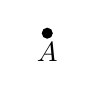
\begin{tikzpicture}
			\centering
			\fill (0,0) circle (2pt) node[below] {$A$};
		\end{tikzpicture}
	\end{center}
\end{example}
\smallskip
\textbf{خط راست:}
از مفاهیم تعریف‌نشده است. خط با دو نقطه‌ی متمایز از آن و گاهی با یک حرف کوچک نمایش داده می‌شود؛ مانند خط $AB$ یا خط $d$.
\begin{example}
	خط
	$\ell$:
	\begin{center}
		\begin{tikzpicture}
			\draw[thick] (-2,0) -- (3,0) node[below] {$\ell$};
		\end{tikzpicture}
	\end{center}
\end{example}
\smallskip
\textbf{نیم‌خط راست:}
مجموعه‌ای از نقطه‌های خط راست است که در یک طرف نقطه‌ی ثابتی از آن خط راست قرار دارد. این نقطه‌ی ثابت را مبدأ نیم‌خط می‌نامند؛ مانند نیم‌خط $Ox$.
\begin{example}
	نیم‌خط $Ox$:
	\begin{center}
		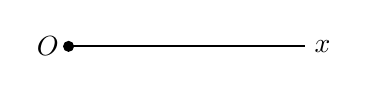
\begin{tikzpicture}
			\draw[thick] (0,0) -- (3,0);
			\fill (0,0) circle (2pt) node[left] {$O$};
			\node[right] at (3,0) {$x$};
		\end{tikzpicture}
	\end{center}
\end{example}
\smallskip
\textbf{پاره‌خط راست:}
بخشی از یک خط راست است که از دو طرف به دو نقطه محدود باشد؛ مانند پاره‌خط $AB$.
\begin{example}
	پاره‌خط $AB$:
	\begin{center}
		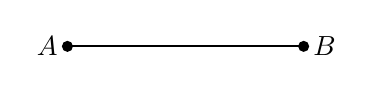
\begin{tikzpicture}
			\draw[thick] (0,0) -- (3,0);
			\fill (0,0) circle (2pt) node[left] {$A$};
			\fill (3,0) circle (2pt) node[right] {$B$};
		\end{tikzpicture}
	\end{center}
\end{example}
\begin{example}
	روی خط راستی، ۵۰ پاره‌خط راست داده شده است. ثابت کنید دست‌کم یکی از دو حکم زیر درست است:
	\begin{enumerate}
		\item 
		هشت پاره‌خط راست پیدا می‌شود که دارای نقطه‌ی مشترکی هستند.
		\item 
		هشت پاره‌خط راست وجود دارد که هیچ دوتایی از آن‌ها نقطه‌ی مشترکی ندارند.
	\end{enumerate}
	\textbf{پاسخ:}
\end{example}
\smallskip
\textbf{زاویه:}
شکلی است که از دو نیم‌خط با مبدأ مشترک پدید می‌آید. مبدأ مشترک، رأس زاویه و هر یک از دو نیم‌خط یک ضلع زاویه نامیده می‌شود؛ مانند زاویه‌ی $xOy$. گاهی زاویه را فقط با حرف رأس آن نمایش می‌دهند؛ مانند زاویه‌ی $O$. گاهی هم از یک حرف که در مجاورت رأس و بین دو ضلع نوشته می‌شود، استفاده می‌شود؛ مانند زاویه‌ی
$\alpha$.
زاویه را با نماد
$\angle$
نشان می‌دهند، مانند
$\angle xOy$.
\begin{example}
	زاویه‌ی $xOy$:
	\begin{center}
		\begin{tikzpicture}
			\coordinate (O) at (0,0);
			\coordinate (x) at (3,0);
			\coordinate (y) at (2,2.5);
			\draw[thick] (O) -- (x) node[right] {$x$};
			\draw[thick] (O) -- (y) node[right] {$y$};
			\fill (O) circle (2pt) node[below left] {$O$};
			\pic[draw, angle eccentricity=1.6, angle radius=0.8cm] {angle = x--O--y};
		\end{tikzpicture}
	\end{center}
\end{example}
\smallskip
\textbf{زاویه‌ی نیم‌صفحه:}
زاویه‌ای است که دو ضلع آن در یک امتداد باشند.
\begin{example}
	زاویه‌ی نیم‌صفحه‌ی $xOy$:
	\begin{center}
		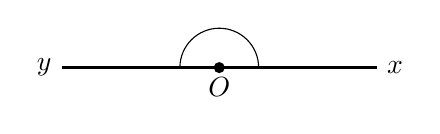
\begin{tikzpicture}
			\coordinate (O) at (0,0);
			\coordinate (x) at (2,0);
			\coordinate (y) at (-2,0);
			\draw[thick] (O) -- (x) node[right] {$x$};
			\draw[thick] (O) -- (y) node[left] {$y$};
			\fill (O) circle (2pt) node[below] {$O$};
			\pic[draw, angle eccentricity=1.6, angle radius=0.5cm] {angle = x--O--y};
		\end{tikzpicture}
	\end{center}
\end{example}
\smallskip
\textbf{نیمساز زاویه:}
نیم‌خطی است که مبدأ آن رأس زاویه است و زاویه را به دو زاویه‌ی مساوی تقسیم می‌کند.
\begin{example}
	نیم‌خط $OC$ نیمساز زاویه‌ی $AOB$ است؛ یعنی
	$\angle AOC = \angle BOC$.
	\begin{center}
		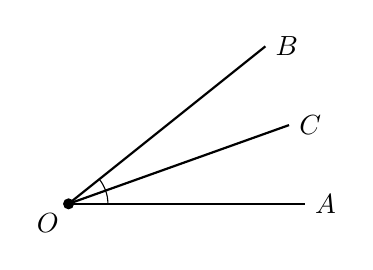
\begin{tikzpicture}
			\coordinate (O) at (0,0);
			\coordinate (A) at (3,0);
			\coordinate (B) at (2.5,2);
			\coordinate (C) at (2.8,1);
			\draw[thick] (O) -- (A) node[right] {$A$};
			\draw[thick] (O) -- (B) node[right] {$B$};
			\draw[thick] (O) -- (C) node[right] {$C$};
			\fill (O) circle (2pt) node[below left] {$O$};
			\pic[draw, angle eccentricity=1.5, angle radius=0.5cm] {angle = A--O--C};
			\pic[draw, angle eccentricity=1.5, angle radius=0.5cm] {angle = C--O--B};
		\end{tikzpicture}
	\end{center}
\end{example}
\begin{theorem}
	هر زاویه فقط یک نیمساز دارد.
	\\ \dfth \\
	\textbf{برهان:}
	اگر $Oz$ و $Ot$ هر دو نیمساز
	$\angle xOy$
	باشند، داریم:
	\[
	\begin{rcases}
		\angle xOz = \frac{1}{2} \angle xOy \\
		\angle xOt = \frac{1}{2} \angle xOy
	\end{rcases}
	\Rightarrow \angle xOz = \angle xOt
	\]
چون این دو زاویه‌ی مساوی در رأس $O$ و در ضلع $Ox$ مشترکند و در یک طرف آن ضلع قرار دارند، الزاماً دو ضلع دیگر آن‌ها بر هم منطبق می‌شوند. پس
$\angle xOy$
فقط یک نیمساز دارد.
\qed
\end{theorem}
\smallskip
\textbf{اندازه‌ی زاویه:}
نسبت آن زاویه است به زاویه‌ای که به عنوان واحد اختیار شده است.
\\
\textbf{واحد اندازه‌گیری زاویه:}
واحدی است که به‌کمک آن می‌توان اندازه‌ی زاویه‌ها را تعیین کرد. یکی از واحدهای اندازه‌گیری زاویه،
\textbf{درجه}
است که
$\frac{1}{180}$
زاویه‌ی نیم‌صفحه است. علامت درجه
$\circ$
است، مثلاً
$\ang{180}$
را ۱۸۰ درجه می‌خوانیم.
یکی دیگر از واحدهای اندازه‌گیری زاویه،
\textbf{رادیان}
است که
$\frac{1}{\pi}$
زاویه‌ی نیم‌صفحه است. اگر اندازه‌ی یک زاویه را برحسب درجه با $D$ و برحسب رادیان با $R$ نمایش دهیم، بین $D$ و $R$ رابطه‌ی
$\frac{D}{180}=\frac{R}{\pi}$
برقرار است.
\begin{example}
	زاویه‌ی
	$\frac{\pi}{3}$
	رادیان برابر با
	$\ang{60}$
	است.
\end{example}
\smallskip
\textbf{زاویه‌ی قائمه:}
نصف زاویه‌ی نیم‌صفحه است. اندازه‌ی زاویه‌ی قائمه برابر ۹۰ درجه یا
$\frac{\pi}{2}$
رادیان است. زاویه‌ی قائمه را زاویه‌ی راست نیز می‌نامند.
\begin{example}
	زاویه‌ی قائمه‌ی $xOy$:
	\begin{center}
		\begin{tikzpicture}
			\coordinate (O) at (0,0);
			\coordinate (x) at (2,0);
			\coordinate (y) at (0,2);
			\draw[thick] (O) -- (x) node[right] {$x$};
			\draw[thick] (O) -- (y) node[left] {$y$};
			\fill (O) circle (2pt) node[below] {$O$};
			\pic[draw, angle eccentricity=1.6, angle radius=0.5cm] {angle = x--O--y};
		\end{tikzpicture}
	\end{center}
\end{example}
\smallskip
\textbf{زاویه‌ی تند (حاده):}
زاویه‌ای است که از زاویه‌ی قائمه کوچک‌تر است. اندازه‌ی زاویه‌ی تند بین صفر و ۹۰ درجه است.
\begin{example}
	زاویه‌ی تند (حاده) $xOy$:
	\begin{center}
		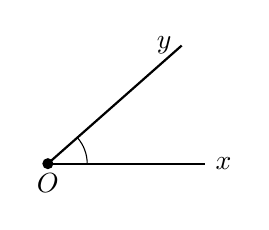
\begin{tikzpicture}
			\coordinate (O) at (0,0);
			\coordinate (x) at (2,0);
			\coordinate (y) at (1.7,1.5);
			\draw[thick] (O) -- (x) node[right] {$x$};
			\draw[thick] (O) -- (y) node[left] {$y$};
			\fill (O) circle (2pt) node[below] {$O$};
			\pic[draw, angle eccentricity=1.6, angle radius=0.5cm] {angle = x--O--y};
		\end{tikzpicture}
	\end{center}
\end{example}
\smallskip
\textbf{زاویه‌ی باز (منفرجه):}
زاویه‌ای است بزرگ‌تر از زاویه‌ی قائمه و کوچک‌تر از زاویه‌ی نیم‌صفحه. اندازه‌ی زاویه‌ی باز بین ۹۰ درجه و ۱۸۰ درجه است.
\begin{example}
	زاویه‌ی باز (منفرجه) $xOy$:
	\begin{center}
		\begin{tikzpicture}
			\coordinate (O) at (0,0);
			\coordinate (x) at (2.5,0);
			\coordinate (y) at (-2,1.5);
			\draw[thick] (O) -- (x) node[right] {$x$};
			\draw[thick] (O) -- (y) node[left] {$y$};
			\fill (O) circle (2pt) node[below] {$O$};
			\pic[draw, angle eccentricity=1.6, angle radius=0.5cm] {angle = x--O--y};
		\end{tikzpicture}
	\end{center}
\end{example}
\smallskip
\textbf{زاویه‌ی صفر:}
زاویه‌ای است که دو ضلع آن بر هم منطبق‌اند.
\begin{example}
	زاویه‌ی صفر $xOy$:
	\begin{center}
		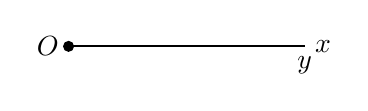
\begin{tikzpicture}
			\coordinate (O) at (0,0);
			\coordinate (x) at (3,0);
			\coordinate (y) at (3,0);
			\draw[thick] (O) -- (x) node[below] {$y$};
			\draw[thick] (O) -- (y) node[right] {$x$};
			\fill (O) circle (2pt) node[left] {$O$};
		\end{tikzpicture}
	\end{center}
\end{example}
\smallskip
\textbf{زاویه‌ی کوژ (محدب):}
زاویه‌ای است که از زاویه‌ی نیم‌صفحه کوچک‌تر است. اندازه‌ی زاویه‌ی کوژ بین صفر و ۱۸۰ درجه است.
\\
\textbf{زاویه‌ی کاو (مقعر):}
زاویه‌ای است که از زاویه‌ی نیم‌صفحه بزرگ‌تر است. اندازه‌ی زاویه‌ی کاو از ۱۸۰ درجه بیشتر است.
\begin{example}
	زاویه‌ی کاو $xOy$:
	\begin{center}
		\begin{tikzpicture}
			\coordinate (O) at (0,0);
			\coordinate (x) at (2.5,0);
			\coordinate (y) at (-2,-1.5);
			\draw[thick] (O) -- (x) node[right] {$x$};
			\draw[thick] (O) -- (y) node[left] {$y$};
			\fill (O) circle (2pt) node[below] {$O$};
			\pic[draw, angle eccentricity=1.6, angle radius=0.5cm] {angle = x--O--y};
		\end{tikzpicture}
	\end{center}
\end{example}
\smallskip
\textbf{دو زاویه‌ی مجاور:}
دو زاویه‌ای هستند که در رأس و یک ضلع مشترکند و دو ضلع غیرمشترک آن‌ها در دو طرف ضلع مشترکشان قرار دارد.
\begin{example}
	دو زاویه‌ی $AOC$ و $BOC$ مجاور (همسایه) هستند.
	\begin{center}
		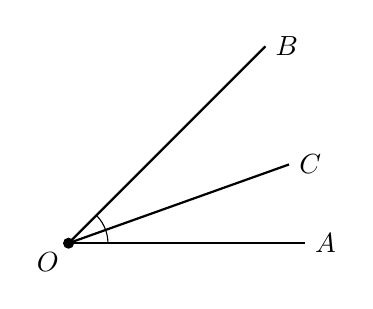
\begin{tikzpicture}
			\coordinate (O) at (0,0);
			\coordinate (A) at (3,0);
			\coordinate (B) at (2.5,2.5);
			\coordinate (C) at (2.8,1);
			\draw[thick] (O) -- (A) node[right] {$A$};
			\draw[thick] (O) -- (B) node[right] {$B$};
			\draw[thick] (O) -- (C) node[right] {$C$};
			\fill (O) circle (2pt) node[below left] {$O$};
			\pic[draw, angle eccentricity=1.5, angle radius=0.5cm] {angle = A--O--C};
			\pic[draw, angle eccentricity=1.5, angle radius=0.5cm] {angle = C--O--B};
		\end{tikzpicture}
	\end{center}
\end{example}
\smallskip
\textbf{دو زاویه‌ی متمم:}
دو زاویه‌ای هستند که مجموع آن‌ها یک زاویه‌ی قائمه است. به بیان دیگر، مجموع اندازه‌های آن‌ها برابر ۹۰ درجه است. دو زاویه‌ی متمم لزوماً مجاور نیستند.
\begin{example}
	دو زاویه‌ی
	$\ang{40}$ و $\ang{50}$
	متمم یکدیگر هستند.
\end{example}
\smallskip
\textbf{دو زاویه‌ی مکمل:}
دو زاویه‌ای هستند که مجموع آن‌ها یک زاویه‌ی نیم‌صفحه است. به بیان دیگر، مجموع اندازه‌های آن‌ها برابر ۱۸۰ درجه است. دو زاویه‌ی مکمل لزوماً مجاور نیستند.
\begin{example}
	دو زاویه‌ی
	$\ang{110}$ و $\ang{70}$
	مکمل یکدیگر هستند.
\end{example}
\smallskip
\textbf{دو زاویه‌ی مجانب:}
دو زاویه‌ای هستند که مکمل و مجاورند.
\begin{example}
	دو زاویه‌ی $AOC$ و $BOC$ مجانب هستند.
	\begin{center}
		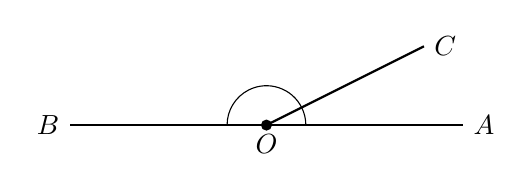
\begin{tikzpicture}
			\coordinate (O) at (0,0);
			\coordinate (A) at (2.5,0);
			\coordinate (B) at (-2.5,0);
			\coordinate (C) at (2,1);
			\draw[thick] (O) -- (A) node[right] {$A$};
			\draw[thick] (O) -- (B) node[left] {$B$};
			\draw[thick] (O) -- (C) node[right] {$C$};
			\fill (O) circle (2pt) node[below] {$O$};
			\pic[draw, angle eccentricity=1.5, angle radius=0.5cm] {angle = A--O--C};
			\pic[draw, angle eccentricity=1.5, angle radius=0.5cm] {angle = C--O--B};
		\end{tikzpicture}
	\end{center}
\end{example}
\smallskip
\textbf{دو زاویه‌ی متقابل به رأس:}
دو زاویه را که رأس مشترک داشته باشند و ضلع‌های آن‌ها دوبه‌دو در امتداد یکدیگر و در جهت‌های مخالف باشند، متقابل به رأس می‌گوییم.
\begin{example} \label{geexmotaberas}
	دو زاویه‌ی $xOy$ و $x'Oy'$ متقابل به رأس هستند.
	\begin{center}
		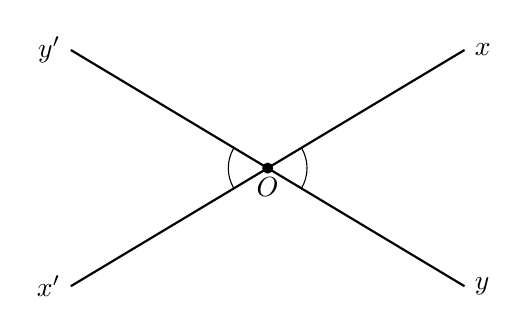
\begin{tikzpicture}
			\coordinate (O) at (0,0);
			\coordinate (x1) at (2.5,1.5);
			\coordinate (y1) at (2.5,-1.5);
			\coordinate (x2) at (-2.5,-1.5);
			\coordinate (y2) at (-2.5,1.5);
			\draw[thick] (O) -- (x1) node[right] {$x$};
			\draw[thick] (O) -- (y1) node[right] {$y$};
			\draw[thick] (O) -- (x2) node[left] {$x'$};
			\draw[thick] (O) -- (y2) node[left] {$y'$};
			\fill (O) circle (2pt) node[below] {$O$};
			\pic[draw, angle eccentricity=1.5, angle radius=0.5cm] {angle = y1--O--x1};
			\pic[draw, angle eccentricity=1.5, angle radius=0.5cm] {angle = y2--O--x2};
		\end{tikzpicture}
	\end{center}
\end{example}
\begin{theorem}
	دو زاویه‌ی متقابل به رأس مساوی هستند.
	\\ \dfth \\
	\textbf{برهان:}
	دو زاویه‌ی متقابل به رأس $xOy$ و $x'Oy'$ مثال
	\ref{geexmotaberas}
	را در نظر بگیرید. با فرض
	$\angle xOy = \alpha$ و $\angle x'Oy' = \beta$ و $\angle xOy' = \gamma$
	داریم:
	\[
	\begin{cases}
		\angle yOy' = \ang{180} \Rightarrow \alpha + \gamma = \ang{180} \\
		\angle xOx' = \ang{180} \Rightarrow \beta + \gamma = \ang{180}
	\end{cases}
	\Rightarrow \ \alpha = \beta \ \Rightarrow \ \angle xOy = \angle x'Oy'
	\]
	\qed
\end{theorem}
\begin{theorem}
	اگر دو زاویه‌ی مساوی رأس مشترک داشته باشند و یک ضلع از یکی با یک ضلع از دیگری بر امتداد یک خط راست و در دو جهت مخالف باشد و دو ضلع دیگر آن‌ها متمایز با آن خط راست و در دو طرف آن خط راست باشند، دو زاویه‌ی متقابل به رأس تشکیل می‌دهند (یعنی دو ضلع دیگر آن‌ها نیز بر امتداد یک خط راست هستند).
	\\ \dfth \\
	\textbf{برهان:}
	شکل مثال
	\ref{geexmotaberas}
	را در نظر بگیرید. اگر
	$\angle xOy = \angle x'Oy'$
	و $xOx'$ خط راست باشد، می‌خواهیم ثابت کنیم که
	$yOy'$
	نیز خط راست است.  با فرض
	$\angle xOy = \alpha$ و $\angle x'Oy' = \beta$ و $\angle xOy' = \gamma$
	داریم:
	\[
	\begin{rcases}
		\angle xOx' = \ang{180} \Rightarrow \beta + \gamma = \ang{180} \\
		\angle xOy = \angle x'Oy' \ \Rightarrow \ \alpha = \beta
	\end{rcases}
	\Rightarrow \alpha + \gamma = \ang{180} \ \Rightarrow \ \angle xOy + \angle xOy' = \angle yOy' = \ang{180}
	\]
	\qed
\end{theorem}
\begin{theorem}
	نیمسازهای دو زاویه‌ی متقابل به رأس بر یک خط راست واقع هستند.
	\\ \dfth \\
	\textbf{برهان:}
	
\end{theorem}
%%%%%%%%%%%%%%%%%%%%%%%%%%%%%%%%%%%%%%%%%%%%%
\bigskip
\textbf{اصول پنجگانه‌ی اقلیدس:}
\begin{enumerate}
	\item 
	به‌ازای هر نقطه‌ی $P$ و هر نقطه‌ی $Q$ که با $P$ مساوی نباشد، خط یکتایی مانند $L$ وجود دارد که بر $P$ و $Q$ می‌گذرد. (هر دو نقطه‌ی متمایز یک خط راست منحصربه‌فرد را مشخص می‌سازند.)
	\item 
	به‌ازای هر پاره‌خط $AB$ و هر پاره‌خط $CD$، نقطه‌ی منحصربه‌فردی چون $E$ وجود دارد، چنان‌که $B$ میان $A$ و $E$ واقع است و پاره‌خط $CD$ با پاره‌خط $BE$ قابل انطباق است. (هر پاره‌خط $AB$ را می‌توان به اندازه‌ی پاره‌خط $BE$ که با پاره‌خط داده‌شده‌ی $CD$ قابل انطباق است، امتداد داد.)
	\item 
	به‌ازای هر نقطه‌ی $O$ و هر نقطه‌ی $A$ که با $O$ مساوی نباشد، دایره‌ای به مرکز $O$ و به شعاع $OA$ وجود دارد.
	\item 
	همه‌ی زاویه‌های قائمه
	($\ang{90}$)
	با یکدیگر قابل انطباق‌اند (برابرند).
	\item 
	اگر دو خط به‌وسیله‌ی خط موربی چنان قطع شوند که مجموع اندازه‌های دو زاویه‌ی درونی واقع در یک طرف خط مورب کمتر از
	$\ang{180}$
	باشد، اگر این دو خط را بی‌نهایت امتداد دهیم، آنگاه این دو خط همدیگر را در همان طرف خط مورب، قطع می‌کنند.
\end{enumerate}
\smallskip
\textbf{اصل توازی پلی‌فیر:}
به‌ازای هر خط $L$ و هر نقطه‌ی $P$ غیر واقع بر آن، تنها یک خط مانند $m$ وجود دارد چنان‌که از $P$ می‌گذرد و با $L$ موازی است.

\section{مثلث}

\section{چندضلعی‌ها}

\section{دایره}

	\chapter{هندسه‌ی تحلیلی}
\thispagestyle{empty}

\begin{quote}
	{\lotus
		هندسه‌ی تحلیلی هرگز وجود نداشته است. فقط افرادی وجود دارند که با استفاده از مختصات، هندسه‌ی خطی را بد انجام می‌دهند و آن را هندسه‌ی تحلیلی می‌نامند. آن‌ها را بیرون کنید! \quad - دیودنه%
		\LTRfootnote{ Jean Alexandre Eug\`{e}ne Dieudonn\'{e}}
	}
\end{quote}

	\chapter{هندسه‌ی فضایی}
\thispagestyle{empty}

\begin{quote}
	{\lotus
		اولین آزمون برای این که ببینید استعدادی در ریاضیات دارید این است که ببینید آیا می‌توانید چیزی از هندسه دریابید. \quad - لیتلوود%
		\LTRfootnote{ John Edensor Littlewood}
	}
\end{quote}

	
	\part{جبر خطی}
	\chapter{ماتریس و دترمینان}
\thispagestyle{empty}

\begin{quote}
	{\lotus
		ما [او و هالموس] فلسفه‌ی مشترکی درمورد جبر خطی داریم؛ فارغ از پایه فکر می‌کنیم، فارغ از پایه می‌نویسیم، اما هنگامی که کار به جای باریک می‌رسد درِ اتاق کارمان را می‌بندیم و با عصبانیت آن را با ماتریس‌ها محاسبه می‌کنیم. \quad - کاپلانسکی%
		\LTRfootnote{ Irving Kaplansky}
	}
\end{quote}

\section{ماتریس}
 هر آرایش مستطیلی از اعداد، شامل تعدادی سطر و ستون یک ماتریس نامیده می‌شود. هر عدد واقع در هر ماتریس را درایه‌ی آن ماتریس می‌نامیم. معمولاً ماتریس‌ها را با حروف بزرگ مانند $A$، $B$، $C$ و ... نام‌گذاری می‌کنیم.

در حالت کلی، اگر ماتریسی چون $A$ دارای $m$ سطر و $n$ ستون باشد، می‌نویسیم
$A_{m \times n}$
و می‌خوانیم $A$ ماتریسی از مرتبه‌ی $m$ در $n$ است. برای هر درایه‌ی ماتریس دو اندیس در نظر می‌گیریم که اندیس سمت چپ جای سطر و اندیس سمت راست جای ستون آن درایه را مشخص می‌کند،
$a_{ij}$
یعنی درایه‌ی روی سطر $i$ و ستون $j$.
\[
A = \begin{bmatrix}
	a_{11} & a_{12} & \cdots & a_{1n} \\
	a_{21} & a_{22} & \cdots & a_{2n} \\
	\vdots & \vdots & \ddots & \vdots \\
	a_{m1} & a_{m2} & \cdots & a_{mn}
\end{bmatrix}
\]

\begin{example}
	ماتریس $B$ ماتریسی شامل دو سطر و سه ستون است. این ماتریس دارای
	$2 \times 3 = 6$
	درایه است و مثلاً عدد
	$\sqrt{3}$
	درایه‌ی روی سطر اول و ستون اول است و درایه‌ی
	$(-4)$
	روی سطر دوم و ستون سوم قرار دارد.
	\[
	B = \begin{bmatrix}
		\sqrt{3} & 0 & \dfrac{2}{5} \\
		\pi & 6 & -4
	\end{bmatrix}
	\]
\end{example}

\begin{example}
	ماتریس
	$A=[a_{ij}]_{2 \times 2}$
	را در نظر بگیرید. اگر برای
	$i=j$
	داشته باشیم
	$a_{ij}=9$
	و برای
	$i>j$
	داشته باشیم
	$a_{ij}=-4$
	 و برای
	 $i<j$
	 داشته باشیم
	 $a_{ij}=6$،
	 در این صورت ماتریس $A$ را با درایه‌هایش نمایش دهید.
	 \\
	 پاسخ:
	 \[
	 A = \begin{bmatrix}
	 	9 & 6 \\
	 	-4 & 9
	 \end{bmatrix}
	 \]
\end{example}
\bigskip
دو ماتریس هم‌مرتبه‌ی
$A=[a_{ij}]_{m \times n}$
و
$B=[b_{ij}]_{m \times n}$
را مساوی گوییم هرگاه درایه‌های نظیر به نظیر آن‌ها با هم برابر باشند.
$$\forall i,j : a_{ij} = b_{ij} \Leftrightarrow [a_{ij}] = [b_{ij}]$$

\begin{example}
	اگر دو ماتریس
	$A = \begin{bmatrix}
		x-y & 8 \\
		4 & z-1
	\end{bmatrix}$
	و
	$B = \begin{bmatrix}
		2 & x+y \\
		4 & 6
	\end{bmatrix}$
	مساوی باشند،
	$(x+y+z)$
	را بیابید. \\
	\textbf{پاسخ:}
	\[
	A=B \Rightarrow
	\begin{cases}
		x-y=2 \\
		x+y=8 \\
		z-1=6
	\end{cases}
	\Rightarrow
	x=5 , y=3 , z=7
	\Rightarrow
	x+y+z=15
	\]
\end{example}

\subsection{ماتریس‌های خاص}
\textbf{ماتریس مربعی:}
اگر در ماتریس $A$، تعداد سطرها با تعداد ستون‌ها برابر و مساوی $n$ باشد، $A$ را یک ماتریس مربعی از مرتبه‌ی $n$ می‌نامیم. اگر
$i=j$
در این صورت درایه‌ی
$a_{ij}$
روی
\textbf{قطر اصلی}
ماتریس قرار دارد.
\begin{example}
	\[
	A = \begin{bmatrix}
		5 \\
	\end{bmatrix}_{1 \times 1}
	= 5
	\qquad
	B = \begin{bmatrix}
		1 & 2 \\
		-1 & 0
	\end{bmatrix}_{2 \times 2}
	\qquad
	C = \begin{bmatrix}
		2 & 1 & 3 \\
		-4 & 5 & 0 \\
		3 & 7 & 8
	\end{bmatrix}_{3 \times 3}
	\]
\end{example}
\smallskip
\textbf{ماتریس سطری:}
اگر ماتریس $A$ فقط دارای یک سطر باشد، آن را یک ماتریس سطری می‌نامیم.
\begin{example}
	\[
	A = \begin{bmatrix}
		11
	\end{bmatrix}_{1 \times 1}
	=11
	\qquad
	B = \begin{bmatrix}
		3 & 7
	\end{bmatrix}_{1 \times 2}
	\qquad
	C = \begin{bmatrix}
		2 & -1 & 4 & 6
	\end{bmatrix}_{1 \times 4}
	\]
\end{example}
\smallskip
\textbf{ماتریس ستونی:}
اگر ماتریس $A$ فقط دارای یک ستون باشد، آن را یک ماتریس ستونی می‌نامیم.
\begin{example}
	\[
	A = \begin{bmatrix}
		23
	\end{bmatrix}_{1 \times 1}
	=23
	\qquad
	B = \begin{bmatrix}
		0 \\
		\sqrt{60} \\
		-53 \\
		\pi
	\end{bmatrix}_{4 \times 1}
	\]
\end{example}
\smallskip
\textbf{ماتریس قطری:}
ماتریس قطری، ماتریسی است مربعی که تمام درایه‌های غیرواقع بر قطر اصلی آن صفر باشند. درایه‌های واقع بر قطر اصلی می‌توانند صفر باشند یا نباشند.
\begin{example}
	\[
	A = \begin{bmatrix}
		2 & 0 \\
		0 & 7
	\end{bmatrix}
	\qquad
	B = \begin{bmatrix}
		-1 & 0 & 0 \\
		0 & 0 & 0 \\
		0 & 0 & 8
	\end{bmatrix}
	\qquad
	C = \begin{bmatrix}
		0 & 0 & 0 \\
		0 & 0 & 0 \\
		0 & 0 & 0
	\end{bmatrix}
	\]
\end{example}
\smallskip
\textbf{ماتریس اسکالر:}
اگر ماتریسی قطری باشد و تمام درایه‌های روی قطر اصلی آن با هم برابر باشند، آن را یک ماتریس اسکالر می‌نامیم.
\begin{example} \label{exmatsca}
	\[
	A = \begin{bmatrix}
		3
	\end{bmatrix}
	\qquad
	B = \begin{bmatrix}
		1 & 0 \\
		0 & 1
	\end{bmatrix}
	\qquad
	C = \begin{bmatrix}
		5 & 0 & 0 \\
		0 & 5 & 0 \\
		0 & 0 & 5
	\end{bmatrix}
	\]
\end{example}
\smallskip
\textbf{ماتریس واحد یا همانی:}
ماتریس اسکالری که درایه‌های قطر اصلی آن یک باشد، ماتریس واحد یا همانی نامیده می‌شود. ماتریس همانی مرتبه‌ی $n$ را با نماد
$I_n$
نشان می‌دهند. در مثال
\ref{exmatsca}،
ماتریس $B$ یک ماتریس واحد یا همانی از مرتبه‌ی ۲ می‌باشد.
\\
\textbf{ماتریس صفر:}
ماتریس صفر، ماتریسی است که همه‌ی درایه‌های آن صفر باشند. ماتریس صفر را با نماد
$O$
یا
$\overline{O}$
نشان می‌دهیم.
\begin{example}
	$$O_{1 \times 2} =
	\begin{bmatrix}
		0 & 0
	\end{bmatrix}$$
\end{example}
\smallskip
\textbf{ماتریس پایین‌مثلثی:}
اگر درایه‌های بالای قطر اصلی ماتریس $A$ برابر صفر باشند، $A$ را ماتریس پایین‌مثلثی می‌نامیم. اگر درایه‌های قطر اصلی نیز برابر صفر باشند، آن ماتریس را پایین‌مثلثی اکید می‌نامیم.
\begin{example}
	ماتریس
	$
	A = \begin{bmatrix}
		1 & 0 & 0 \\
		4 & 2 & 0 \\
		5 & 3 & 7
	\end{bmatrix}
	$
	یک ماتریس پایین‌مثلثی از مرتبه‌ی ۳ است.
\end{example}
\smallskip
\textbf{ماتریس بالامثلثی:}
اگر درایه‌های پایین قطر اصلی ماتریس $A$ برابر صفر باشند، $A$ را ماتریس بالامثلثی می‌نامیم. اگر درایه‌های قطر اصلی نیز برابر صفر باشند، آن ماتریس را بالامثلثی اکید می‌نامیم.
\begin{example}
	ماتریس
	$
	B = \begin{bmatrix}
		1 & 9 & 2 \\
		0 & 3 & 5 \\
		0 & 0 & 6
	\end{bmatrix}
	$
	یک ماتریس بالامثلثی از مرتبه‌ی ۳ است.
\end{example}
\smallskip
\textbf{ترانهاده‌ی یک ماتریس:}
فرض کنیم
$A=[a_{ij}]_{m \times n}$
یک ماتریس باشد. ترانهاده‌ی $A$ که آن را با $A^t$ یا $A'$ نمایش می‌دهیم، برابر است با
$A^t=[b_{ij}]_{n \times m}$
و به صورت زیر تعریف می‌شود:
$$b_{ij} = a_{ji}$$

\begin{example}
	اگر
	$
	A = \begin{bmatrix}
		2 & \sqrt{2} \\
		-1 & 3 \\
		0 & 1
	\end{bmatrix}
	$،
	آنگاه
	$
	A^t = \begin{bmatrix}
		2 & -1 & 0 \\
		\sqrt{2} & 3 & 1
	\end{bmatrix}
	$.
\end{example}
\smallskip
\textbf{ماتریس متقارن:}
فرض کنیم
$A=[a_{ij}]_{n \times n}$
یک ماتریس باشد. $A$ را متقارن گوییم هرگاه
$A^t=A$.

\begin{example}
	مقادیر $x$ و $y$ و $z$ را چنان تعیین کنید که ماتریس $A$ متقارن باشد.
	\[
	A = \begin{bmatrix}
		1 & 3 & -2 \\
		2x-1 & 3 & y-1 \\
		3y+1 & -x & -4
	\end{bmatrix}
	\]
	\textbf{پاسخ:}
	\[
	\begin{cases}
	2x-1 = 3 \\
	3y+1 = -2 \\
	y-1 = -x
	\end{cases}
	\Rightarrow
	x=2 ,\: y=-1
	\]
	
\end{example}
\smallskip
\textbf{ماتریس پادمتقارن:}
فرض کنیم
$A=[a_{ij}]_{n \times n}$
یک ماتریس باشد. $A$ را پادمتقارن گوییم هرگاه
$A^t=-A$.

\begin{example}
	$A$
	یک ماتریس پادمتقارن مرتبه‌ی $n$ است. حاصل‌جمع همه‌ی درایه‌های $A$ چند است؟ \\
	\textbf{پاسخ:}
	درایه‌‌های واقع بر قطر اصلی همگی صفر هستند و درایه‌های غیر قطر اصلی نیز دوبه‌دو قرینه‌اند، پس مجموع همه‌ی درایه‌ها صفر است.
\end{example}

\subsection{جمع و ضرب در ماتریس‌ها}
\subsubsection*{جمع ماتریس‌ها}
برای جمع یا تفاضل دو ماتریس هم‌مرتبه‌ی $A$ و $B$ کافی است درایه‌های نظیر به نظیر دو ماتریس را با هم جمع یا از هم کم کرد.
$$A=[a_{ij}]_{m \times n} ,\ B=[b_{ij}]_{m \times n} \Rightarrow A \pm B = [a_{ij}] \pm [b_{ij}] = [a_{ij} \pm b_{ij}]$$

\begin{example}
	دو ماتریس
	$
	A = \begin{bmatrix}
		7 & 3 & 5 \\
		-5 & 2 & 0
	\end{bmatrix}
	$
	و
	$
	B = \begin{bmatrix}
		3 & 0 \\
		1 & 6 \\
		4 & 3
	\end{bmatrix}
	$
	را نمی‌توان با هم جمع کرد، چون هم‌مرتبه نیستند. ولیکن مجموع دو ماتریس
	$
	C = \begin{bmatrix}
		3 & 1 & 5 \\
		0 & 6 & 8
	\end{bmatrix}
	$
	و
	$
	D = \begin{bmatrix}
		4 & 5 & 6 \\
		9 & 2 & 1
	\end{bmatrix}
	$
	برابر است با ماتریس
	$
	C+D = \begin{bmatrix}
		7 & 6 & 11 \\
		9 & 8 & 9
	\end{bmatrix}
	$.
\end{example}

\begin{example}
	اگر
	$A=\begin{bmatrix}
		1 & 2 \\
		-3 & 5
	\end{bmatrix}$
	و
	$B=\begin{bmatrix}
		2 & -1 \\
		3 & 4
	\end{bmatrix}$،
	آنگاه
	$(A+B)^t$
	و
	$A^t + B^t$
	را به دست آورید. \\
	\textbf{پاسخ:}
	\[
	A+B =
	\begin{bmatrix}
		1 & 2 \\
		-3 & 5
	\end{bmatrix}
	+
	\begin{bmatrix}
		2 & -1 \\
		3 & 4
	\end{bmatrix}
	=
	\begin{bmatrix}
		3 & 1 \\
		0 & 9
	\end{bmatrix}
	\]
	
	\[
	(A+B)^t =
	\begin{bmatrix}
		3 & 0 \\
		1 & 9
	\end{bmatrix}
	\]
	
	\[
	A^t + B^t =
	\begin{bmatrix}
		1 & -3 \\
		2 & 5
	\end{bmatrix}
	+
	\begin{bmatrix}
		2 & 3 \\
		-1 & 4
	\end{bmatrix}
	=
	\begin{bmatrix}
		3 & 0 \\
		1 & 9
	\end{bmatrix}
	\]
\end{example}

\subsubsection*{ضرب یک عدد در یک ماتریس}
برای ضرب یک عدد در ماتریسی چون $A$ آن عدد را در تمام درایه‌های ماتریس ضرب می‌کنیم.
$$A=[a_{ij}]_{m \times n} ,\ r \in \mathbb{R} \Rightarrow rA = r[a_{ij}]_{m \times n} = [ra_{ij}]_{m \times n}$$

\begin{example}
	\[
	-2 \times
	\begin{bmatrix}
	2 & 6 & -4 \\
	3 & -2 & 0
	\end{bmatrix}
	=
	\begin{bmatrix}
		-4 & -12 & 8 \\
		-6 & 4 & 0
	\end{bmatrix}
	\]
\end{example}
\bigskip
\textbf{قرینه‌ی ماتریس:}
اگر
$A=[a_{ij}]_{m \times n}$
ماتریسی دلخواه باشد، قرینه‌ی ماتریس $A$ را با
$(-A)$
نمایش داده و از ضرب
$(-1)$
در ماتریس $A$ به دست می‌آید.

\subsubsection*{خواص مهم جمع ماتریس‌ها و ضرب عدد در ماتریس}
اگر $A$، $B$ و $C$ ماتریس‌هایی هم‌مرتبه و $r$ و $s$ اعدادی حقیقی باشند خواص زیر قابل اثبات‌اند:
\LR{
\begin{enumerate}
	\item $A+B = B+A$
	\item $A+(B+C) = (A+B)+C$
	\item $A+O = O+A = A$
	\item $A+(-A) = (-A)+A = O$
	\item $r(A \pm B) = rA \pm rB$
	\item $(r \pm s)A = rA \pm sA$
	\item $rA=rB ,\ r \neq 0 \Rightarrow A=B$
	\item $A=B \Rightarrow rA=rB$
\end{enumerate}}
\vspace*{-1cm}

\subsubsection*{ضرب ماتریس در ماتریس}
فرض کنیم
$A=[a_{ij}]_{m \times n}$
و
$B=[b_{ij}]_{n \times p}$.
حاصل‌ضرب $A$ در $B$ یعنی
$AB=[c_{ij}]_{m \times p}$
و به صورت زیر تعریف می‌شود:
$$c_{ij} = \sum_{k=1}^{n}a_{ik}b_{kj}$$
توجه کنید که تعداد ستون‌های $A$ برابر تعداد سطرهای $B$ است.

\begin{example}
	اگر
	$A=
	\begin{bmatrix}
		1 & 2 \\
		3 & 4 \\	
	\end{bmatrix}
	$
	و
	$B=
	\begin{bmatrix}
		5 & 6 \\
		7 & 8 \\	
	\end{bmatrix}
	$،
	حاصل $AB$ و $BA$ را حساب کنید. \\
	\textbf{پاسخ:}
	\[
	AB=
	\begin{bmatrix}
		1 & 2 \\
		3 & 4 \\	
	\end{bmatrix}
	\begin{bmatrix}
		5 & 6 \\
		7 & 8 \\	
	\end{bmatrix}
	=
	\begin{bmatrix}
		(1 \times 5)+(2 \times 7) & (1 \times 6)+(2 \times 8) \\
		(3 \times 5)+(4 \times 7) & (3 \times 6)+(4 \times 8) \\	
	\end{bmatrix}
	=
	\begin{bmatrix}
		19 & 22 \\
		43 & 50 \\	
	\end{bmatrix}
	\]
	\[
	BA=
	\begin{bmatrix}
		5 & 6 \\
		7 & 8 \\	
	\end{bmatrix}
	\begin{bmatrix}
		1 & 2 \\
		3 & 4 \\	
	\end{bmatrix}
	=
	\begin{bmatrix}
		(5 \times 1)+(6 \times 3) & (5 \times 2)+(6 \times 4) \\
		(7 \times 1)+(8 \times 3) & (7 \times 2)+(8 \times 4) \\	
	\end{bmatrix}
	=
	\begin{bmatrix}
		23 & 34 \\
		31 & 46 \\	
	\end{bmatrix}
	\]
\end{example}

\begin{example}
	مثال نقضی برای این گزاره بیابید: اگر حاصل‌ضرب دو ماتریس برابر صفر شود، حداقل یکی از آن‌ها صفر است. \\
	\textbf{پاسخ:}
	\[
	A=
	\begin{bmatrix}
		2 & -1 \\
		4 & -2
	\end{bmatrix},
	\qquad
	B=
	\begin{bmatrix}
		1 & 5 \\
		2 & 10
	\end{bmatrix}
	\]
	\[
	AB=
	\begin{bmatrix}
		2-2 & 10-10 \\
		4-4 & 20-20
	\end{bmatrix}
	=
	\begin{bmatrix}
		0 & 0 \\
		0 & 0
	\end{bmatrix}
	= O_2
	\]
\end{example}

\begin{example}
	با یک مثال نقض نشان دهید که در حالت کلی از تساوی
	$AB=AC$
	نمی‌توان نتیجه گرفت
	$B=C$.
	\\ \textbf{پاسخ:}
\end{example}

\begin{example}
	اگر
	$A=
	\begin{bmatrix}
		1 & -1 \\
		0 & 2
	\end{bmatrix}$،
	تمام ماتریس‌های
	$2 \times 2$
	مانند $B$ را بیابید که داشته باشیم
	$AB=BA$. \\
	\textbf{پاسخ:}
	فرض کنیم
	$B=
	\begin{bmatrix}
		a & b \\
		c & d
	\end{bmatrix}$.
	\[
	AB =
	\begin{bmatrix}
		1 & -1 \\
		0 & 2
	\end{bmatrix}
	\begin{bmatrix}
		a & b \\
		c & d
	\end{bmatrix}
	=
	\begin{bmatrix}
		a-c & b-d \\
		2c & 2d
	\end{bmatrix}
	\]
	\[
	BA =
	\begin{bmatrix}
		a & b \\
		c & d
	\end{bmatrix}
	\begin{bmatrix}
		1 & -1 \\
		0 & 2
	\end{bmatrix}
	=
	\begin{bmatrix}
		a & -a+2b \\
		c & -c+2d
	\end{bmatrix}
	\]
	\[
	AB=BA \Rightarrow
	\begin{cases}
		a-c=a \\
		2c=c \\
		b-d=-a+2b \\
		2d=-c+2d
	\end{cases}
	\Rightarrow
	c=0 , \ b=a-d
	\]
	بنابراین $a$ و $d$ اعدادی دلخواه هستند و تمام ماتریس‌های به شکل زیر پاسخ مسئله هستند.
	\[
	B=
	\begin{bmatrix}
		a & a-d \\
		0 & d
	\end{bmatrix}
	\]
\end{example}

\subsubsection*{خواص مهم ضرب ماتریس‌ها}
فرض کنیم
$A=[a_{ij}]_{m \times n}$،
$B=[b_{ij}]_{n \times p}$،
$C=[c_{ij}]_{p \times q}$ و
$D=[d_{ij}]_{n \times n}$.
در این صورت:
\LR{
	\begin{enumerate}
		\item $A(BC)=(AB)C$
		\item $A(B+C)=AB+BC$
		\item $(A+B)C=AC+BC$
		\item $DI_n=I_nD=D$
		\item $DO_n=O_nD=O_n$
\end{enumerate}}

فرض کنیم
$A=[a_{ij}]_{n \times n}$
و
$B=[b_{ij}]_{n \times n}$
دو ماتریس باشند و $r$ یک عدد حقیقی. در این صورت:
\LR{\begin{enumerate}
		\item $(A+B)^t = A^t + B^t$
		\item $(rA)^t = rA^t$
		\item $(AB)^t = B^t A^t$
		\item $(A^t)^t = A$
\end{enumerate}}

فرض کنیم
$A=[a_{ij}]_{n \times n}$.
در این صورت:
\[
\left[ \frac{1}{2}(A+A^t) \right]^t = \frac{1}{2}(A+A^t)^t = \frac{1}{2}(A^t+(A^t)^t) = \frac{1}{2}(A^t+A) = \frac{1}{2}(A+A^t)
\]
\[
\left[ \frac{1}{2}(A-A^t) \right]^t = \frac{1}{2}(A-A^t)^t = \frac{1}{2}(A^t-(A^t)^t) = \frac{1}{2}(A^t-A) = -\frac{1}{2}(A-A^t)
\]
در نتیجه
$\frac{1}{2}(A+A^t)$
ماتریس متقارن و
$\frac{1}{2}(A-A^t)$
ماتریس پادمتقارن است. اکنون با توجه به
$$A=\frac{1}{2}(A+A^t)+\frac{1}{2}(A-A^t)$$
نتیجه می‌گیریم که هر ماتریس مربعی را می‌توان به صورت مجموع یک ماترس متقارن و یک ماتریس پادمتقارن نوشت.

\textbf{تعویض‌پذیری:}
اگر $AB$ و $BA$ با هم برابر باشند، می‌گوییم ماتریس‌های $A$ و $B$ تعویض‌پذیر هستند. اگر $A$ و $B$ دو ماتریس مربعی هم‌مرتبه و تعویض‌پذیر باشند، آنگاه تمام اتحادهای جبری را درمورد آن دو ماتریس می‌توان به کار برد. همچنین اگر $m$ و $n$ دو عدد طبیعی باشند، آنگاه
$A^mB^n = B^nA^m$،
یعنی هر توانی از $A$ با هر توانی از $B$ تعویض‌پذیر است. اگر دو ماتریس تعویض‌پذیر نباشند، در نوشتن عبارت‌های جبری باید ترتیب ضرب حفظ شود. همچنین برای
$a,b,n,m \in \mathbb{N}$
داریم:
$$(A^a)^n \times (A^b)^m = (A^b)^m \times (A^a)^n= A^{an+bm}$$

\begin{example}
	اگر
	$A^3=
	\begin{bmatrix}
		3 & 2 \\
		2 & 1
	\end{bmatrix}$ و
	$A^4=
	\begin{bmatrix}
		5 & 3 \\
		3 & 2
	\end{bmatrix}$
	باشد، ماتریس
	$A^{11}$
	را به دست آورید. \\
	\textbf{پاسخ:}
	باید بررسی کنیم که ۱۱ را چگونه می‌توان به‌صورت جمع ضریبی از ۴ و ضریبی از ۳ نوشت:
	$$11=2 \times 4 + 3 \times 1 \Rightarrow A^{11} = (A^4)^2 \times (A^3)^1$$
	\[
	(A^4)^2=
	\begin{bmatrix}
		5 & 3 \\
		3 & 2
	\end{bmatrix}
	\begin{bmatrix}
		5 & 3 \\
		3 & 2
	\end{bmatrix}
	=
	\begin{bmatrix}
		34 & 21 \\
		21 & 13
	\end{bmatrix}
	\]
	\[
	A^{11}=(A^4)^2 \times A^3=
	\begin{bmatrix}
		34 & 21 \\
		21 & 13
	\end{bmatrix}
	\begin{bmatrix}
		3 & 2 \\
		2 & 1
	\end{bmatrix}
	=
	\begin{bmatrix}
		144 & 89 \\
		89 & 55
	\end{bmatrix}
	\]
\end{example}
\smallskip
\textbf{ماتریس خودتوان:}
ماتریس مربعی $A$ را خودتوان گویند هرگاه
$A^2=A$.
اگر یک ماتریس خودتوان باشد، آنگاه به ازای هر عدد طبیعی $n$ داریم
$A^n=A$.

\begin{example}
	تمام ماتریس‌هایی به صورت
	$A=
	\begin{bmatrix}
		a & 1 \\
		0 & b
	\end{bmatrix}$
	را بیابید که خودتوان باشند. \\
	\textbf{پاسخ:}
	\[
	A^2=
	\begin{bmatrix}
		a & 1 \\
		0 & b
	\end{bmatrix}
	\begin{bmatrix}
		a & 1 \\
		0 & b
	\end{bmatrix}
	=
	\begin{bmatrix}
		a^2 & a+b \\
		0 & b^2
	\end{bmatrix}
	\]
	\[
	A^2=A \Rightarrow
	\begin{bmatrix}
		a^2 & a+b \\
		0 & b^2
	\end{bmatrix}
	=
	\begin{bmatrix}
		a & 1 \\
		0 & b
	\end{bmatrix}
	\Rightarrow
	\begin{cases}
		a^2=a \\
		a+b=1 \\
		b^2=b
	\end{cases}
	\Rightarrow
	\begin{cases}
		a=0 \\
		b=1
	\end{cases}
	\text{یا} \
	\begin{cases}
		a=1 \\
		b=0
	\end{cases}
	\]
	بنابراین:
	\[
	A=
	\begin{bmatrix}
		0 & 1 \\
		0 & 1
	\end{bmatrix}
	\quad \text{یا} \quad
	A=
	\begin{bmatrix}
		1 & 1 \\
		0 & 0
	\end{bmatrix}
	\]
\end{example}

\begin{example}
	اگر $A$ خودتوان و $I$ ماتریس همانی هم‌مرتبه با $A$ باشد، حاصل
	$(A+I)^3$
	چیست؟ \\
	\textbf{پاسخ:}
	$A$ و $I$
	تعویض‌پذیرند. بنابراین:
	$$(A+I)^3 = A^3 + 3A^2 + 3A + I = A + 3A + 3A + I = 7A + I$$
\end{example}

\begin{theorem}
	اگر $A$ خودتوان و $I$ ماتریس همانی هم‌مرتبه با $A$ باشد، به ازای هر عدد طبیعی $n$ داریم:
	$$(A+I)^n = (2^n-1)A + I$$
\end{theorem}

\section{دترمینان}
به هر ماتریس مربعی می‌توان یک عدد نسبت داد که دترمینان آن ماتریس نامیده می‌شود. دترمینان یک ماتریس اطلاعات مفیدی راجع‌به خود ماتریس و خواص آن به ما خواهد داد.

اگر $A$ ماتریسی مربعی از مرتبه‌ی $n$ باشد، در این صورت دترمینان ماتریس $A$ را با نماد
$\det(A)=|A|$
نمایش می‌دهیم. برای ماتریس‌های مربعی مرتبه‌ی ۱ و ۲ داریم:
\[
A=[k]_{1 \times 1} \Rightarrow |A|=k
\]
\[
B=
\begin{bmatrix}
	a & b \\
	c & d \\	
\end{bmatrix}
\Rightarrow
|B|=ad-bc
\]

\begin{example}
	دترمینان ماتریس
	$A=\begin{bmatrix}
		\sin\alpha & \cos\alpha \\
		-\cos\alpha & \sin\alpha \\	
	\end{bmatrix}$
	را به دست آوردید.
	\[
	|A|=\sin^2\alpha + \cos^2\alpha = 1
	\]
\end{example}

پیش از تعریف دترمینان برای ماتریس مربعی مرتبه‌ی ۳ و بالاتر لازم است با چند تعریف دیگر آشنا شویم.
\\
\textbf{کهاد:}
فرض کنیم
$A=[a_{ij}]_{n \times n}$
ماتریسی دلخواه باشد. در این صورت $ij$-امین کهاد ماتریس $A$ را که با
$M_{ij}$
نمایش می‌دهیم، ماتریسی
$(n-1) \times (n-1)$
تعریف می‌کنیم که از حذف سطر $i$ و ستون $j$ ماتریس $A$ به دست می‌آید.

\begin{example}
	برای ماتریس
	$A=
	\begin{bmatrix}
		2 & -1 & 4 \\
		0 & 1 & 5 \\
		6 & 3 & -4
	\end{bmatrix}$،
	داریم
	$M_{13}=
	\begin{bmatrix}
		0 & 1 \\
		6 & 3
	\end{bmatrix}$
	و
	$M_{32}=
	\begin{bmatrix}
		2 & 4 \\
		0 & 5
	\end{bmatrix}$.
\end{example}
\bigskip
\textbf{همسازه:}
فرض کنیم
$A=[a_{ij}]_{n \times n}$
ماتریسی دلخواه باشد. در این صورت $ij$-امین همسازه‌ی ماتریس $A$ را که با
$C_{ij}$
نمایش می‌دهیم، به صورت زیر تعریف می‌کنیم:
$$C_{ij} = (-1)^{i+j} \left|M_{ij}\right|$$

\begin{example}
	ماتریس $A$ مثال قبل را در نظر بگیرید.
	\[
	C_{13} = (-1)^{1+3} \left|M_{13}\right| = (-1)^4
	\begin{vmatrix}
		0 & 1 \\
		6 & 3
	\end{vmatrix}
	= 1 \times (0-6) = -6
	\]
	\[
	C_{32} = (-1)^{3+2} \left|M_{32}\right| = (-1)^5
	\begin{vmatrix}
		2 & 4 \\
		0 & 5
	\end{vmatrix}
	= (-1) \times (10 - 0) = -10
	\]
\end{example}

\begin{theorem} \label{thmdet3}
	فرض کنیم
	$A=[a_{ij}]_{n \times n}$
	ماتریسی دلخواه باشد. در این صورت حاصل عددی فرمول‌های
	\LR{\begin{itemize}
			\item $a_{11}C_{11} + a_{12}C_{12} + \cdots + a_{1n}C_{1n}$
			\item $a_{21}C_{21} + a_{22}C_{22} + \cdots + a_{2n}C_{2n}$
			\\ \vdots
			\item $a_{n1}C_{n1} + a_{n2}C_{n2} + \cdots + a_{nn}C_{nn}$
			\item $a_{11}C_{11} + a_{21}C_{21} + \cdots + a_{n1}C_{n1}$
			\item $a_{12}C_{12} + a_{22}C_{22} + \cdots + a_{n2}C_{n2}$
			\\ \vdots
			\item $a_{1n}C_{1n} + a_{2n}C_{2n} + \cdots + a_{nn}C_{nn}$
	\end{itemize}}
	همگی با هم مساوی هستند.
\end{theorem}

\textbf{تعریف دترمینان:}
فرض کنیم $A$ ماتریسی مربعی و دلخواه باشد.
$|A|$
را یکی از اعداد مساوی معرفی‌شده در قضیه‌ی
\ref{thmdet3}
تعریف می‌کنیم. برای محاسبه‌ی دترمینان کافی است از یکی از این فرمول‌ها استفاده کنیم.

\begin{example}
	فرض کنید اعداد حقیقی $a$، $b$ و $c$ بزرگتر از صفر و مخالف یکدیگر باشند. داریم:
	\[
	\det(A)=
	\begin{vmatrix}
		a & b & c \\
		b & c & a \\
		c & a & b
	\end{vmatrix} = 0
	\]
	ثابت کنید که
	$a^2+b^2+c^2 = ab+ac+bc$.
	\\ \textbf{پاسخ:}
	\[
	C_{11}=(-1)^{1+1}
	\begin{vmatrix}
		c & a \\
		a & b
	\end{vmatrix}
	\qquad
	C_{12}=(-1)^{1+2}
	\begin{vmatrix}
		b & a \\
		c & b
	\end{vmatrix}
	\qquad
	C_{13}=(-1)^{1+3}
	\begin{vmatrix}
		b & c \\
		c & a
	\end{vmatrix}
	\]
	\begin{align*}
		|A| &= a_{11}C_{11} + a_{12}C_{12} + a_{13}C_{13} \\
		&= a(bc-a^2) -b(b^2-ac) +c(ab-c^2) \\
		&= 3abc-a^3+b^3+c^3 \\
		&= -(a+b+c)(a^2+b^2+c^2-ab-ac-bc) = 0
	\end{align*}
	چون
	$a+b+c \neq 0$،
	بنابراین:
	$$a^2+b^2+c^2-ab-ac-bc = 0 \Rightarrow a^2+b^2+c^2 = ab+ac+bc$$
\end{example}

\begin{example}
	مطلوب است محاسبه‌ی دترمینان
	\[
	A=
	\begin{bmatrix}
		1 & 1 & 1 & 1 \\
		0 & 1 & 2 & 3 \\
		1 & 2 & 3 & 4 \\
		2 & 3 & 4 & 5
	\end{bmatrix}
	\]
	\textbf{پاسخ:}
	\[
	\det(A)= a_{11}C_{11} + a_{12}C_{12} + a_{13}C_{13} + a_{14}C_{14}
	\]
	\[
		\det(A) =
		1 \times
		\begin{vmatrix}
			1 & 2 & 3 \\
			2 & 3 & 4 \\
			3 & 4 & 5
		\end{vmatrix}
		-1 \times
		\begin{vmatrix}
			0 & 2 & 3 \\
			1 & 3 & 4 \\
			2 & 4 & 5
		\end{vmatrix}
		+1 \times
		\begin{vmatrix}
			0 & 1 & 3 \\
			1 & 2 & 4 \\
			2 & 3 & 5
		\end{vmatrix}
		-1 \times
		\begin{vmatrix}
			0 & 1 & 2 \\
			1 & 2 & 3 \\
			2 & 3 & 4
		\end{vmatrix}
		= 0
	\]
\end{example}

\begin{example}
	اگر $A$ ماتریسی
	$3 \times 3$
	باشد و
	$|A|=5$،
	در این صورت حاصل
	$\left||A|A\right|$
	را بیابید. \\
	\textbf{پاسخ:}
\end{example}

\begin{example}
	فرض کنید $A$ و $B$ دو ماتریس
	$3 \times 3$
	باشند که $A$ متقارن است. ثابت کنید
	$|A+B|=|A+B^t|$.
	\\ \textbf{پاسخ:}
\end{example}

\subsection{ویژگی‌های دترمینان}
در این قسمت، ویژگی‌های دترمینان را بیان می‌کنیم. برای سادگی، ویژگی‌ها را برای ماتریس مربعی مرتبه‌ی ۲ ذکر می‌کنیم.
\begin{enumerate}
	\item 
	اگر همه‌ی درایه‌های یک سطر (ستون) را در عدد حقیقی $r$ ضرب کنیم، آنگاه دترمینان ماتریس جدید $r$ برابر ماتریس قبلی است.
	\[
	\begin{vmatrix}
		ra & b \\
		rc & d
	\end{vmatrix}
	= r
	\begin{vmatrix}
		a & b \\
		c & d
	\end{vmatrix}
	\]
	\item 
	دترمینان ماتریس قطری برابر با حاصل‌ضرب درایه‌های قطر اصلی آن است.
	\[
	\begin{vmatrix}
		a & 0 \\
		0 & b
	\end{vmatrix} = ab
	\]
	\item 
	اگر همه‌ی درایه‌های یک سطر (ستون) برابر صفر باشند، آنگاه دترمینان ماتریس برابر صفر است.
	\[
	\begin{vmatrix}
		0 & 0 \\
		c & d
	\end{vmatrix} = 0
	\]
	\item 
	اگر دو سطر (دو ستون) یکسان باشد، آنگاه دترمینان ماتریس برابر صفر است.
	\[
	\begin{vmatrix}
		a & b \\
		a & b
	\end{vmatrix} = 0
	\]
	\item 
	اگر یک سطر (ستون) مضربی از یک سطر (ستون) دیگر باشد، آنگاه دترمینان ماتریس برابر صفر است.
	\[
	\begin{vmatrix}
		a & b \\
		ka & kb
	\end{vmatrix} = 0
	\]
	\item 
	اگر مضرب‌های یک سطر (ستون) را به سطر (ستون) دیگر اضافه کنیم، مقدار دترمینان تغییر نمی‌کند.
	\[
	\begin{vmatrix}
		a & b \\
		c & d
	\end{vmatrix}
	=
	\begin{vmatrix}
		a & b+ma \\
		c & d+mc
	\end{vmatrix}
	\]
	\item 
	اگر جای دو سطر (دو ستون) را عوض کنیم، آنگاه دترمینان ماتریس جدید قرینه‌ی دترمینان ماتریس قبلی است.
	\[
	\begin{vmatrix}
		c & d \\
		a & b
	\end{vmatrix}
	= -
	\begin{vmatrix}
		a & b \\
		c & d
	\end{vmatrix}
	\]
	\item 
	دترمینان ترانهاده‌ی یک ماتریس با دترمینان خود آن ماتریس برابر است.
	\[
	\begin{vmatrix}
		a & b \\
		c & d
	\end{vmatrix}
	=
	\begin{vmatrix}
		a & c \\
		b & d
	\end{vmatrix}
	\]
	\item 
	اگر همه‌ی درایه‌های یک سطر (ستون)، مجموع دو مقدار باشند، می‌توان دترمینان را برابر مجموع دو دترمینان نوشت.
	\[
	\begin{vmatrix}
		a+b & c+d \\
		e & f
	\end{vmatrix}
	=
	\begin{vmatrix}
		a & c \\
		e & f
	\end{vmatrix}
	+
	\begin{vmatrix}
		b & d \\
		e & f
	\end{vmatrix}
	\]
\end{enumerate}

\begin{theorem}
	اگر
	$A=[a_{ij}]_{m \times m}$ و
	$B=[b_{ij}]_{m \times m}$،
	آنگاه
	$|AB|=|A||B|$. \\
	\textbf{نتیجه:}
	فرض کنیم
	$A=[a_{ij}]_{m \times m}$
	و
	$n \in \mathbb{N}$.
	در این صورت
	$|A^n|=|A|^n$.
\end{theorem}

\begin{theorem}
	اگر
	$A=[a_{ij}]_{n \times n}$
	و
	$r \in \mathbb{R}$،
	در این صورت
	$|rA| = r^n|A|$.
\end{theorem}

\begin{example}
	به کمک ویژگی‌های دترمینان‌ها ثابت کنید
	\[
	\begin{vmatrix}
		1 & 1 & 1 \\
		x & y & z \\
		x^2 & y^2 & z^2
	\end{vmatrix}
	= (y-x)(z-x)(z-y)
	\]
	\\ \textbf{پاسخ:}
\end{example}

\begin{example}
	به کمک ویژگی‌های دترمینان‌ها ثابت کنید
	\[
	\begin{vmatrix}
		1+x & y & z \\
		x & 1+y & z \\
		x & y & 1+z
	\end{vmatrix}
	= 1+x+y+z
	\]
	\\ \textbf{پاسخ:}
\end{example}

\section{ماتریس وارون}
فرض کنیم
$A=[a_{ij}]_{n \times n}$.
وارون ماتریس $A$ (در صورت وجود) ماتریسی است چون
$B=[b_{ij}]_{n \times n}$
به طوری که
$AB=BA=I_n$.
در این صورت $B$ را وارون $A$ می‌نامیم و با
$A^{-1}$
نشان می‌دهیم.

\begin{theorem}
	فرض کنیم $A$ ماتریسی مربعی باشد که وارون‌پذیر است. در این صورت وارون $A$ منحصربه‌فرد است.
\end{theorem}

\begin{theorem}
	فرض کنیم $A$ ماتریسی مربعی باشد که وارون‌پذیر است. در این صورت
	$|A| \neq 0$.
\end{theorem}

\begin{example}
	ماتریس
	$A=
	\begin{bmatrix}
		2 & -1 \\
		3 & -4
	\end{bmatrix}$،
	$I$
	ماتریس همانی هم‌مرتبه با $A$ و
	$\alpha$ و $\beta$
	دو عدد حقیقی هستند، به‌طوری که
	$\alpha A^{-1} + \beta I = A$.
	مقدار
	$\alpha$ و $\beta$
	را به دست آورید. \\
	\textbf{پاسخ:}
	دو طرف تساوی را در ماتریس $A$ ضرب می‌کنیم.
	$$\alpha A^{-1}A + \beta IA = AA \Rightarrow \alpha I + \beta A = A^2$$
	ماتریس
	$A^2$
	را حساب می‌کنیم و در تساوی بالا جایگذاری می‌کنیم.
	\[
	A^2 = 
	\begin{bmatrix}
		2 & -1 \\
		3 & -4
	\end{bmatrix}
	\begin{bmatrix}
		2 & -1 \\
		3 & -4
	\end{bmatrix}
	=
	\begin{bmatrix}
		1 & 2 \\
		-6 & 13
	\end{bmatrix}
	\]
	\[
	\alpha
	\begin{bmatrix}
		1 & 0 \\
		0 & 1
	\end{bmatrix}
	+ \beta
	\begin{bmatrix}
		2 & -1 \\
		3 & -4
	\end{bmatrix}
	=
	\begin{bmatrix}
		1 & 2 \\
		-6 & 13
	\end{bmatrix}
	\Rightarrow
	\begin{bmatrix}
		\alpha + 2\beta & -\beta \\
		3\beta & \alpha -4\beta
	\end{bmatrix}
	=
	\begin{bmatrix}
		1 & 2 \\
		-6 & 13
	\end{bmatrix}
	\]
	\[
	\Rightarrow
	\begin{cases}
		\alpha + 2\beta = 1 \\
		-\beta = 2
	\end{cases}
	\Rightarrow
	\alpha = 5 \ , \ \beta = -2
	\]
\end{example}

\subsection{وارون ماتریس مربعی مرتبه‌ی ۲}

\begin{theorem}
	ماتریس
	$A=
	\begin{bmatrix}
		a_{11} & a_{12} \\
		a_{21} & a_{22}
	\end{bmatrix}$
	وارون‌پذیر است اگر و تنها اگر
	$|A| \neq 0$.
	در این حالت داریم:
	\[
	A^{-1} = \frac{1}{|A|}
	\begin{bmatrix}
		a_{22} & -a_{12} \\
		-a_{21} & a_{11}
	\end{bmatrix}
	\]
\end{theorem}

\begin{example}
	وارون ماتریس
	$A=
	\begin{bmatrix}
		10 & 2 \\
		4 & 1
	\end{bmatrix}$
	به دست آورید. \\
	\textbf{پاسخ:}
	چون
	$|A|=2 \neq 0$
	پس $A$ وارون‌پذیر است و داریم:
	\[
	A^{-1}=\frac{1}{2}
	\begin{bmatrix}
		1 & -2 \\
		-4 & 10
	\end{bmatrix}
	=
	\begin{bmatrix}
		\dfrac{1}{2} & -1 \\
		-2 & 5
	\end{bmatrix}
	\]
\end{example}

\begin{example}
	اگر
	$A=
	\begin{bmatrix}
		4 & 3 \\
		2 & 5
	\end{bmatrix}$
	و
	$B=
	\begin{bmatrix}
		-2 & -3 \\
		5 & -1
	\end{bmatrix}$،
	حاصل عبارت
	$(2A^{-1}-3B^{-1})$
	را بیابید. \\
	\textbf{پاسخ:}
\end{example}

\begin{example}
	اگر
	$A=
	\begin{bmatrix}
		5 & 2 \\
		3 & 2
	\end{bmatrix}$،
	ابتدا ماتریس
	$A^{-1}$
	را به دست آورده و $|A|$ را با $|A^{-1}|$ مقایسه کنید. \\
	\textbf{پاسخ:}
\end{example}

\subsection{وارون ماتریس مربعی مرتبه‌ی ۳}

\begin{theorem}
	ماتریس
	$A=
	\begin{bmatrix}
		a_{11} & a_{12} & a_{13} \\
		a_{21} & a_{22} & a_{23} \\
		a_{31} & a_{32} & a_{33}
	\end{bmatrix}$
	وارون‌پذیر است اگر و تنها اگر
	$|A| \neq 0$.
	در این حالت داریم:
	\[
	A^{-1} = \frac{1}{|A|}
	\begin{bmatrix}
		C_{11} & C_{21} & C_{31} \\
		C_{12} & C_{22} & C_{32} \\
		C_{13} & C_{23} & C_{33}
	\end{bmatrix}
	\]
\end{theorem}

\begin{example}
	برای ماتریس
	$A=
	\begin{bmatrix}
		2 & 3 & -4 \\
		0 & -4 & 2 \\
		1 & -1 & 5
	\end{bmatrix}$
	داریم:
	\[
	C_{11}=
	\begin{vmatrix}
		-4 & 2 \\
		-1 & 5
	\end{vmatrix} = -18
	\ , \quad
	C_{12}= -
	\begin{vmatrix}
		0 & 2 \\
		1 & 5
	\end{vmatrix} = 2
	\ , \quad
	C_{13}=
	\begin{vmatrix}
		0 & -4 \\
		1 & -1
	\end{vmatrix} = 4
	\ ,
	\]
	\[
	C_{21}= -
	\begin{vmatrix}
		3 & -4 \\
		-1 & 5
	\end{vmatrix} = -11
	\ , \quad
	C_{22}=
	\begin{vmatrix}
		2 & -4 \\
		1 & 5
	\end{vmatrix} = 14
	\ , \quad
	C_{23}= -
	\begin{vmatrix}
		2 & 3 \\
		1 & -1
	\end{vmatrix} = 5
	\ ,
	\]
	\[
	C_{31}=
	\begin{vmatrix}
		3 & -4 \\
		-4 & 2
	\end{vmatrix} = -10
	\ , \quad
	C_{32}= -
	\begin{vmatrix}
		2 & -4 \\
		0 & 2
	\end{vmatrix} = -4
	\ , \quad
	C_{33}=
	\begin{vmatrix}
		2 & 3 \\
		0 & -4
	\end{vmatrix} = -8
	\ ,
	\]
	همچنین
	$|A|=-46$،
	بنابراین:
	\[
	A^{-1} = -\frac{1}{46}
	\begin{bmatrix}
		-18 & -11 & -10 \\
		2 & 14 & -4 \\
		4 & 5 & -8
	\end{bmatrix}
	=
	\begin{bmatrix}
		\dfrac{9}{23} & \dfrac{11}{46} & \dfrac{5}{23} \\
		\dfrac{-1}{23} & \dfrac{-7}{23} & \dfrac{2}{23} \\
		\dfrac{-2}{23} & \dfrac{-5}{46} & \dfrac{4}{23}
	\end{bmatrix}
	\]
\end{example}

\begin{example}[پیش‌نیاز: دستگاه معادلات خطی]
	دو ریاضی‌دان به کمک یک ماتریس رمزنگاری به هم پیام می‌دهند. می‌دانید ماتریس رمزنگاری آن‌ها یک ماتریس ۳ در ۳ است. به هر حرف الفبای انگلیسی به ترتیب اعداد ۱ تا ۲۶ و به فاصله‌ی بین دو کلمه عدد ۲۷ اختصاص داده می‌شود. شما سه پیام لورفته‌ی آن‌ها را در اختیار دارید:
	\[
	HEY^*=
	\begin{bmatrix}
		11 \\ 29 \\ -6
	\end{bmatrix} \ ,
	\quad
	TWO^*=
	\begin{bmatrix}
		117 \\ 83 \\ -94
	\end{bmatrix} \ ,
	\quad
	MAX^*=
	\begin{bmatrix}
		6 \\ 40 \\ -5
	\end{bmatrix}
	\]
	اکنون پیامی به صورت زیر مخابره شده است. آن را رمزگشایی کنید.
	\[
	\begin{bmatrix}
		62 & 99 & 51 \\
		39 & 48 & 17 \\
		-47 & -72 & -37
	\end{bmatrix}
	\]
	\\
	\textbf{پاسخ:}
	ابتدا حروف سه پیام اول را مطابق الفبا به عدد تبدیل می‌کنیم.
	\[
	HEY=
	\begin{bmatrix}
		8 \\ 5 \\ 25
	\end{bmatrix} \ ,
	\quad
	TWO=
	\begin{bmatrix}
		20 \\ 23 \\ 15
	\end{bmatrix} \ ,
	\quad
	MAX=
	\begin{bmatrix}
		13 \\ 1 \\ 24
	\end{bmatrix}
	\]
	ماتریس رمزنگاری را به صورت زیر فرض می‌کنیم:
	\[
	K=
	\begin{bmatrix}
		a & b & c \\
		d & e & f \\
		g & h & i
	\end{bmatrix}
	\]
	داریم:
	\[
	\begin{bmatrix}
		a & b & c \\
		d & e & f \\
		g & h & i
	\end{bmatrix}
	\begin{bmatrix}
		8 \\ 5 \\ 25
	\end{bmatrix}
	=
	\begin{bmatrix}
		11 \\ 29 \\ -6
	\end{bmatrix}
	\Rightarrow
	\begin{bmatrix}
		8a+5b+25c \\
		8d+5e+25f \\
		8g+5h+25i
	\end{bmatrix}
	=
	\begin{bmatrix}
		11 \\ 29 \\ -6
	\end{bmatrix}
	\]
	
	\[
	\begin{bmatrix}
		a & b & c \\
		d & e & f \\
		g & h & i
	\end{bmatrix}
	\begin{bmatrix}
		20 \\ 23 \\ 15
	\end{bmatrix}
	=
	\begin{bmatrix}
		117 \\ 83 \\ -94
	\end{bmatrix}
	\Rightarrow
	\begin{bmatrix}
		20a+23b+15c \\
		20d+23e+15f \\
		20g+23h+15i
	\end{bmatrix}
	=
	\begin{bmatrix}
		117 \\ 83 \\ -94
	\end{bmatrix}
	\]
	
	\[
	\begin{bmatrix}
		a & b & c \\
		d & e & f \\
		g & h & i
	\end{bmatrix}
	\begin{bmatrix}
		13 \\ 1 \\ 24
	\end{bmatrix}
	=
	\begin{bmatrix}
		6 \\ 40 \\ -5
	\end{bmatrix}
	\Rightarrow
	\begin{bmatrix}
		13a+b+24c \\
		13d+e+24f \\
		13g+h+24i
	\end{bmatrix}
	=
	\begin{bmatrix}
		6 \\ 40 \\ -5
	\end{bmatrix}
	\]
	با حل دستگاه بالا خواهیم داشت:
	$$a=2,\ b=4,\ c=-1, \ d=3, \ e=1, \ f=0, \ g=-2, \ h=-3, \ i=1$$
	\[
	K=
	\begin{bmatrix}
		2 & 4 & -1 \\
		3 & 1 & 0 \\
		-2 & -3 & 1
	\end{bmatrix}
	\]
\end{example}

\subsection{خواص ماتریس وارون}
فرض کنیم $A$ و $B$ وارون‌پذیر و $c$ یک عدد غیرصفر و $n$ یک عدد طبیعی باشد. آنگاه:
\LR{
	\begin{enumerate}
		\item $(A^{-1})^{-1}=A$
		\item $(cA)^{-1}=\frac{1}{c}A^{-1}$
		\item $(AB)^{-1}=B^{-1}A^{-1}$
		\item $(A^n)^{-1}=(A^{-1})^n$
		\item $(A^t)^{-1}=(A^{-1})^t$
\end{enumerate}}
\vspace*{-0.5cm}

\begin{example}
	اگر
	$A^{-1}=
	\begin{bmatrix}
		1 & -1 \\
		-3 & 4
	\end{bmatrix}$،
	آنگاه
	$(A^t)^{-1}$
	را به دست آورید. \\
	\textbf{پاسخ:}
	\[
	(A^t)^{-1}=(A^{-1})^t=
	\begin{bmatrix}
		1 & -1 \\
		-3 & 4
	\end{bmatrix}^t
	=
	\begin{bmatrix}
		1 & -3 \\
		-1 & 4
	\end{bmatrix}
	\]
	
\end{example}

\section{مسائل}

\begin{problem} \label{prmat1}
	$A$
	یک ماتریس پادمتقارن مرتبه‌ی ۳ با درایه‌های صحیح است، به طوری که در دو شرط زیر صدق می‌کند: \\
	۱) حاصل‌ضرب همه‌ی درایه‌های غیر قطر اصلی آن $-4$ است. \\
	۲) حاصل‌جمع درایه‌های ستون سوم آن ۳ است. \\
	$A$
	را مشخص کنید.
\end{problem}

\begin{problem} \label{prmat2}
	$AB$ و $AC$
	را به دست آورید و با هم مقایسه کنید.
	\[
	A=
	\begin{bmatrix}
		1 & 2 & 0 \\
		1 & 1 & 0 \\
		-1 & 4 & 0
	\end{bmatrix},
	\qquad
	B=
	\begin{bmatrix}
		1 & 2 & 3 \\
		1 & 1 & -1 \\
		11 & 10 & 1
	\end{bmatrix},
	\qquad
	C=
	\begin{bmatrix}
		1 & 2 & 3 \\
		1 & 1 & -1 \\
		12 & 2 & -4
	\end{bmatrix}
	\]
\end{problem}

\begin{problem} \label{prmat3}
	ماتریس‌های زیر را با درایه‌هایشان مشخص کنید. سپس حاصل $AB$ را به دست آورید.
	\[
	A = [a_{ij}]_{4 \times 3} \quad , \quad a_{ij} =
	\begin{cases}
		i+j \qquad i=j \\
		i-j \qquad i>j \\
		j-i \qquad j>i
	\end{cases}
	\]
	\[
	B = [b_{ij}]_{3 \times 2} \quad , \quad b_{ij} =
	\begin{cases}
		i^j \qquad i=j \\
		j^i \qquad i \neq j
	\end{cases}
	\]
\end{problem}

\begin{problem} \label{prmat4}
	با فرض
	$A=
	\begin{bmatrix}
		2 & 1 & 1 \\
		1 & 2 & 1 \\
		1 & 1 & 2
	\end{bmatrix}$،
	حاصل
	$A^2 - 4A - 5I$
	را بیابید.
\end{problem}

\begin{problem} \label{prmat5}
	$A$ و $B$
	دو ماتریس مربعی هم‌مرتبه‌اند و عمل $\circledast$ به صورت زیر تعریف شده است:
	$$A \circledast B = AB - BA$$
	نشان دهید برای ماتریس مربعی $C$ که با $A$ و $B$ هم‌مرتبه باشد، داریم:
	$$(A \circledast B) \circledast C + (B \circledast C) \circledast A + (C \circledast A) \circledast B = O$$
\end{problem}

\begin{problem} \label{prmat6}
	اگر
	$A=
	\begin{bmatrix}
		30 & 25 \\
		-36 & -30
	\end{bmatrix}$،
	ماتریس
	$A^{100}$
	را به دست آورید.
\end{problem}

\begin{problem} \label{prmat7}
	با چه شرطی، این برابری برقرار است؟
	\[
	\begin{vmatrix}
		1 & \cos\alpha & \cos\beta \\
		\cos\alpha & 1 & \cos\gamma \\
		\cos\beta & \cos\gamma & 1
	\end{vmatrix}
	=
	\begin{vmatrix}
		0 & \cos\alpha & \cos\beta \\
		\cos\alpha & 0 & \cos\gamma \\
		\cos\beta & \cos\gamma & 0
	\end{vmatrix}
	\]
\end{problem}

\begin{problem} \label{prmat8}
	به کمک ویژگی‌های دترمینان‌ها ثابت کنید:
	\[
	\begin{vmatrix}
		1 & 1+x & x^2(y+z) \\
		1 & 1+y & y^2(x+z) \\
		1 & 1+z & z^2(x+y)
	\end{vmatrix} = 0
	\]
\end{problem}

\begin{problem} \label{prmat9}
	به کمک ویژگی‌های دترمینان‌ها ثابت کنید:
	\[
	\begin{vmatrix}
		yz & x^2 & x^2 \\
		y^2 & xz & y^2 \\
		z^2 & z^2 & xy
	\end{vmatrix}
	=
	\begin{vmatrix}
		yz & xy & xz \\
		xy & xz & yz \\
		xz & yz & xy
	\end{vmatrix}
	\]
\end{problem}

\begin{problem}[پیش‌نیاز: احتمال] \label{prmat10}
	ماتریس‌های
	$A=
	\begin{bmatrix}
		a & -7 \\
		-2 & 0
	\end{bmatrix}$
	و
	$B=
	\begin{bmatrix}
		0 & b \\
		1 & 1
	\end{bmatrix}$
	مفروض‌اند. یک تاس را دو بار پرتاب کرده و به جای $a$ و $b$ در ماتریس‌های $A$ و $B$ جای‌گذاری می‌کنیم. چقدر احتمال دارد مجموع دو ماتریس وارون‌پذیر باشد؟
\end{problem}

\begin{problem} \label{prmat11}
	ماتریس مربعی $A$ پوچ‌توان نامیده می‌شود، در صورتی که به ازای عددی طبیعی مانند $n$ داشته باشیم
	$A^n=O$.
	کوچک‌ترین عدد طبیعی واجد این خاصیت را اندیس $A$ (یا مرتبه‌ی پوچی $n$) گویند. نشان دهید ماتریس زیر پوچ‌توان با اندیس ۳ است.
	\[
	A=
	\begin{bmatrix}
		1 & 1 & 3 \\
		5 & 2 & 6 \\
		-2 & -1 & -3
	\end{bmatrix}
	\]
\end{problem}

\begin{problem} \label{prmat12}
	اگر $A$ ماتریسی وارون‌پذیر باشد، به‌طوری که
	$\sqrt{3}A =
	\begin{bmatrix}
		-2 & |A|+1 \\
		3|A| & -|A|
	\end{bmatrix}$،
	آنگاه $|A|$ را به دست آورید.
\end{problem}

	\chapter{دستگاه معادلات خطی}
\thispagestyle{empty}

\section{دستور کرامر}

\section{روش حذفی گاوس و روش گاوس-جردن}

\section{مسائل}

	
	\part{ریاضیات گسسته}
	\include{./TeX_files/combinatorics}
	\chapter{گراف}
\thispagestyle{empty}

\section{آشنایی با گراف‌ها}
گراف $G$ زوجی مرتب چون
$G(V,E)$
است که در آن $V$ مجموعه‌ای متناهی و ناتهی است و $E$ زیرمجموعه‌ای از مجموعه‌ی تمام زیرمجموعه‌های دوعضوی $V$ است. اعضای $V$ را رأس‌های $G$ و اعضای $E$ را یال‌های $G$ می‌نامیم. مجموعه‌ی رأس‌های $G$ را با
$V(G)$
و مجموعه‌ی یال‌های آن را با
$E(G)$
نمایش می‌دهیم.
\begin{example}
	اگر
	$V=\{a,b,c,d,e\}$
	و
	$E=\left\{\{a,d\},\{b,c\},\{b,e\}\right\}$
	آنگاه
	$G=(V,E)$
	گرافی است که پنج رأس و سه یال دارد.
\end{example}

\textbf{دو رأس مجاور (همسایه):}
اگر در گراف $G$،
$u,v \in V(G)$
و
$\{u,v\} \in E(G)$،
برای سادگی، به جای
$\{u,v\}$
می‌نویسیم $uv$ و می‌گوییم دو رأس $u$ و $v$ مجاور (همسایه) هستند. در این صورت گاهی گفته می‌شود رأس $u$ (همچنین رأس $v$) بر یال $uv$ واقع است. اصطلاح رایج دیگر این است که در $G$ یال $uv$ از رأس $u$ (همچنین از رأس $v$) می‌گذرد. رأس‌های $u$ و $v$ دو سر یال $uv$ نام دارند.
\begin{example}
	اگر
	$V=\{a,b,c,d,e\}$
	و
	$E=\{ab,ac,ae,bd,cd,ce,de\}$
	آنگاه
	$G(V,E)$
	گرافی است که پنج رأس و هفت یال دارد. دو رأس $a$ و $b$ مجاورند زیرا
	$ab \in E$
	ولی دو رأس $b$ و $e$ مجاور نیستند چون
	$be \notin E$.
	از رأس $a$ سه یال و از رأس $b$ دو یال می‌گذرد.
\end{example}

هر گراف را می‌توان با یک نمودار، موسوم به نمودار گراف، نمایش داد. برای رسم نمودار یک گراف روش یکتایی مدنظر نیست. آنچه مهم است این است که باید مشخص باشد که گراف موردنظر چند رأس و چند یال دارد و کدام یال به کدام رأس‌ها متصل است.
\begin{example}
	اگر
	$V(G)=\{a,b,c,d\}$
	و
	$E(G)=\{ab,ac,bd\}$
	آنگاه $G$ گرافی است که چهار رأس و سه یال دارد. سه نمودار از این گراف را در شکل‌های زیر رسم کرده‌ایم.
	\begin{figure}[H]
		\centering
		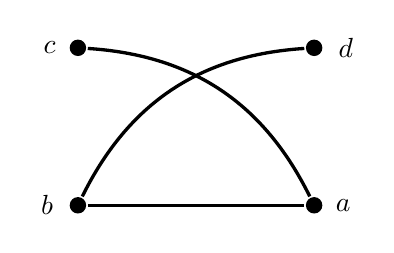
\begin{tikzpicture}[every node/.style={circle, fill=black, inner sep=2.1pt, scale=1}, every path/.style={line width=1.2pt}]
			\node[label=left:$c$] (c) at (0,2) {};
			\node[label=right:$d$] (d) at (3,2) {};
			\node[label=left:$b$] (b) at (0,0) {};
			\node[label=right:$a$] (a) at (3,0) {};
			\draw (b)--(a);
			\draw[bend left=30] (b) to (d);
			\draw[bend left=30] (c) to (a);
		\end{tikzpicture}
		\hspace{2cm}
		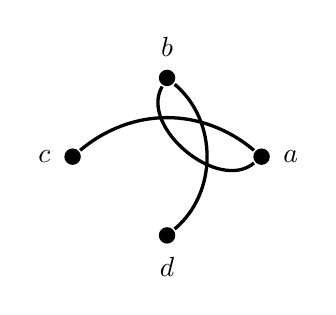
\begin{tikzpicture}[every node/.style={circle, fill=black, inner sep=2.1pt, scale=1}, every path/.style={line width=1.2pt}]
			\node[label=above:$b$] (b) at (0,2) {};
			\node[label=left:$c$] (c) at (-1.2,1) {};
			\node[label=right:$a$] (a) at (1.2,1) {};
			\node[label=below:$d$] (d) at (0,0) {};
			\draw (b) to[out=-120, in=220] (a);
			\draw (c) to[out=40, in=140] (a);
			\draw (b) to[out=-40, in=40] (d);
		\end{tikzpicture}
		\hspace{2cm}
		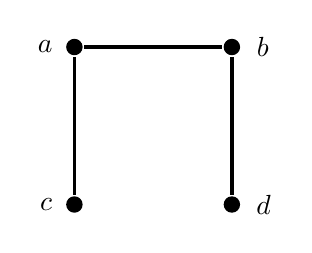
\begin{tikzpicture}[every node/.style={circle, fill=black, inner sep=2.1pt, scale=1}, every path/.style={line width=1.2pt}]
			\node[label=left:$a$] (a) at (0,2) {};
			\node[label=right:$b$] (b) at (2,2) {};
			\node[label=left:$c$] (c) at (0,0) {};
			\node[label=right:$d$] (d) at (2,0) {};
			\draw (a)--(b);
			\draw (a)--(c);
			\draw (b)--(d);
		\end{tikzpicture}
	\end{figure}
\end{example}

ممکن است بین دو رأس از یک گراف، بیش از یک یال وجود داشته باشد. همچنین یک یال ممکن است یک رأس را به خود آن رأس وصل نماید که در این صورت به این یال طوقه (حلقه) گفته می‌شود. گرافی را که در آن هیچ یک از این دو مورد اتفاق نیفتاده باشد، گراف ساده می‌گوییم. ما در این فصل، فقط گراف‌های ساده را بررسی می‌کنیم و منظورمان از گراف، گراف ساده است.

\begin{example}
	گراف‌های زیر، گراف ساده نیستند، بلکه مالتی‌گراف هستند.
	\begin{figure}[H]
		\centering
		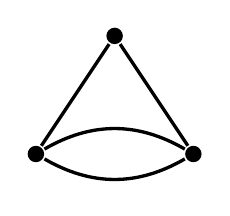
\begin{tikzpicture}[every node/.style={circle, fill=black, inner sep=2.1pt, scale=1}, every path/.style={line width=1.2pt}]
			\node (a) at (1,1.5) {};
			\node (b) at (0,0) {};
			\node (c) at (2,0) {};
			\draw (b) to[out=30, in=150] (c);
			\draw (b) to[out=-30, in=-150] (c);
			\draw (a)--(b);
			\draw (a)--(c);
		\end{tikzpicture}
		\hspace{2cm}
		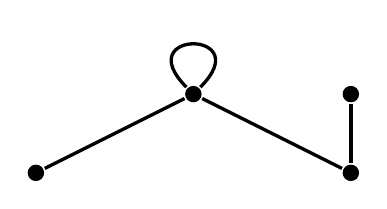
\begin{tikzpicture}[every node/.style={circle, fill=black, inner sep=2.1pt, scale=1}, every path/.style={line width=1.2pt}]
			\node (a) at (0,0) {};
			\node (b) at (2,1) {};
			\node (c) at (4,0) {};
			\node (d) at (4,1) {};
			\draw (a)--(b);
			\draw (b)--(c);
			\draw (c)--(d);
			\draw[loop, looseness=15] (b) to (b);
		\end{tikzpicture}
	\end{figure}
\end{example}

می‌دانیم که اگر مجموعه‌ای $p$ عضو داشته باشد
($p \in \mathbb{Z}^+$)،
تعداد زیرمجموعه‌های دو عضوی آن
$\frac{p(p-1)}{2}$
است. بنابراین اگر گرافی $p$ رأس و $q$ یال داشته باشد، داریم:
$$0 \leq q \leq \frac{p(p-1)}{2}$$

\textbf{مرتبه و اندازه‌ی یک گراف:}
در هر گراف
$G(V,E)$
تعداد اعضای مجموعه‌ی $V$ یعنی $|V(G)|$ را مرتبه‌ی $G$ می‌گوییم و با $p(G)$ یا $p$ نمایش می‌دهیم و تعداد اعضای مجموعه‌ی $E$ یعنی $|E(G)|$ را اندازه‌ی $G$ می‌نامیم و با $q(G)$ یا $q$ نمایش می‌دهیم.

\textbf{درجه‌ی یک رأس:}
درجه‌ی رأس $v$ از گراف $G$ برابر با تعداد یال‌هایی از $G$ است که از رأس $v$ می‌گذرند. این عدد را با
$\deg_G(v)$
و گاهی به‌طور ساده با
$\deg(v)$
نمایش می‌دهیم. اگر
$\deg(v)$
عددی فرد باشد، $v$ را یک رأس فرد و اگر عددی زوج باشد $v$ را یک رأس زوج از گراف $G$ می‌نامیم.

\begin{theorem}
	اگر
	$V=\{v_1,v_2,\cdots,v_p\}$
	مجموعه‌ی رأس‌های گراف $G$ با اندازه‌ی $q$ باشد، آنگاه:
	$$\sum_{i=1}^{p}\deg(v_i) = 2q$$
	\textbf{برهان:}
	هر یال تنها دو سر دارد، یعنی دقیقاً از دو رأس $G$ می‌گذرد و لذا در طرف چپ فرمول بالا هر یال دو بار به حساب می‌آید.
	\qed
	\\ \df \\
	\textbf{نتیجه:}
	تعداد رأس‌های فرد هر گراف، زوج است. \\
	\textbf{برهان:}
\end{theorem}

\textbf{گراف $k$-منتظم:}
گرافی را که درجه‌ی تمام رأس‌های آن با هم مساوی و برابر با عدد $k$ باشند، گراف $k$-منتظم می‌نامیم.

\textbf{رأس تنها و گراف تهی:}
به رأسی که درجه‌ی آن صفر باشد؛ یعنی هیچ یالی به آن متصل نباشد، رأس تنها (ایزوله) می‌گوییم. گرافی را که تمام رأس‌های آن تنها باشند، گراف تهی می‌نامیم.

\textbf{مجموعه‌ی همسایه‌های یک رأس:}
فرض کنیم
$v \in V(G)$.
به مجموعه‌ی رأس‌هایی از گراف $G$ که به رأس $v$ متصل هستند، «همسایگی باز رأس $v$» می‌گوییم و با
$N_G(v)$
نمایش می‌دهیم. اضافه کردن خود رأس $v$ به
$N_G(v)$
«همسایگی بسته‌ی رأس $v$» را به دست می‌دهد که آن را با
$N_G[v]$
نمایش می‌دهیم.
$$N_G(v)=\{u \in V(G) : uv \in E(G)\}$$
$$N_G[v]=N_G(v) \cup \{v\}$$

\textbf{دو یال مجاور:}
دو یال را مجاور گوییم هرگاه رأسی وجود داشته باشد که هر دوی آن‌ها به آن متصل باشند.

\textbf{بزرگ‌ترین و کوچک‌ترین درجه‌ی یک گراف:}
بزرگ‌ترین عدد در بین درجه‌های رأس‌های گراف $G$ را با
$\Delta(G)$
و کوچک‌ترین آن‌ها را با
$\delta(G)$
نمایش می‌دهیم و به ترتیب آن‌ها را مکسیمم و مینیمم درجه‌ی گراف می‌نامیم.

\textbf{زیرگراف:}
یک زیرگراف از $G$ گرافی است که مجموعه‌ی رأس‌های آن زیرمجموعه‌ای از مجموعه‌ی رأس‌های $G$، و مجموعه‌ی یال‌های آن زیرمجموعه‌ای از مجموعه‌ی یال‌های $G$ باشد.

\textbf{مکمل یک گراف:}
مکمل گرافی مانند $G$ که آن را با
$G^c$
نمایش می‌دهیم گرافی است که مجموعه‌ی رأس‌های آن همان مجموعه‌ی رأس‌های $G$ است و بین دو رأس از
$G^c$
یک یال است اگر و تنها اگر بین همان دو رأس در $G$ یالی وجود نداشته باشد.

\textbf{مسیر:}
اگر $u$ و $v$ دو رأس متفاوت از گراف دلخواه $G$ باشند، یک مسیر از $u$ به $v$ از گراف $G$ دنباله‌ای متشکل از
$m+1$
رأس دوبه‌دو متفاوت $G$ است
($m \in \mathbb{Z}^+$)
که از $u$ آغاز و به $v$ ختم می‌شود و هر دو رأس متوالی این دنباله در $G$ مجاورند. عدد $m$ را طول این مسیر از گراف $G$ می‌نامیم. می‌پذیریم که دنباله‌ی متشکل از تنها یک رأس $v$ یک مسیر با طول صفر از $v$ به $v$ از گراف $G$ باشد. اگر یک مسیر از تمام یال‌های $G$ استفاده کند، آنگاه آن را یک مسیر اویلری می‌نامیم. اگر یک مسیر هیچ رأسی را دو بار لمس نکند، آنگاه آن را یک گذر می‌نامیم.

\textbf{دور:}
یک دور از گراف $G$ دنباله‌ای چون
$v_1, v_2, \cdots, v_m, v_{m+1}=v_1$
با شرط
$m \geq 3$
متشکل از
$m+1$
رأس $G$ است که در آن
$v_i$ها،
$1 \leq i \leq m$،
دوبه‌دو متمایزند و هر دو رأس متوالی این دنباله در $G$ مجاورند. عدد $m$ را طول این دور از گراف $G$ می‌نامیم. به دور، مسیر بسته نیز می‌گوییم. گرافی را که تنها از یک دور $n$ رأسی تشکیل شده باشد، با
$C_n$
نمایش می‌دهیم.

\textbf{گراف همبند:}
گراف $G$ را همبند می‌نامیم هرگاه بین هر دو رأس آن مسیری (دقیق‌تر یک گذر) وجود داشته باشد. در غیر این صورت $G$ را ناهمبند می‌نامیم.

\textbf{گراف همیلتونی:}
اگر گراف $G$ از مرتبه‌ی $p$،
$p \geq 3$،
دوری از مرتبه‌ی $p$ داشته باشد (شامل تمام رأس‌های گراف $G$ باشد)، آنگاه $G$ را گراف همیلتونی می‌نامیم. مسیری که شامل تمام رأس‌های یک گراف باشد، مسیر همیلتونی نامیده می‌شود.

\section{احاطه‌گری}
زیرمجموعه‌ی $D$ از مجموعه‌ی رأس‌های گراف $G$ را مجموعه‌ی احاطه‌گر می‌نامیم هرگاه هر رأس از گراف یا در $D$ باشد یا حداقل با یکی از رأس‌های $D$ مجاور باشد.

\section{درخت}
گراف همبندی را که هیچ دور نداشته باشد، درخت می‌گوییم.
\begin{theorem}
	بین هر دو رأس هر درخت مفروض دقیقاً یک مسیر وجود دارد. \\
	\textbf{برهان:}
\end{theorem}

\begin{theorem}
	هر درختی که بیش از یک رأس داشته باشد دست‌کم دو رأس از درجه‌ی یک دارد. \\
	\textbf{برهان:}
\end{theorem}

\begin{theorem}
	اگر $G$ درختی با $p$ رأس و $q$ یال باشد، آنگاه
	$p=q+1$. \\
	\textbf{برهان:}
\end{theorem}

\section{ماتریس و گراف}
\textbf{ماتریس مجاورت گراف:}
به هر گراف $G$ همواره می‌توان ماتریسی چون $A$ با ویژگی‌های زیر نسبت داد. این ماتریس را ماتریس مجاورت گراف $G$ می‌نامیم و آن را با
$A(G)$
یا به‌طور ساده با $A$ نمایش می‌دهیم. همچنین به هر ماتریس با ویژگی‌های زیر می‌توان یک گراف نسبت داد.
\begin{enumerate}
	\item 
	درایه‌های روی قطر اصلی همگی صفرند، زیرا گراف‌های (ساده‌ی) موضوع بحث ما «طوقه» ندارند، یعنی هیچ رأسی با خودش مجاور نیست.
	\item 
	ماتریس $A$ مربعی است.
	\item 
	هر درایه‌ی ماتریس $A$ یا صفر است یا یک، یعنی همواره
	$a_{ij} \in \{0,1\}$.
	\item 
	ماتریس $A$ متقارن است، زیرا اگر
	$v_iv_j \in E$
	آنگاه
	$v_jv_i \in E$.
\end{enumerate}

\begin{theorem}
	فرض کنید $A$ ماتریس مجاورت گراف $G$ با
	$V(G)=\{v_1,\cdots,v_p\}$
	باشد. آنگاه درایه‌ی واقع در سطر $i$ و ستون $i$ ماتریس
	$A^2$
	برابر است با درجه‌ی رأس
	$v_i$
	در گراف $G$. \\ 
	\textbf{برهان:}
\end{theorem}

	\chapter{نظریه‌ی اعداد}
\thispagestyle{empty}

\begin{quote}
	{\lotus
		ریاضیات ملکه‌ی علوم است و نظریه‌ی اعداد ملکه‌ی ریاضیات. \quad - گاوس%
		\LTRfootnote{ Johann Carl Friedrich Gauss}
	}
\end{quote}

	
	\part{احتمال و آمار}
	\chapter{احتمال}
\thispagestyle{empty}

\begin{quote}
	{\lotus
		احتمالات را باید مشابه اندازه‌گیری کمیات فیزیکی تلقی کرد؛ یعنی باید بگوییم که هرگز نمی‌توان آن‌ها را با دقت شناخت بلکه در حد تقریبی مشخص می‌توان شناسایی کرد. \quad - بورل%
		\LTRfootnote{ Felix Edouard Justin Emile Borel}
	}
\end{quote}

	\include{./TeX_files/statistics}
	
	\part{حسابان}
	\chapter{حد و پیوستگی}
\thispagestyle{empty}

\begin{quote}
	{\lotus
		آنالیز ریاضی به اندازه‌ی خود طبیعت گسترده است. \quad - فوریه%
		\LTRfootnote{ Jean Baptiste Joseph Fourier}
	}
\end{quote}

	\chapter{مشتق و کاربردها}
\thispagestyle{empty}

\begin{quote}
	{\lotus
		با در نظر گرفتن ریاضیات از ابتدای دنیا تا زمان نیوتن، نیمی که او انجام داده بسیار بهتر است. \quad - لایبنیتس%
		\LTRfootnote{ Gottfried Wilhelm von Leibnitz}
	}
\end{quote}

	\chapter{انتگرال و کاربردها}
\thispagestyle{empty}

\begin{quote}
	{\lotus
		طبیعت به مشکلات انتگرال‌گیری می‌خندد. \quad - لاپلاس%
		\LTRfootnote{ Pierre-Simon Laplace}
	}
\end{quote}

	
	\backmatter
	\appendix
	\renewcommand{\thechapter}{}
	\part{پیوست‌ها}
	\chapter{پاسخ مسئله‌ها}
\thispagestyle{empty}

\begin{quote}
	{\lotus
		اگر مسئله‌ای وجود دارد که نمی‌توانید حل کنید، مسئله‌ی ساده‌تری وجود دارد که می‌توانید حل کنید؛ آن را بیابید. \quad - پولیا%
	}
\end{quote}
%%%%%%%%%%%%%%%%%%%%%%%%%%%%%%%%%%%%%%%%%%%%%%%
\section*{منطق ریاضی}
\textbf{\ref{loprpedar}}.
در نوبت اول هر دو هم‌زمان می‌گویند: «خیر.» چون هر کدام این‌طور فکر می‌کنند که پیشانی دیگری گلی است و حداقل پیشانی یکی از ما گلی است، پس نمی‌توانم بفهمم پیشانی من گلی است یا نه. در نوبت دوم هر دو هم‌زمان می‌گویند: «بله.» چون بعد از پاسخ قبلی، هر کدام این‌طور فکر می‌کنند که اگر پیشانی من گلی نبود، دیگری باید پاسخ مثبت می‌داد، پس پیشانی من گلی است.

\df \\ \textbf{\ref{loprabccolor}}.
فرض کنید تمبر C قرمز باشد. A پاسخ منفی داده، پس تمبر B قرمز نبوده است. اما اگر چنین است، B نباید پاسخ منفی می‌داد چون از روی پاسخ منفی A و رنگ تمبر C متوجه می‌شد که رنگ تمبرش قرمز نیست. پس تمبر C نمی‌تواند قرمز باشد. با استدلال مشابه (چون تعداد تمبرهای قرمز و زرد یکسان است)، می‌توان گفت که تمبر C نمی‌تواند زرد باشد. بنابراین تمبر C سبز است. اما درباره‌ی رنگ تمبرهای A و B نمی‌توان نظر داد، ممکن است هر کدام از سه رنگ باشند.

\df \\ \textbf{\ref{loprmcgregor}}.
خانه‌ی اول: اگر مرد شوالیه بود، هیچ وقت ادعا نمی‌کرد که او و همسرش هر دو سربازند. در نتیجه، او باید سرباز باشد. از آن‌جا که او سرباز است، جمله‌اش نادرست است؛ پس آن‌ها هر دو سرباز نیستند. این یعنی همسرش باید شوالیه باشد. \\
خانه‌ی دوم: اگر مرد سرباز بود، پس این‌که حداقل یکی از آن‌ها سرباز است، درست می‌شد، اما ممکن نیست، چون سرباز نمی‌تواند راست بگوید. پس مرد شوالیه است. این یعنی ادعایش درست است و حداقل یکی از آن دو سرباز است. از آن‌جا که خودش سرباز نیست، باید همسرش سرباز باشد. \\
خانه‌ی سوم: فرض کنید مرد شوالیه باشد. پس آنچه گفته درست است، پس همسرش باید شوالیه باشد. اگر مرد شوالیه باشد، همسرش هم شوالیه است. این جمله درست است. پس مرد شوالیه است و بنابراین همسرش نیز شوالیه است. \\
خانه‌ی چهارم: نمی‌توان مشخص کرد که مرد شوالیه است یا سرباز، اما نوع همسرش را می‌توان به این صورت مشخص کرد: اگر زن سرباز بود، شوهرش هیچ وقت ادعا نمی‌کرد که نوع او با همسرش یکسان است، چون اگر مرد سرباز باشد، جمله‌ی درست نمی‌گوید. پس زن باید شوالیه باشد.

\df \\ \textbf{\ref{loprladytiger}}.
دو حالت وجود دارد: \\
حالت یکم: علامت در ۱ درست و علامت در ۲ نادرست است. درستی علامت در ۱ نشان می‌دهد که در اتاق ۱ یک دختر و در اتاق ۲ یک ببر است. نادرستی علامت در ۲ نشان می‌دهد که در هر دو اتاق دختر یا در هر دو اتاق ببر است. اما دو نتیجه با هم تناقض دارند، پس حالت یکم ممکن نیست. \\
حالت دوم:  علامت در ۱ نادرست و علامت در ۲ درست است. نادرستی علامت در ۱ نشان می‌دهد که در اتاق ۱ یک ببر و در اتاق ۲ یک دختر است. درستی علامت ۲ نشان می‌دهد که در یکی از دو اتاق دختر و دیگری ببر است که با نتیجه‌ی نادرستی علامت در ۱ منطبق است. پس حالت دوم ممکن است. بنابراین، زندانی باید در ۲ را باز کند.

\df \\ \textbf{\ref{loprpirates}}.
فرض کنید نوشته‌ی صندوقچه‌ی ۲ درست باشد، یعنی صندوقچه‌ی ۲ خالی است. نوشته‌ی صندوقچه‌ی ۱ نادرست است، یعنی صندوقچه‌ی ۱ خالی نیست. نوشته‌ی صندوقچه‌ی ۳ نادرست است، یعنی گنج در صندوقچه‌ی ۲ نیست. بنابراین، گنج در صندوقچه‌ی ۱ است.

\df \\ \textbf{\ref{loprkraig}}.
فرض می‌کنیم دو عبارت X و Y داشته باشیم که یا هر دو درست یا هر دو نادرست باشند. در این صورت اگر یکی از افراد تیمارستان یکی از این عبارت‌ها را باور داشته باشد، عبارت دیگر را نیز باور خواهد داشت. اگر هر دو عبارت درست باشد، در آن صورت هر کدام از افراد تیمارستان که یکی 	از آن‌ها را باور داشته باشد، بایستی عاقل باشد و بنابراین باید عبارت دیگر را باور داشته باشد. اگر هر دو عبارت نادرست باشد، هرکس که یکی از آن‌ها را باور داشته باشد، بایستی دیوانه باشد و باید عبارت دیگر را باور داشته باشد.

دو کمیته‌ی دلخواه مثلاً کمیته‌ی B و C را در نظر می‌گیریم. مجموعه‌ی افرادی را که بدترین دشمنشان در کمیته‌ی B است، U و مجموعه‌ی افرادی را که بهترین دوستشان در کمیته‌ی C است، V می‌نامیم. بنا به مورد ۴، مجموعه‌های U و V نیز هر دو کمیته هستند. بنا به مورد ۵، فردی وجود دارد مثلاً به نام دان که بهترین دوست او مثلاً به نام ادوارد عقیده دارد که او در کمیته‌ی U است و بدترین دشمن او مثلاً به نام فرد عقیده دارد که او در کمیته‌ی V است. اکنون طبق تعریف U اگر بگوییم دان در کمیته‌ی U است، مثل آن است که بگوییم بدترین دشمن او یعنی فرد در کمیته‌ی B است. به بیان دیگر، دو عبارت «دان در U است» و «فرد در کمیته‌ی B است» یا هر دو درست یا هر دو نادرست هستند. چون ادوارد یکی از این دو عبارت یعنی بودن دان در U را باور دارد، پس بایستی عبارت دیگر یعنی بودن فرد در کمیته‌ی B را نیز باور داشته باشد. پس ادوارد عقیده دارد که فرد در کمیته‌ی B است.

از سوی دیگر، فرد عقیده دارد که دان در کمیته‌ی V است. طبق تعریف \lr{V}، دان فقط در صورتی عضو V خواهد بود که دوست او ادوارد عضو کمیته‌ی C باشد، یعنی این دو عبارت یا هر دو درست یا هر دو نادرست هستند. اما چون فرد عقیده دارد که دان عضو V است، فرد بایستی عقیده داشته باشد که ادوارد عضو کمیته‌ی C است.

اکنون کمیته‌ی بیماران و کمیته‌ی پزشکان را مطابق موردهای ۱ و ۲ در نظر بگیرید و این دو کمیته را به ترتیب به‌جای کمیته‌های B و C فرض کنید. ‌دو نفر مانند ادوارد و فرد وجود دارند که دارای عقیده‌های زیر هستند: ادوارد عقیده دارد که فرد در کمیته‌ی بیماران است و فرد عقیده دارد که ادوارد در کمیته‌ی پزشکان است.

فرد یا عاقل است یا دیوانه. فرض کنیم عاقل باشد. در این صورت، باور او درست است، یعنی ادوارد واقعاً پزشک است. اگر ادوارد دیوانه باشد، در این صورت پزشکی دیوانه است. اگر ادوارد عاقل باشد، در این صورت باور او درست است، یعنی فرد بیمار و بنا به فرض، بیماری عاقل است. به این ترتیب ثابت می‌شود که اگر فرد عاقل باشد، یا او بیماری عاقل یا ادوارد پزشکی دیوانه است.

اکنون فرض کنیم که فرد دیوانه باشد. در این صورت، باور او نادرست است، یعنی ادوارد بیمار است. اگر ادوارد بیمار باشد، در این صورت بیماری عاقل است. اگر ادوارد دیوانه باشد، در این صورت باور او نادرست است و نتیجه می‌شود که فرد پزشک و بنا به فرض، پزشکی دیوانه است. به این ترتیب ثابت می‌شود که اگر فرد دیوانه باشد، یا او پزشکی دیوانه است یا ادوارد بیماری عاقل است.

بنابراین، یکی از این دو نفر، یعنی ادوارد یا فرد، بایستی یا پزشکی دیوانه یا بیماری عاقل باشد.

\df \\ \textbf{\ref{lopr4cab45}}.
حداقل باید دو کارت $B$ و ۴ را برگردانیم. کارت ۵ تأثیری ندارد چون عددی فرد است. کارت $A$ نیز تأثیری ندارد چون حرف صدادار است.

\df \\ \textbf{\ref{loprrttp}}.
\begin{table}[H]
	\begin{latin}
		\centering
		\begin{tabular}{c|c|c|c}
			$p$ & $q$ & $p \vee q$ & $(p \vee q) \rightarrow q$ \\
			\hline
			T & T & T & T \\
			T & F & T & F \\
			F & T & T & T \\
			F & F & F & T 
		\end{tabular}
		\qquad \qquad
		\begin{tabular}{c|c|c|c|c}
			$p$ & $q$ & $\neg p$ & $p \leftrightarrow q$ & $\neg p \wedge (p \leftrightarrow q)$ \\
			\hline
			T & T & F & T & F \\
			T & F & F & F & F \\
			F & T & T & T & T \\
			F & F & T & T & T
		\end{tabular}
	\end{latin}
\end{table}

\df \\ \textbf{\ref{loprpqreqx}}.
دو روش برای نوشتن گزاره‌ی معادل وجود دارد. در روش اول سطرهایی را که ارزش گزاره‌ی $X$ درست است در نظر می‌گیریم. در روش دوم سطرهایی را که ارزش گزاره‌ی $X$ نادرست است در نظر می‌گیریم. \\
گزاره‌ی اول:
$$(p \wedge \neg q \wedge r) \vee (\neg p \wedge q \wedge \neg r) \vee (\neg p \wedge \neg q \wedge q)$$
گزاره‌ی دوم:
$$(\neg p \vee \neg q \vee \neg r) \wedge (\neg p \vee \neg q \vee r) \wedge (\neg p \vee q \vee r) \wedge (p \vee q \vee r)$$
%%%%%%%%%%%%%%%%%%%%%%%%%%%%%%%%%%%%%%%%%%%%%%
\section*{اعداد}
\textbf{\ref{nupr1000prnu}}.
عددهای
$$1001!+2 \ , \ 1001!+3 \ , \ \cdots \ , \ 1001!+1000 \ , \ 1001!+1001$$
هزار عدد متوالی‌اند که هیچ‌کدام اول نیستند.
%%%%%%%%%%%%%%%%%%%%%%%%%%%%%%%%%%%%%%%%%%%%%%%
\section*{استدلال و برهان}
%%%%%%%%%%%%%%%%%%%%%%%%%%%%%%%%%%%%%%%%%%%%%%%
\section*{نظریه‌ی مجموعه‌ها}
%%%%%%%%%%%%%%%%%%%%%%%%%%%%%%%%%%%%%%%%%%%%%%%
\section*{معادلات و نامعادلات}
\textbf{\ref{arb+bra}}.
با توجه به فرمول مجموع و حاصل‌ضرب جواب‌های معادله‌ی درجه‌ی دوم داریم:
$$\alpha + \beta = \frac{-(-12)}{1} = 12 \ , \quad \alpha \beta = \frac{4}{1} = 4$$
بنابراین:
$$(\alpha \sqrt{\beta} + \beta \sqrt{\alpha})^2 = \alpha^2\beta + \beta^2\alpha + 2\alpha\beta\sqrt{\alpha\beta} = \alpha\beta(\alpha+\beta)+2\alpha\beta\sqrt{\alpha\beta} = 4(12)+2(4)(\sqrt{4}) = 64$$
خواسته‌ی مسئله برابر ریشه‌ی دوم عبارت بالاست، اما باید در نظر بگیریم که ریشه‌ی دوم ۶۴ دو جواب دارد: ۸ و $-8$. با توجه به این‌که مجموع و حاصل‌ضرب ریشه‌های عبارت درجه‌ی دوم، هر دو مثبت هستند، پس هر دو ریشه مثبت است و در نتیجه مقدار $-8$ قابل قبول نیست. پس جواب مسئله برابر با ۸ است.
%%%%%%%%%%%%%%%%%%%%%%%%%%%%%%%%%%%%%%%%%%%%%%%
\section*{ماتریس و دترمینان}

\df \\ \textbf{\ref{maprabprob}}.
داریم:
$A+B=
\begin{bmatrix}
	a & b-7 \\
	-1 & 1
\end{bmatrix}$.
شرط وارون‌پذیری این است که
$|A+B| \neq 0$،
بنابراین:
$$|A+B|=a+b-7 \neq 0 \Rightarrow a+b \neq 7$$
بنابراین حالاتی از
$(a,b)$
که مجموع دو تاس برابر ۷ است، قابل قبول نیست، یعنی:
$$\text{حالات نامطلوب}={(1,6),(2,5),(3,4),(4,3),(5,2),(6,1)}$$
$$\Rightarrow n(\text{مطلوب}) =36-6=30 \Rightarrow P(\text{مطلوب})=\frac{30}{36}=\frac{5}{6}$$

\df \\ \textbf{\ref{maprr3adet}}.
از دو طرف تساوی، دترمینان می‌گیریم.
\[
\left| \sqrt{3}A \right| =
\begin{vmatrix}
	-2 & |A|+1 \\
	3|A| & -|A|
\end{vmatrix}
\Rightarrow
\left( \sqrt{3} \right)^2 |A| = 2|A| - 3|A|^2 -3|A|
\Rightarrow
3|A|^2+4|A|=0
\Rightarrow
\begin{cases}
	|A|=0 \\
	|A|=-\frac{4}{3}
\end{cases}
\]
از آن‌جا که $A$ وارون‌پذیر است،
$|A| \neq 0$.
پس تنها جواب قابل قبول
$|A| = -\frac{4}{3}$
است.

\df
%%%%%%%%%%%%%%%%%%%%%%%%%%%%%%%%%%%%%%%%%%%%%%%

	\chapter{واژه‌نامه‌ی فارسی - انگلیسی}
%%%%%%%%%%%%%%%%%%%%%%%%%%%%%%%
%%%%%%%%%%%%%%%%%%%%%%%%%%%%%%%
ریاضیات
\dotfill
\lr{Mathematics}
\\
%%%%%%%%%%%%%%%%%%%%%%%%%%%%%%%
%%%%%%%%%%%%%%%%%%%%%%%%%%%%%%%
\section*{مبانی}
%%%%%%%%%%%%%%%%%%%%%%%%%%%%%%%
منطق
\dotfill
\lr{Logic}
\\
%%%%%%%%%%%%%%%%%%%%%%%%%%%%%%%
گزاره
\dotfill
\lr{Proposition}
\\
%%%%%%%%%%%%%%%%%%%%%%%%%%%%%%%
درست
\dotfill
\lr{True}
\\
%%%%%%%%%%%%%%%%%%%%%%%%%%%%%%%
نادرست / غلط
\dotfill
\lr{False}
\\
%%%%%%%%%%%%%%%%%%%%%%%%%%%%%%%
اثبات برگشت‌پذیر
\dotfill
\lr{Proof by Equivalence}
\\
%%%%%%%%%%%%%%%%%%%%%%%%%%%%%%%
استدلال
\dotfill
\lr{Reasoning}
\\
%%%%%%%%%%%%%%%%%%%%%%%%%%%%%%%
استقرا
\dotfill
\lr{Induction}
\\
%%%%%%%%%%%%%%%%%%%%%%%%%%%%%%%
استنتاج
\dotfill
\lr{Inference}
\\
%%%%%%%%%%%%%%%%%%%%%%%%%%%%%%%
برهان
\dotfill
\lr{Proof}
\\
%%%%%%%%%%%%%%%%%%%%%%%%%%%%%%%
برهان خلف
\dotfill
\lr{Proof by Contradiction / Reductio ad absurdum}
\\
%%%%%%%%%%%%%%%%%%%%%%%%%%%%%%%
حدس
\dotfill
\lr{Conjecture}
\\
%%%%%%%%%%%%%%%%%%%%%%%%%%%%%%%
حکم / ادعا
\dotfill
\lr{Assertion / Claim}
\\
%%%%%%%%%%%%%%%%%%%%%%%%%%%%%%%
عکس نقیض
\dotfill
\lr{Contrapositive}
\\
%%%%%%%%%%%%%%%%%%%%%%%%%%%%%%%
فرض
\dotfill
\lr{Assumption}
\\
%%%%%%%%%%%%%%%%%%%%%%%%%%%%%%%
قضیه
\dotfill
\lr{Theorem}
\\
%%%%%%%%%%%%%%%%%%%%%%%%%%%%%%%
مثال نقض
\dotfill
\lr{Counterexample}
\\
%%%%%%%%%%%%%%%%%%%%%%%%%%%%%%%
نتیجه
\dotfill
\lr{Corollary}
\\
%%%%%%%%%%%%%%%%%%%%%%%%%%%%%%%
مجموعه
\dotfill
\lr{Set}
\\
%%%%%%%%%%%%%%%%%%%%%%%%%%%%%%%
اثبات مستقیم
\dotfill
\lr{Direct Proof}
\\
%%%%%%%%%%%%%%%%%%%%%%%%%%%%%%%
%%%%%%%%%%%%%%%%%%%%%%%%%%%%%%%
\section*{جبر}
%%%%%%%%%%%%%%%%%%%%%%%%%%%%%%%
کلمه
\dotfill
\lr{word}
\\
%%%%%%%%%%%%%%%%%%%%%%%%%%%%%%%
%%%%%%%%%%%%%%%%%%%%%%%%%%%%%%%
\section*{مثلثات}
%%%%%%%%%%%%%%%%%%%%%%%%%%%%%%%
کلمه
\dotfill
\lr{word}
\\
%%%%%%%%%%%%%%%%%%%%%%%%%%%%%%%
%%%%%%%%%%%%%%%%%%%%%%%%%%%%%%%
\section*{هندسه}
%%%%%%%%%%%%%%%%%%%%%%%%%%%%%%%
کلمه
\dotfill
\lr{word}
\\
%%%%%%%%%%%%%%%%%%%%%%%%%%%%%%%
%%%%%%%%%%%%%%%%%%%%%%%%%%%%%%%
\section*{جبر خطی}
%%%%%%%%%%%%%%%%%%%%%%%%%%%%%%%
ترانهاده
\dotfill
\lr{Transpose}
\\
%%%%%%%%%%%%%%%%%%%%%%%%%%%%%%%
دترمینان
\dotfill
\lr{Determinant}
\\
%%%%%%%%%%%%%%%%%%%%%%%%%%%%%%%
درایه
\dotfill
\lr{Entry/Element}
\\
%%%%%%%%%%%%%%%%%%%%%%%%%%%%%%%
دستگاه معادلات خطی
\dotfill
\lr{System of Linear Equations}
\\
%%%%%%%%%%%%%%%%%%%%%%%%%%%%%%%
دستور ساروس
\dotfill
\lr{Sarrus's Rule}
\\
%%%%%%%%%%%%%%%%%%%%%%%%%%%%%%%
دستور کرامر
\dotfill
\lr{Cramer's Rule}
\\
%%%%%%%%%%%%%%%%%%%%%%%%%%%%%%%
ستون
\dotfill
\lr{Column}
\\
%%%%%%%%%%%%%%%%%%%%%%%%%%%%%%%
سطر
\dotfill
\lr{Row}
\\
%%%%%%%%%%%%%%%%%%%%%%%%%%%%%%%
ماتریس
\dotfill
\lr{Matrix}
\\
%%%%%%%%%%%%%%%%%%%%%%%%%%%%%%%
ماتریس بالامثلثی
\dotfill
\lr{Upper Triangular Matrix}
\\
%%%%%%%%%%%%%%%%%%%%%%%%%%%%%%%
ماتریس پادمتقارن
\dotfill
\lr{Skew-Symmetric Matrix}
\\
%%%%%%%%%%%%%%%%%%%%%%%%%%%%%%%
ماتریس پایین‌مثلثی
\dotfill
\lr{Lower Triangular Matrix}
\\
%%%%%%%%%%%%%%%%%%%%%%%%%%%%%%%
ماتریس صفر
\dotfill
\lr{Zero/Null Matrix}
\\
%%%%%%%%%%%%%%%%%%%%%%%%%%%%%%%
ماتریس ضرایب
\dotfill
\lr{Coefficient Matrix}
\\
%%%%%%%%%%%%%%%%%%%%%%%%%%%%%%%
ماتریس قطری
\dotfill
\lr{Diagonal Matrix}
\\
%%%%%%%%%%%%%%%%%%%%%%%%%%%%%%%
ماتریس متقارن
\dotfill
\lr{Symmetric Matrix}
\\
%%%%%%%%%%%%%%%%%%%%%%%%%%%%%%%
ماتریس مربعی
\dotfill
\lr{Square Matrix}
\\
%%%%%%%%%%%%%%%%%%%%%%%%%%%%%%%
ماتریس وارون
\dotfill
\lr{Inverse Matrix}
\\
%%%%%%%%%%%%%%%%%%%%%%%%%%%%%%%
ماتریس همانی
\dotfill
\lr{Identity Matrix}
\\
%%%%%%%%%%%%%%%%%%%%%%%%%%%%%%%
کهاد
\dotfill
\lr{Minor}
\\
%%%%%%%%%%%%%%%%%%%%%%%%%%%%%%%
همسازه
\dotfill
\lr{Cofactor}
\\
%%%%%%%%%%%%%%%%%%%%%%%%%%%%%%%
%%%%%%%%%%%%%%%%%%%%%%%%%%%%%%%
\section*{ریاضیات گسسته}
%%%%%%%%%%%%%%%%%%%%%%%%%%%%%%%
کلمه
\dotfill
\lr{word}
\\
%%%%%%%%%%%%%%%%%%%%%%%%%%%%%%%
%%%%%%%%%%%%%%%%%%%%%%%%%%%%%%%
\section*{احتمال و آمار}
%%%%%%%%%%%%%%%%%%%%%%%%%%%%%%%
کلمه
\dotfill
\lr{word}
\\
%%%%%%%%%%%%%%%%%%%%%%%%%%%%%%%
%%%%%%%%%%%%%%%%%%%%%%%%%%%%%%%
\section*{حسابان}
%%%%%%%%%%%%%%%%%%%%%%%%%%%%%%%
کلمه
\dotfill
\lr{word}
\\
%%%%%%%%%%%%%%%%%%%%%%%%%%%%%%%

	\cleardoublepage
\addcontentsline{toc}{chapter}{مراجع}

\renewcommand{\bibname}{مراجع}
\begin{thebibliography}{99}
	\begin{LTRbibitems}
		\resetlatinfont
		\bibitem{EngRef1}
		Pure Mathematics 1, Sue Pemberton, Julianne Hughes, Cambridge University Press, 2018.
		\bibitem{EngRef2}
		Pure Mathematics 2 \& 3, Sue Pemberton, Cambridge University Press, 2018.
		\bibitem{EngRef3}
		Mathematics: Analysis and Approaches, Higher Level, Jennifer Chang Wathall, and others, Oxford University Press, 2019.
		\bibitem{EngRef4}
		Mathematics: Applications and Interpretation, Higher Level, Suzanne Doering, and others, Oxford University Press, 2019.
		\bibitem{EngRef5}
		Functions 11, Marian Small, Chris Kirkpatrick, and others, Nelson, 2008.
		\bibitem{EngRef6}
		Functions 12, Marian Small, Chris Kirkpatrick, and others, Nelson, ?.
		\bibitem{EngRef7}
		Forever Undecided, Raymond Smullyan, Alfred A. Knopf, Inc., 1987.
		\bibitem{EngRef8}
		Mathematics: Core Topics HL, Micheal Haese, and others, Haese \& Harris, 2019.
		\bibitem{EngRef9}
		Discrete Mathematics and Its Applications, Kenneth H. Rosen, Eighth Edition, McGraw-Hill, 2019.
	\end{LTRbibitems}
	\bibitem{PerRef1}
	جبر، سال چهارم ریاضی، وزارت آموزش و پرورش، ۱۳۵۲.
	\bibitem{PerRef2}
	جبر، سال پنجم ریاضی، وزارت آموزش و پرورش، ۱۳۵۴.
	\bibitem{PerRef3}
	جبر، سال ششم ریاضی، وزارت آموزش و پرورش، ۱۳۴۸.
	\bibitem{PerRef4}
	جبر، سال اول آموزش متوسطه‌ی عمومی علوم تجربی و ریاضی، وزارت آموزش و پرورش، ۱۳۷۰.
	\bibitem{PerRef5}
	حساب و جبر، سال دوم آموزش متوسطه‌ی عمومی ریاضی و فیزیک، وزارت آموزش و پرورش، ۱۳۷۱.
	\bibitem{PerRef6}
	جبر، سال سوم آموزش متوسطه‌ی عمومی ریاضی و فیزیک، وزارت آموزش و پرورش، ۱۳۷۳.
	\bibitem{PerRef7}
	جبر و آنالیز، سال چهارم آموزش متوسطه‌ی عمومی ریاضی و فیزیک، وزارت آموزش و پرورش، ؟.
	\bibitem{PerRef8}
	مثلثات، سال ششم ریاضی، وزارت آموزش و پرورش، ۱۳۵۴.
	\bibitem{PerRef9}
	مثلثات، سال دوم آموزش متوسطه‌ی عمومی ریاضی و فیزیک، وزارت آموزش و پرورش، ۱۳۷۲.
	\bibitem{PerRef10}
	مثلثات، سال سوم آموزش متوسطه‌ی عمومی ریاضی و فیزیک، وزارت آموزش و پرورش، ۱۳۶۰.
	\bibitem{PerRef11}
	حساب استدلالی، سال ششم ریاضی، وزارت آموزش و پرورش، ۱۳۵۵.
	\bibitem{PerRef12}
	ریاضیات ۱، حسین انصاری، سیامک قادر، ویرایش چهارم، مبتکران، ۱۳۹۰.
	\bibitem{PerRef13}
	ریاضیات ۲، حسین انصاری، سیامک قادر، مبتکران، ۱۳۸۹.
	\bibitem{PerRef14}
	ریاضیات محاسبه‌ای، جلد اول، پرویز شهریاری، فردوس، چاپ چهارم: ۱۳۷۷.
	\bibitem{PerRef15}
	ریاضیات محاسبه‌ای، جلد دوم، پرویز شهریاری، مجید، چاپ سوم: ۱۳۷۷.
	\bibitem{PerRef16}
	ریاضیات محاسبه‌ای، جلد سوم، پرویز شهریاری، مجید، چاپ سوم: ۱۳۷۷.
	\bibitem{PerRef17}
	ریاضیات محاسبه‌ای، جلد چهارم، پرویز شهریاری، فردوس، ۱۳۷۵.
	\bibitem{PerRef18}
	ریاضیات محاسبه‌ای، جلد پنجم، پرویز شهریاری، فردوس، ۱۳۷۶.
	\bibitem{PerRef19}
	در حل مسأله‌های ریاضی اشتباه نکنیم، پرویز شهریاری، تهران، ۱۳۷۵.
	\bibitem{PerRef20}
	معماهایی در منطق ریاضی (بانو یا ببر؟)، ریموند اسمولیان، ترجمه‌ی محمد شریف‌زاده، فاطمی، ۱۳۶۶.
	\bibitem{PerRef21}
	نقل قول‌های ریاضی، کیمیا نارنجانی، مجید میرزاوزیری، ۱۳۸۷.
	\bibitem{PerRef22}
	هندسه‌ی تحلیلی و جبر خطی، دوره‌ی پیش‌دانشگاهی رشته‌ی علوم ریاضی، وزارت آموزش و پرورش، چاپ هفدهم: ۱۳۹۶.
	\bibitem{PerRef23}
	هندسه (۳)، پایه‌ی دوازدهم دوره‌ی دوم متوسطه، وزارت آموزش و پرورش، چاپ هفتم: ۱۴۰۳.
	\bibitem{PerRef24}
	مبانی ماتریس‌ها و جبر خطی، محمدحسن بیژن‌زاده، و دیگران، دانشگاه پیام نور، ۱۳۸۹.
	\bibitem{PerRef25}
	جبر و احتمال، سال سوم آموزش متوسطه رشته‌ی ریاضی و فیزیک، وزارت آموزش و پرورش، ۱۳۹۵.
	\bibitem{PerRef26}
	مبانی ریاضیات، محسن خانی، ۱۴۰۲.
	\bibitem{PerRef27}
	آزمون‌های آزمایشی ماز.
	\bibitem{PerRef28}
	آزمون‌های آزمایشی مدارس سمپاد مشهد، دپارتمان کنکور شهید هاشمی‌نژاد ۱ مشهد.
	\bibitem{PerRef29}
	نردبان المپیاد ریاضی - جبر (مرحله‌ی اول)، مهدی صفا، گچ، چاپ دوم: ۱۳۹۸.
	\bibitem{PerRef30}
	ریاضیات گسسته، دوره‌ی پیش‌دانشگاهی رشته‌ی علوم ریاضی، وزارت آموزش و پرورش، چاپ بیست و سوم: ۱۳۹۶.
	\bibitem{PerRef31}
	گشتی در ترکیبیات: مقدمه‌ای بر شمارش و نظریه‌ی گراف، میکلوش بونا، ترجمه‌ی مهدی نجفی‌خواه، ۱۴۰۴.
\end{thebibliography}

%\cleardoublepage
%\chapter{منابع تصاویر}
%شکل \ref{fig1.1}
%\dotfill
%\lr{ref}
%\\
%%%%%%%%%%%%%%%%%%%%%%%%%%%%%%%%%%%
%شکل \ref{fig1.2}
%\dotfill
%ref
%\\
%%%%%%%%%%%%%%%%%%%%%%%%%%%%%%%%%%%
%شکل \ref{fig1.3}
%\dotfill
%ref
%\\
%%%%%%%%%%%%%%%%%%%%%%%%%%%%%%%%%%%
%شکل \ref{fig1.4}
%\dotfill
%\href{https://}
%\\
%%%%%%%%%%%%%%%%%%%%%%%%%%%%%%%%%%%

	
%	\begin{titlepage}
%		\newpage\null
%		\newgeometry{margin=0cm}
%		\thispagestyle{empty}
%		\noindent
%		\centering
%		\includegraphics[width=\paperwidth, height=\paperheight]{./Images/back-cover.png}
%	\end{titlepage}
	
\end{document}
